\documentclass[twoside]{book}

% Packages required by doxygen
\usepackage{fixltx2e}
\usepackage{calc}
\usepackage{doxygen}
\usepackage{graphicx}
\usepackage[utf8]{inputenc}
\usepackage{makeidx}
\usepackage{multicol}
\usepackage{multirow}
\PassOptionsToPackage{warn}{textcomp}
\usepackage{textcomp}
\usepackage[nointegrals]{wasysym}
\usepackage[table]{xcolor}

% Font selection
\usepackage[T1]{fontenc}
\usepackage[scaled=.90]{helvet}
\usepackage{courier}
\usepackage{amssymb}
\usepackage{sectsty}
\renewcommand{\familydefault}{\sfdefault}
\allsectionsfont{%
  \fontseries{bc}\selectfont%
  \color{darkgray}%
}
\renewcommand{\DoxyLabelFont}{%
  \fontseries{bc}\selectfont%
  \color{darkgray}%
}
\newcommand{\+}{\discretionary{\mbox{\scriptsize$\hookleftarrow$}}{}{}}

% Page & text layout
\usepackage{geometry}
\geometry{%
  a4paper,%
  top=2.5cm,%
  bottom=2.5cm,%
  left=2.5cm,%
  right=2.5cm%
}
\tolerance=750
\hfuzz=15pt
\hbadness=750
\setlength{\emergencystretch}{15pt}
\setlength{\parindent}{0cm}
\setlength{\parskip}{0.2cm}
\makeatletter
\renewcommand{\paragraph}{%
  \@startsection{paragraph}{4}{0ex}{-1.0ex}{1.0ex}{%
    \normalfont\normalsize\bfseries\SS@parafont%
  }%
}
\renewcommand{\subparagraph}{%
  \@startsection{subparagraph}{5}{0ex}{-1.0ex}{1.0ex}{%
    \normalfont\normalsize\bfseries\SS@subparafont%
  }%
}
\makeatother

% Headers & footers
\usepackage{fancyhdr}
\pagestyle{fancyplain}
\fancyhead[LE]{\fancyplain{}{\bfseries\thepage}}
\fancyhead[CE]{\fancyplain{}{}}
\fancyhead[RE]{\fancyplain{}{\bfseries\leftmark}}
\fancyhead[LO]{\fancyplain{}{\bfseries\rightmark}}
\fancyhead[CO]{\fancyplain{}{}}
\fancyhead[RO]{\fancyplain{}{\bfseries\thepage}}
\fancyfoot[LE]{\fancyplain{}{}}
\fancyfoot[CE]{\fancyplain{}{}}
\fancyfoot[RE]{\fancyplain{}{\bfseries\scriptsize Generated on Thu Nov 20 2014 16\+:42\+:33 for libsensorj by Doxygen }}
\fancyfoot[LO]{\fancyplain{}{\bfseries\scriptsize Generated on Thu Nov 20 2014 16\+:42\+:33 for libsensorj by Doxygen }}
\fancyfoot[CO]{\fancyplain{}{}}
\fancyfoot[RO]{\fancyplain{}{}}
\renewcommand{\footrulewidth}{0.4pt}
\renewcommand{\chaptermark}[1]{%
  \markboth{#1}{}%
}
\renewcommand{\sectionmark}[1]{%
  \markright{\thesection\ #1}%
}

% Indices & bibliography
\usepackage{natbib}
\usepackage[titles]{tocloft}
\setcounter{tocdepth}{3}
\setcounter{secnumdepth}{5}
\makeindex

% Hyperlinks (required, but should be loaded last)
\usepackage{ifpdf}
\ifpdf
  \usepackage[pdftex,pagebackref=true]{hyperref}
\else
  \usepackage[ps2pdf,pagebackref=true]{hyperref}
\fi
\hypersetup{%
  colorlinks=true,%
  linkcolor=blue,%
  citecolor=blue,%
  unicode%
}

% Custom commands
\newcommand{\clearemptydoublepage}{%
  \newpage{\pagestyle{empty}\cleardoublepage}%
}


%===== C O N T E N T S =====

\begin{document}

% Titlepage & ToC
\hypersetup{pageanchor=false,
             bookmarks=true,
             bookmarksnumbered=true,
             pdfencoding=unicode
            }
\pagenumbering{roman}
\begin{titlepage}
\vspace*{7cm}
\begin{center}%
{\Large libsensorj }\\
\vspace*{1cm}
{\large Generated by Doxygen 1.8.8}\\
\vspace*{0.5cm}
{\small Thu Nov 20 2014 16:42:33}\\
\end{center}
\end{titlepage}
\clearemptydoublepage
\tableofcontents
\clearemptydoublepage
\pagenumbering{arabic}
\hypersetup{pageanchor=true}

%--- Begin generated contents ---
\chapter{Namespace Index}
\section{Packages}
Here are the packages with brief descriptions (if available)\+:\begin{DoxyCompactList}
\item\contentsline{section}{\hyperlink{namespacecom}{com} }{\pageref{namespacecom}}{}
\item\contentsline{section}{\hyperlink{namespacecom_1_1libsensorj}{com.\+libsensorj} }{\pageref{namespacecom_1_1libsensorj}}{}
\item\contentsline{section}{\hyperlink{namespacecom_1_1libsensorj_1_1concreteevent}{com.\+libsensorj.\+concreteevent} }{\pageref{namespacecom_1_1libsensorj_1_1concreteevent}}{}
\item\contentsline{section}{\hyperlink{namespacecom_1_1libsensorj_1_1concretefactory}{com.\+libsensorj.\+concretefactory} }{\pageref{namespacecom_1_1libsensorj_1_1concretefactory}}{}
\item\contentsline{section}{\hyperlink{namespacecom_1_1libsensorj_1_1concretesensor}{com.\+libsensorj.\+concretesensor} }{\pageref{namespacecom_1_1libsensorj_1_1concretesensor}}{}
\item\contentsline{section}{\hyperlink{namespacecom_1_1libsensorj_1_1examples}{com.\+libsensorj.\+examples} }{\pageref{namespacecom_1_1libsensorj_1_1examples}}{}
\item\contentsline{section}{\hyperlink{namespacecom_1_1libsensorj_1_1interfaces}{com.\+libsensorj.\+interfaces} }{\pageref{namespacecom_1_1libsensorj_1_1interfaces}}{}
\item\contentsline{section}{\hyperlink{namespacecom_1_1libsensorj_1_1model}{com.\+libsensorj.\+model} }{\pageref{namespacecom_1_1libsensorj_1_1model}}{}
\item\contentsline{section}{\hyperlink{namespacecom_1_1pi4j}{com.\+pi4j} }{\pageref{namespacecom_1_1pi4j}}{}
\item\contentsline{section}{\hyperlink{namespacecom_1_1pi4j_1_1examples}{com.\+pi4j.\+examples} }{\pageref{namespacecom_1_1pi4j_1_1examples}}{}
\end{DoxyCompactList}

\chapter{Hierarchical Index}
\section{Class Hierarchy}
This inheritance list is sorted roughly, but not completely, alphabetically\+:\begin{DoxyCompactList}
\item \contentsline{section}{com.\+pi4j.\+examples.\+Blink\+Gpio\+Example}{\pageref{classcom_1_1pi4j_1_1examples_1_1BlinkGpioExample}}{}
\item \contentsline{section}{com.\+pi4j.\+examples.\+Blink\+Trigger\+Gpio\+Example}{\pageref{classcom_1_1pi4j_1_1examples_1_1BlinkTriggerGpioExample}}{}
\item \contentsline{section}{com.\+pi4j.\+examples.\+Control\+Gpio\+Example}{\pageref{classcom_1_1pi4j_1_1examples_1_1ControlGpioExample}}{}
\item \contentsline{section}{com.\+pi4j.\+examples.\+Cylon\+Gpio\+Example}{\pageref{classcom_1_1pi4j_1_1examples_1_1CylonGpioExample}}{}
\item \contentsline{section}{com.\+libsensorj.\+examples.\+D\+H\+T11\+Temperature\+Example}{\pageref{classcom_1_1libsensorj_1_1examples_1_1DHT11TemperatureExample}}{}
\item \contentsline{section}{com.\+pi4j.\+examples.\+Example}{\pageref{classcom_1_1pi4j_1_1examples_1_1Example}}{}
\item \contentsline{section}{com.\+pi4j.\+examples.\+Frequency\+Gpio\+Example}{\pageref{classcom_1_1pi4j_1_1examples_1_1FrequencyGpioExample}}{}
\item \contentsline{section}{com.\+pi4j.\+examples.\+I2\+C\+Wii\+Motion\+Plus\+Example}{\pageref{classcom_1_1pi4j_1_1examples_1_1I2CWiiMotionPlusExample}}{}
\item \contentsline{section}{com.\+libsensorj.\+interfaces.\+I\+Event}{\pageref{interfacecom_1_1libsensorj_1_1interfaces_1_1IEvent}}{}
\begin{DoxyCompactList}
\item \contentsline{section}{com.\+libsensorj.\+concreteevent.\+Humidity\+Event}{\pageref{classcom_1_1libsensorj_1_1concreteevent_1_1HumidityEvent}}{}
\item \contentsline{section}{com.\+libsensorj.\+concreteevent.\+Temperature\+Event}{\pageref{classcom_1_1libsensorj_1_1concreteevent_1_1TemperatureEvent}}{}
\item \contentsline{section}{com.\+libsensorj.\+concreteevent.\+Ultrasonic\+Range\+Finder\+Event}{\pageref{classcom_1_1libsensorj_1_1concreteevent_1_1UltrasonicRangeFinderEvent}}{}
\end{DoxyCompactList}
\item \contentsline{section}{com.\+libsensorj.\+interfaces.\+I\+Sensor}{\pageref{interfacecom_1_1libsensorj_1_1interfaces_1_1ISensor}}{}
\begin{DoxyCompactList}
\item \contentsline{section}{com.\+libsensorj.\+concretesensor.\+D\+H\+T11\+Humidity}{\pageref{classcom_1_1libsensorj_1_1concretesensor_1_1DHT11Humidity}}{}
\item \contentsline{section}{com.\+libsensorj.\+concretesensor.\+D\+H\+T11\+Temperature}{\pageref{classcom_1_1libsensorj_1_1concretesensor_1_1DHT11Temperature}}{}
\item \contentsline{section}{com.\+libsensorj.\+concretesensor.\+Ultrasonic\+Hcsr04}{\pageref{classcom_1_1libsensorj_1_1concretesensor_1_1UltrasonicHcsr04}}{}
\end{DoxyCompactList}
\item \contentsline{section}{com.\+libsensorj.\+interfaces.\+I\+Sensor\+Factory}{\pageref{interfacecom_1_1libsensorj_1_1interfaces_1_1ISensorFactory}}{}
\begin{DoxyCompactList}
\item \contentsline{section}{com.\+libsensorj.\+concretefactory.\+Humidity\+Sensor\+Factory}{\pageref{classcom_1_1libsensorj_1_1concretefactory_1_1HumiditySensorFactory}}{}
\item \contentsline{section}{com.\+libsensorj.\+concretefactory.\+Temperature\+Sensor\+Factory}{\pageref{classcom_1_1libsensorj_1_1concretefactory_1_1TemperatureSensorFactory}}{}
\item \contentsline{section}{com.\+libsensorj.\+concretefactory.\+Ultrasonic\+Range\+Finder\+Factory}{\pageref{classcom_1_1libsensorj_1_1concretefactory_1_1UltrasonicRangeFinderFactory}}{}
\end{DoxyCompactList}
\item \contentsline{section}{com.\+pi4j.\+examples.\+Lcd\+Example}{\pageref{classcom_1_1pi4j_1_1examples_1_1LcdExample}}{}
\item \contentsline{section}{com.\+pi4j.\+examples.\+Listen\+Gpio\+Example}{\pageref{classcom_1_1pi4j_1_1examples_1_1ListenGpioExample}}{}
\item \contentsline{section}{com.\+pi4j.\+examples.\+Listen\+Multiple\+Gpio\+Example}{\pageref{classcom_1_1pi4j_1_1examples_1_1ListenMultipleGpioExample}}{}
\item \contentsline{section}{com.\+pi4j.\+examples.\+M\+C\+P23017\+Gpio\+Example}{\pageref{classcom_1_1pi4j_1_1examples_1_1MCP23017GpioExample}}{}
\item \contentsline{section}{com.\+pi4j.\+examples.\+M\+C\+P23\+S17\+Gpio\+Example}{\pageref{classcom_1_1pi4j_1_1examples_1_1MCP23S17GpioExample}}{}
\item \contentsline{section}{com.\+pi4j.\+examples.\+M\+C\+P4725\+Gpio\+Example}{\pageref{classcom_1_1pi4j_1_1examples_1_1MCP4725GpioExample}}{}
\item \contentsline{section}{com.\+pi4j.\+examples.\+Multipurpose\+Pin\+Gpio\+Example}{\pageref{classcom_1_1pi4j_1_1examples_1_1MultipurposePinGpioExample}}{}
\item \contentsline{section}{com.\+pi4j.\+examples.\+My\+Example}{\pageref{classcom_1_1pi4j_1_1examples_1_1MyExample}}{}
\item \contentsline{section}{com.\+libsensorj.\+model.\+Observer}{\pageref{classcom_1_1libsensorj_1_1model_1_1Observer}}{}
\item \contentsline{section}{com.\+pi4j.\+examples.\+Olimex\+Gpio\+Example}{\pageref{classcom_1_1pi4j_1_1examples_1_1OlimexGpioExample}}{}
\item \contentsline{section}{com.\+pi4j.\+examples.\+Output\+Hi\+Gpio\+Example}{\pageref{classcom_1_1pi4j_1_1examples_1_1OutputHiGpioExample}}{}
\item \contentsline{section}{com.\+pi4j.\+examples.\+P\+C\+A9685\+Gpio\+Example}{\pageref{classcom_1_1pi4j_1_1examples_1_1PCA9685GpioExample}}{}
\item \contentsline{section}{com.\+pi4j.\+examples.\+P\+C\+A9685\+Gpio\+Servo\+Example}{\pageref{classcom_1_1pi4j_1_1examples_1_1PCA9685GpioServoExample}}{}
\item \contentsline{section}{com.\+pi4j.\+examples.\+P\+C\+F8574\+Gpio\+Example}{\pageref{classcom_1_1pi4j_1_1examples_1_1PCF8574GpioExample}}{}
\item \contentsline{section}{com.\+pi4j.\+examples.\+Pi\+Face\+Example}{\pageref{classcom_1_1pi4j_1_1examples_1_1PiFaceExample}}{}
\item \contentsline{section}{com.\+pi4j.\+examples.\+Pi\+Face\+Gpio\+Example}{\pageref{classcom_1_1pi4j_1_1examples_1_1PiFaceGpioExample}}{}
\item \contentsline{section}{com.\+pi4j.\+examples.\+R\+P\+I\+Servo\+Blaster\+Example}{\pageref{classcom_1_1pi4j_1_1examples_1_1RPIServoBlasterExample}}{}
\item \contentsline{section}{com.\+pi4j.\+examples.\+Serial\+Example}{\pageref{classcom_1_1pi4j_1_1examples_1_1SerialExample}}{}
\item \contentsline{section}{com.\+pi4j.\+examples.\+Shutdown\+Gpio\+Example}{\pageref{classcom_1_1pi4j_1_1examples_1_1ShutdownGpioExample}}{}
\item \contentsline{section}{com.\+pi4j.\+examples.\+Stepper\+Motor\+Gpio\+Example}{\pageref{classcom_1_1pi4j_1_1examples_1_1StepperMotorGpioExample}}{}
\item \contentsline{section}{com.\+pi4j.\+examples.\+System\+Info\+Example}{\pageref{classcom_1_1pi4j_1_1examples_1_1SystemInfoExample}}{}
\item Thread\begin{DoxyCompactList}
\item \contentsline{section}{com.\+pi4j.\+examples.\+P\+C\+A9685\+Gpio\+Servo\+Example.\+Sweeper}{\pageref{classcom_1_1pi4j_1_1examples_1_1PCA9685GpioServoExample_1_1Sweeper}}{}
\end{DoxyCompactList}
\item \contentsline{section}{com.\+pi4j.\+examples.\+I2\+C\+Wii\+Motion\+Plus\+Example.\+Three\+Axis}{\pageref{classcom_1_1pi4j_1_1examples_1_1I2CWiiMotionPlusExample_1_1ThreeAxis}}{}
\item \contentsline{section}{com.\+pi4j.\+examples.\+Trigger\+Gpio\+Example}{\pageref{classcom_1_1pi4j_1_1examples_1_1TriggerGpioExample}}{}
\item \contentsline{section}{com.\+libsensorj.\+examples.\+Ultrasonic\+Range\+Finder\+Example}{\pageref{classcom_1_1libsensorj_1_1examples_1_1UltrasonicRangeFinderExample}}{}
\item \contentsline{section}{com.\+pi4j.\+examples.\+Usage\+Gpio\+Example}{\pageref{classcom_1_1pi4j_1_1examples_1_1UsageGpioExample}}{}
\item \contentsline{section}{com.\+pi4j.\+examples.\+I2\+C\+Wii\+Motion\+Plus\+Example.\+Wii\+Motion\+Plus}{\pageref{classcom_1_1pi4j_1_1examples_1_1I2CWiiMotionPlusExample_1_1WiiMotionPlus}}{}
\item \contentsline{section}{com.\+pi4j.\+examples.\+Wiring\+Pi\+Gpio\+Example}{\pageref{classcom_1_1pi4j_1_1examples_1_1WiringPiGpioExample}}{}
\item \contentsline{section}{com.\+pi4j.\+examples.\+Wiring\+Pi\+Gpio\+Interrupt\+Example}{\pageref{classcom_1_1pi4j_1_1examples_1_1WiringPiGpioInterruptExample}}{}
\item \contentsline{section}{com.\+pi4j.\+examples.\+Wiring\+Pi\+Gpio\+Interrupt\+Example2}{\pageref{classcom_1_1pi4j_1_1examples_1_1WiringPiGpioInterruptExample2}}{}
\item \contentsline{section}{com.\+pi4j.\+examples.\+Wiring\+Pi\+Lcd\+Example}{\pageref{classcom_1_1pi4j_1_1examples_1_1WiringPiLcdExample}}{}
\item \contentsline{section}{com.\+pi4j.\+examples.\+Wiring\+Pi\+Serial\+Example}{\pageref{classcom_1_1pi4j_1_1examples_1_1WiringPiSerialExample}}{}
\item \contentsline{section}{com.\+pi4j.\+examples.\+Wiring\+Pi\+Soft\+P\+W\+M\+Example}{\pageref{classcom_1_1pi4j_1_1examples_1_1WiringPiSoftPWMExample}}{}
\item \contentsline{section}{com.\+pi4j.\+examples.\+Wiring\+Pi\+S\+P\+I\+Example}{\pageref{classcom_1_1pi4j_1_1examples_1_1WiringPiSPIExample}}{}
\item Gpio\+Pin\+Listener\+Digital\begin{DoxyCompactList}
\item \contentsline{section}{com.\+pi4j.\+examples.\+Usage\+Gpio\+Example.\+Gpio\+Usage\+Example\+Listener}{\pageref{classcom_1_1pi4j_1_1examples_1_1UsageGpioExample_1_1GpioUsageExampleListener}}{}
\end{DoxyCompactList}
\end{DoxyCompactList}

\chapter{Class Index}
\section{Class List}
Here are the classes, structs, unions and interfaces with brief descriptions\+:\begin{DoxyCompactList}
\item\contentsline{section}{\hyperlink{classcom_1_1libsensorj_1_1concretesensor_1_1DHT11}{com.\+libsensorj.\+concretesensor.\+D\+H\+T11} }{\pageref{classcom_1_1libsensorj_1_1concretesensor_1_1DHT11}}{}
\item\contentsline{section}{\hyperlink{classcom_1_1libsensorj_1_1concretesensor_1_1DHT11Humidity}{com.\+libsensorj.\+concretesensor.\+D\+H\+T11\+Humidity} }{\pageref{classcom_1_1libsensorj_1_1concretesensor_1_1DHT11Humidity}}{}
\item\contentsline{section}{\hyperlink{classcom_1_1libsensorj_1_1concretesensor_1_1DHT11Temperature}{com.\+libsensorj.\+concretesensor.\+D\+H\+T11\+Temperature} }{\pageref{classcom_1_1libsensorj_1_1concretesensor_1_1DHT11Temperature}}{}
\item\contentsline{section}{\hyperlink{classcom_1_1libsensorj_1_1examples_1_1DHT11TemperatureExample}{com.\+libsensorj.\+examples.\+D\+H\+T11\+Temperature\+Example} }{\pageref{classcom_1_1libsensorj_1_1examples_1_1DHT11TemperatureExample}}{}
\item\contentsline{section}{\hyperlink{classcom_1_1libsensorj_1_1concretesensor_1_1DHT11V2}{com.\+libsensorj.\+concretesensor.\+D\+H\+T11\+V2} }{\pageref{classcom_1_1libsensorj_1_1concretesensor_1_1DHT11V2}}{}
\item\contentsline{section}{\hyperlink{classcom_1_1libsensorj_1_1examples_1_1DHT11V2Example}{com.\+libsensorj.\+examples.\+D\+H\+T11\+V2\+Example} }{\pageref{classcom_1_1libsensorj_1_1examples_1_1DHT11V2Example}}{}
\item\contentsline{section}{\hyperlink{classcom_1_1libsensorj_1_1concretefactory_1_1DHT11V2Factory}{com.\+libsensorj.\+concretefactory.\+D\+H\+T11\+V2\+Factory} }{\pageref{classcom_1_1libsensorj_1_1concretefactory_1_1DHT11V2Factory}}{}
\item\contentsline{section}{\hyperlink{classcom_1_1libsensorj_1_1concretesensor_1_1DHT11V3}{com.\+libsensorj.\+concretesensor.\+D\+H\+T11\+V3} }{\pageref{classcom_1_1libsensorj_1_1concretesensor_1_1DHT11V3}}{}
\item\contentsline{section}{\hyperlink{classcom_1_1libsensorj_1_1examples_1_1DHT11V3Example}{com.\+libsensorj.\+examples.\+D\+H\+T11\+V3\+Example} }{\pageref{classcom_1_1libsensorj_1_1examples_1_1DHT11V3Example}}{}
\item\contentsline{section}{\hyperlink{classcom_1_1libsensorj_1_1concretefactory_1_1DHT11V3Factory}{com.\+libsensorj.\+concretefactory.\+D\+H\+T11\+V3\+Factory} }{\pageref{classcom_1_1libsensorj_1_1concretefactory_1_1DHT11V3Factory}}{}
\item\contentsline{section}{\hyperlink{classcom_1_1libsensorj_1_1concretesensor_1_1HCSR04Device}{com.\+libsensorj.\+concretesensor.\+H\+C\+S\+R04\+Device} }{\pageref{classcom_1_1libsensorj_1_1concretesensor_1_1HCSR04Device}}{}
\item\contentsline{section}{\hyperlink{classcom_1_1libsensorj_1_1examples_1_1HCSR04DeviceExample}{com.\+libsensorj.\+examples.\+H\+C\+S\+R04\+Device\+Example} }{\pageref{classcom_1_1libsensorj_1_1examples_1_1HCSR04DeviceExample}}{}
\item\contentsline{section}{\hyperlink{classcom_1_1libsensorj_1_1concretefactory_1_1HCSR04DeviceFactory}{com.\+libsensorj.\+concretefactory.\+H\+C\+S\+R04\+Device\+Factory} }{\pageref{classcom_1_1libsensorj_1_1concretefactory_1_1HCSR04DeviceFactory}}{}
\item\contentsline{section}{\hyperlink{classcom_1_1libsensorj_1_1concreteevent_1_1HumidityEvent}{com.\+libsensorj.\+concreteevent.\+Humidity\+Event} }{\pageref{classcom_1_1libsensorj_1_1concreteevent_1_1HumidityEvent}}{}
\item\contentsline{section}{\hyperlink{classcom_1_1libsensorj_1_1concretefactory_1_1HumiditySensorFactory}{com.\+libsensorj.\+concretefactory.\+Humidity\+Sensor\+Factory} }{\pageref{classcom_1_1libsensorj_1_1concretefactory_1_1HumiditySensorFactory}}{}
\item\contentsline{section}{\hyperlink{classcom_1_1libsensorj_1_1interfaces_1_1IEvent}{com.\+libsensorj.\+interfaces.\+I\+Event} }{\pageref{classcom_1_1libsensorj_1_1interfaces_1_1IEvent}}{}
\item\contentsline{section}{\hyperlink{interfacecom_1_1libsensorj_1_1interfaces_1_1ISensor}{com.\+libsensorj.\+interfaces.\+I\+Sensor} }{\pageref{interfacecom_1_1libsensorj_1_1interfaces_1_1ISensor}}{}
\item\contentsline{section}{\hyperlink{interfacecom_1_1libsensorj_1_1interfaces_1_1ISensorFactory}{com.\+libsensorj.\+interfaces.\+I\+Sensor\+Factory} }{\pageref{interfacecom_1_1libsensorj_1_1interfaces_1_1ISensorFactory}}{}
\item\contentsline{section}{\hyperlink{classcom_1_1libsensorj_1_1utils_1_1LibPins}{com.\+libsensorj.\+utils.\+Lib\+Pins} }{\pageref{classcom_1_1libsensorj_1_1utils_1_1LibPins}}{}
\item\contentsline{section}{\hyperlink{classcom_1_1pi4j_1_1examples_1_1MyExample}{com.\+pi4j.\+examples.\+My\+Example} }{\pageref{classcom_1_1pi4j_1_1examples_1_1MyExample}}{}
\item\contentsline{section}{\hyperlink{classcom_1_1libsensorj_1_1model_1_1Observer}{com.\+libsensorj.\+model.\+Observer} }{\pageref{classcom_1_1libsensorj_1_1model_1_1Observer}}{}
\item\contentsline{section}{\hyperlink{enumcom_1_1libsensorj_1_1utils_1_1PinNumbers}{com.\+libsensorj.\+utils.\+Pin\+Numbers} }{\pageref{enumcom_1_1libsensorj_1_1utils_1_1PinNumbers}}{}
\item\contentsline{section}{\hyperlink{classcom_1_1libsensorj_1_1concreteevent_1_1TemperatureEvent}{com.\+libsensorj.\+concreteevent.\+Temperature\+Event} }{\pageref{classcom_1_1libsensorj_1_1concreteevent_1_1TemperatureEvent}}{}
\item\contentsline{section}{\hyperlink{classcom_1_1libsensorj_1_1concretefactory_1_1TemperatureSensorFactory}{com.\+libsensorj.\+concretefactory.\+Temperature\+Sensor\+Factory} }{\pageref{classcom_1_1libsensorj_1_1concretefactory_1_1TemperatureSensorFactory}}{}
\item\contentsline{section}{\hyperlink{classcom_1_1libsensorj_1_1concretesensor_1_1UltrasonicHcsr04}{com.\+libsensorj.\+concretesensor.\+Ultrasonic\+Hcsr04} }{\pageref{classcom_1_1libsensorj_1_1concretesensor_1_1UltrasonicHcsr04}}{}
\item\contentsline{section}{\hyperlink{classcom_1_1libsensorj_1_1concreteevent_1_1UltrasonicRangeFinderEvent}{com.\+libsensorj.\+concreteevent.\+Ultrasonic\+Range\+Finder\+Event} }{\pageref{classcom_1_1libsensorj_1_1concreteevent_1_1UltrasonicRangeFinderEvent}}{}
\item\contentsline{section}{\hyperlink{classcom_1_1libsensorj_1_1examples_1_1UltrasonicRangeFinderExample}{com.\+libsensorj.\+examples.\+Ultrasonic\+Range\+Finder\+Example} }{\pageref{classcom_1_1libsensorj_1_1examples_1_1UltrasonicRangeFinderExample}}{}
\item\contentsline{section}{\hyperlink{classcom_1_1libsensorj_1_1concretefactory_1_1UltrasonicRangeFinderFactory}{com.\+libsensorj.\+concretefactory.\+Ultrasonic\+Range\+Finder\+Factory} }{\pageref{classcom_1_1libsensorj_1_1concretefactory_1_1UltrasonicRangeFinderFactory}}{}
\end{DoxyCompactList}

\chapter{File Index}
\section{File List}
Here is a list of all files with brief descriptions\+:\begin{DoxyCompactList}
\item\contentsline{section}{main/java/com/libsensorj/concreteevent/\hyperlink{HumidityEvent_8java}{Humidity\+Event.\+java} }{\pageref{HumidityEvent_8java}}{}
\item\contentsline{section}{main/java/com/libsensorj/concreteevent/\hyperlink{TemperatureEvent_8java}{Temperature\+Event.\+java} }{\pageref{TemperatureEvent_8java}}{}
\item\contentsline{section}{main/java/com/libsensorj/concreteevent/\hyperlink{UltrasonicRangeFinderEvent_8java}{Ultrasonic\+Range\+Finder\+Event.\+java} }{\pageref{UltrasonicRangeFinderEvent_8java}}{}
\item\contentsline{section}{main/java/com/libsensorj/concretefactory/\hyperlink{HumiditySensorFactory_8java}{Humidity\+Sensor\+Factory.\+java} }{\pageref{HumiditySensorFactory_8java}}{}
\item\contentsline{section}{main/java/com/libsensorj/concretefactory/\hyperlink{TemperatureSensorFactory_8java}{Temperature\+Sensor\+Factory.\+java} }{\pageref{TemperatureSensorFactory_8java}}{}
\item\contentsline{section}{main/java/com/libsensorj/concretefactory/\hyperlink{UltrasonicRangeFinderFactory_8java}{Ultrasonic\+Range\+Finder\+Factory.\+java} }{\pageref{UltrasonicRangeFinderFactory_8java}}{}
\item\contentsline{section}{main/java/com/libsensorj/concretesensor/\hyperlink{DHT11Humidity_8java}{D\+H\+T11\+Humidity.\+java} }{\pageref{DHT11Humidity_8java}}{}
\item\contentsline{section}{main/java/com/libsensorj/concretesensor/\hyperlink{DHT11Temperature_8java}{D\+H\+T11\+Temperature.\+java} }{\pageref{DHT11Temperature_8java}}{}
\item\contentsline{section}{main/java/com/libsensorj/concretesensor/\hyperlink{UltrasonicHcsr04_8java}{Ultrasonic\+Hcsr04.\+java} }{\pageref{UltrasonicHcsr04_8java}}{}
\item\contentsline{section}{main/java/com/libsensorj/examples/\hyperlink{DHT11TemperatureExample_8java}{D\+H\+T11\+Temperature\+Example.\+java} }{\pageref{DHT11TemperatureExample_8java}}{}
\item\contentsline{section}{main/java/com/libsensorj/examples/\hyperlink{UltrasonicRangeFinderExample_8java}{Ultrasonic\+Range\+Finder\+Example.\+java} }{\pageref{UltrasonicRangeFinderExample_8java}}{}
\item\contentsline{section}{main/java/com/libsensorj/interfaces/\hyperlink{IEvent_8java}{I\+Event.\+java} }{\pageref{IEvent_8java}}{}
\item\contentsline{section}{main/java/com/libsensorj/interfaces/\hyperlink{ISensor_8java}{I\+Sensor.\+java} }{\pageref{ISensor_8java}}{}
\item\contentsline{section}{main/java/com/libsensorj/interfaces/\hyperlink{ISensorFactory_8java}{I\+Sensor\+Factory.\+java} }{\pageref{ISensorFactory_8java}}{}
\item\contentsline{section}{main/java/com/libsensorj/model/\hyperlink{Observer_8java}{Observer.\+java} }{\pageref{Observer_8java}}{}
\item\contentsline{section}{main/java/com/pi4j/examples/\hyperlink{BlinkGpioExample_8java}{Blink\+Gpio\+Example.\+java} }{\pageref{BlinkGpioExample_8java}}{}
\item\contentsline{section}{main/java/com/pi4j/examples/\hyperlink{BlinkTriggerGpioExample_8java}{Blink\+Trigger\+Gpio\+Example.\+java} }{\pageref{BlinkTriggerGpioExample_8java}}{}
\item\contentsline{section}{main/java/com/pi4j/examples/\hyperlink{ControlGpioExample_8java}{Control\+Gpio\+Example.\+java} }{\pageref{ControlGpioExample_8java}}{}
\item\contentsline{section}{main/java/com/pi4j/examples/\hyperlink{CylonGpioExample_8java}{Cylon\+Gpio\+Example.\+java} }{\pageref{CylonGpioExample_8java}}{}
\item\contentsline{section}{main/java/com/pi4j/examples/\hyperlink{Example_8java}{Example.\+java} }{\pageref{Example_8java}}{}
\item\contentsline{section}{main/java/com/pi4j/examples/\hyperlink{FrequencyGpioExample_8java}{Frequency\+Gpio\+Example.\+java} }{\pageref{FrequencyGpioExample_8java}}{}
\item\contentsline{section}{main/java/com/pi4j/examples/\hyperlink{I2CWiiMotionPlusExample_8java}{I2\+C\+Wii\+Motion\+Plus\+Example.\+java} }{\pageref{I2CWiiMotionPlusExample_8java}}{}
\item\contentsline{section}{main/java/com/pi4j/examples/\hyperlink{LcdExample_8java}{Lcd\+Example.\+java} }{\pageref{LcdExample_8java}}{}
\item\contentsline{section}{main/java/com/pi4j/examples/\hyperlink{ListenGpioExample_8java}{Listen\+Gpio\+Example.\+java} }{\pageref{ListenGpioExample_8java}}{}
\item\contentsline{section}{main/java/com/pi4j/examples/\hyperlink{ListenMultipleGpioExample_8java}{Listen\+Multiple\+Gpio\+Example.\+java} }{\pageref{ListenMultipleGpioExample_8java}}{}
\item\contentsline{section}{main/java/com/pi4j/examples/\hyperlink{MCP23017GpioExample_8java}{M\+C\+P23017\+Gpio\+Example.\+java} }{\pageref{MCP23017GpioExample_8java}}{}
\item\contentsline{section}{main/java/com/pi4j/examples/\hyperlink{MCP23S17GpioExample_8java}{M\+C\+P23\+S17\+Gpio\+Example.\+java} }{\pageref{MCP23S17GpioExample_8java}}{}
\item\contentsline{section}{main/java/com/pi4j/examples/\hyperlink{MCP4725GpioExample_8java}{M\+C\+P4725\+Gpio\+Example.\+java} }{\pageref{MCP4725GpioExample_8java}}{}
\item\contentsline{section}{main/java/com/pi4j/examples/\hyperlink{MultipurposePinGpioExample_8java}{Multipurpose\+Pin\+Gpio\+Example.\+java} }{\pageref{MultipurposePinGpioExample_8java}}{}
\item\contentsline{section}{main/java/com/pi4j/examples/\hyperlink{MyExample_8java}{My\+Example.\+java} }{\pageref{MyExample_8java}}{}
\item\contentsline{section}{main/java/com/pi4j/examples/\hyperlink{OlimexGpioExample_8java}{Olimex\+Gpio\+Example.\+java} }{\pageref{OlimexGpioExample_8java}}{}
\item\contentsline{section}{main/java/com/pi4j/examples/\hyperlink{OutputHiGpioExample_8java}{Output\+Hi\+Gpio\+Example.\+java} }{\pageref{OutputHiGpioExample_8java}}{}
\item\contentsline{section}{main/java/com/pi4j/examples/\hyperlink{PCA9685GpioExample_8java}{P\+C\+A9685\+Gpio\+Example.\+java} }{\pageref{PCA9685GpioExample_8java}}{}
\item\contentsline{section}{main/java/com/pi4j/examples/\hyperlink{PCA9685GpioServoExample_8java}{P\+C\+A9685\+Gpio\+Servo\+Example.\+java} }{\pageref{PCA9685GpioServoExample_8java}}{}
\item\contentsline{section}{main/java/com/pi4j/examples/\hyperlink{PCF8574GpioExample_8java}{P\+C\+F8574\+Gpio\+Example.\+java} }{\pageref{PCF8574GpioExample_8java}}{}
\item\contentsline{section}{main/java/com/pi4j/examples/\hyperlink{PiFaceExample_8java}{Pi\+Face\+Example.\+java} }{\pageref{PiFaceExample_8java}}{}
\item\contentsline{section}{main/java/com/pi4j/examples/\hyperlink{PiFaceGpioExample_8java}{Pi\+Face\+Gpio\+Example.\+java} }{\pageref{PiFaceGpioExample_8java}}{}
\item\contentsline{section}{main/java/com/pi4j/examples/\hyperlink{RPIServoBlasterExample_8java}{R\+P\+I\+Servo\+Blaster\+Example.\+java} }{\pageref{RPIServoBlasterExample_8java}}{}
\item\contentsline{section}{main/java/com/pi4j/examples/\hyperlink{SerialExample_8java}{Serial\+Example.\+java} }{\pageref{SerialExample_8java}}{}
\item\contentsline{section}{main/java/com/pi4j/examples/\hyperlink{ShutdownGpioExample_8java}{Shutdown\+Gpio\+Example.\+java} }{\pageref{ShutdownGpioExample_8java}}{}
\item\contentsline{section}{main/java/com/pi4j/examples/\hyperlink{StepperMotorGpioExample_8java}{Stepper\+Motor\+Gpio\+Example.\+java} }{\pageref{StepperMotorGpioExample_8java}}{}
\item\contentsline{section}{main/java/com/pi4j/examples/\hyperlink{SystemInfoExample_8java}{System\+Info\+Example.\+java} }{\pageref{SystemInfoExample_8java}}{}
\item\contentsline{section}{main/java/com/pi4j/examples/\hyperlink{TriggerGpioExample_8java}{Trigger\+Gpio\+Example.\+java} }{\pageref{TriggerGpioExample_8java}}{}
\item\contentsline{section}{main/java/com/pi4j/examples/\hyperlink{UsageGpioExample_8java}{Usage\+Gpio\+Example.\+java} }{\pageref{UsageGpioExample_8java}}{}
\item\contentsline{section}{main/java/com/pi4j/examples/\hyperlink{WiringPiGpioExample_8java}{Wiring\+Pi\+Gpio\+Example.\+java} }{\pageref{WiringPiGpioExample_8java}}{}
\item\contentsline{section}{main/java/com/pi4j/examples/\hyperlink{WiringPiGpioInterruptExample_8java}{Wiring\+Pi\+Gpio\+Interrupt\+Example.\+java} }{\pageref{WiringPiGpioInterruptExample_8java}}{}
\item\contentsline{section}{main/java/com/pi4j/examples/\hyperlink{WiringPiGpioInterruptExample2_8java}{Wiring\+Pi\+Gpio\+Interrupt\+Example2.\+java} }{\pageref{WiringPiGpioInterruptExample2_8java}}{}
\item\contentsline{section}{main/java/com/pi4j/examples/\hyperlink{WiringPiLcdExample_8java}{Wiring\+Pi\+Lcd\+Example.\+java} }{\pageref{WiringPiLcdExample_8java}}{}
\item\contentsline{section}{main/java/com/pi4j/examples/\hyperlink{WiringPiSerialExample_8java}{Wiring\+Pi\+Serial\+Example.\+java} }{\pageref{WiringPiSerialExample_8java}}{}
\item\contentsline{section}{main/java/com/pi4j/examples/\hyperlink{WiringPiSoftPWMExample_8java}{Wiring\+Pi\+Soft\+P\+W\+M\+Example.\+java} }{\pageref{WiringPiSoftPWMExample_8java}}{}
\item\contentsline{section}{main/java/com/pi4j/examples/\hyperlink{WiringPiSPIExample_8java}{Wiring\+Pi\+S\+P\+I\+Example.\+java} }{\pageref{WiringPiSPIExample_8java}}{}
\end{DoxyCompactList}

\chapter{Namespace Documentation}
\hypertarget{namespacecom}{}\section{Package com}
\label{namespacecom}\index{com@{com}}
\subsection*{Packages}
\begin{DoxyCompactItemize}
\item 
package \hyperlink{namespacecom_1_1libsensorj}{libsensorj}
\item 
package \hyperlink{namespacecom_1_1pi4j}{pi4j}
\end{DoxyCompactItemize}

\hypertarget{namespacecom_1_1libsensorj}{}\section{Package com.\+libsensorj}
\label{namespacecom_1_1libsensorj}\index{com.\+libsensorj@{com.\+libsensorj}}
\subsection*{Packages}
\begin{DoxyCompactItemize}
\item 
package \hyperlink{namespacecom_1_1libsensorj_1_1concreteevent}{concreteevent}
\item 
package \hyperlink{namespacecom_1_1libsensorj_1_1concretefactory}{concretefactory}
\item 
package \hyperlink{namespacecom_1_1libsensorj_1_1concretesensor}{concretesensor}
\item 
package \hyperlink{namespacecom_1_1libsensorj_1_1examples}{examples}
\item 
package \hyperlink{namespacecom_1_1libsensorj_1_1interfaces}{interfaces}
\item 
package \hyperlink{namespacecom_1_1libsensorj_1_1mock}{mock}
\item 
package \hyperlink{namespacecom_1_1libsensorj_1_1model}{model}
\item 
package \hyperlink{namespacecom_1_1libsensorj_1_1utils}{utils}
\end{DoxyCompactItemize}

\hypertarget{namespacecom_1_1libsensorj_1_1concreteevent}{}\section{Package com.\+libsensorj.\+concreteevent}
\label{namespacecom_1_1libsensorj_1_1concreteevent}\index{com.\+libsensorj.\+concreteevent@{com.\+libsensorj.\+concreteevent}}
\subsection*{Classes}
\begin{DoxyCompactItemize}
\item 
class \hyperlink{classcom_1_1libsensorj_1_1concreteevent_1_1HumidityEvent}{Humidity\+Event}
\item 
class \hyperlink{classcom_1_1libsensorj_1_1concreteevent_1_1TemperatureEvent}{Temperature\+Event}
\item 
class \hyperlink{classcom_1_1libsensorj_1_1concreteevent_1_1UltrasonicRangeFinderEvent}{Ultrasonic\+Range\+Finder\+Event}
\end{DoxyCompactItemize}

\hypertarget{namespacecom_1_1libsensorj_1_1concretefactory}{}\section{Package com.\+libsensorj.\+concretefactory}
\label{namespacecom_1_1libsensorj_1_1concretefactory}\index{com.\+libsensorj.\+concretefactory@{com.\+libsensorj.\+concretefactory}}
\subsection*{Packages}
\begin{DoxyCompactItemize}
\item 
package \hyperlink{namespacecom_1_1libsensorj_1_1concretefactory_1_1test}{test}
\end{DoxyCompactItemize}
\subsection*{Classes}
\begin{DoxyCompactItemize}
\item 
class \hyperlink{classcom_1_1libsensorj_1_1concretefactory_1_1DHT11V2Factory}{D\+H\+T11\+V2\+Factory}
\item 
class \hyperlink{classcom_1_1libsensorj_1_1concretefactory_1_1DHT11V3Factory}{D\+H\+T11\+V3\+Factory}
\item 
class \hyperlink{classcom_1_1libsensorj_1_1concretefactory_1_1HCSR04DeviceFactory}{H\+C\+S\+R04\+Device\+Factory}
\item 
class \hyperlink{classcom_1_1libsensorj_1_1concretefactory_1_1HumiditySensorFactory}{Humidity\+Sensor\+Factory}
\item 
class \hyperlink{classcom_1_1libsensorj_1_1concretefactory_1_1RotaryEncoderFactory}{Rotary\+Encoder\+Factory}
\item 
class \hyperlink{classcom_1_1libsensorj_1_1concretefactory_1_1TemperatureSensorFactory}{Temperature\+Sensor\+Factory}
\item 
class \hyperlink{classcom_1_1libsensorj_1_1concretefactory_1_1UltrasonicRangeFinderFactory}{Ultrasonic\+Range\+Finder\+Factory}
\end{DoxyCompactItemize}

\hypertarget{namespacecom_1_1libsensorj_1_1concretesensor}{}\section{Package com.\+libsensorj.\+concretesensor}
\label{namespacecom_1_1libsensorj_1_1concretesensor}\index{com.\+libsensorj.\+concretesensor@{com.\+libsensorj.\+concretesensor}}
\subsection*{Classes}
\begin{DoxyCompactItemize}
\item 
class \hyperlink{classcom_1_1libsensorj_1_1concretesensor_1_1DHT11}{D\+H\+T11}
\item 
class \hyperlink{classcom_1_1libsensorj_1_1concretesensor_1_1DHT11Humidity}{D\+H\+T11\+Humidity}
\item 
class \hyperlink{classcom_1_1libsensorj_1_1concretesensor_1_1DHT11Temperature}{D\+H\+T11\+Temperature}
\item 
class \hyperlink{classcom_1_1libsensorj_1_1concretesensor_1_1DHT11V2}{D\+H\+T11\+V2}
\item 
class \hyperlink{classcom_1_1libsensorj_1_1concretesensor_1_1DHT11V3}{D\+H\+T11\+V3}
\item 
class \hyperlink{classcom_1_1libsensorj_1_1concretesensor_1_1HCSR04Device}{H\+C\+S\+R04\+Device}
\item 
class \hyperlink{classcom_1_1libsensorj_1_1concretesensor_1_1UltrasonicHcsr04}{Ultrasonic\+Hcsr04}
\end{DoxyCompactItemize}

\hypertarget{namespacecom_1_1libsensorj_1_1examples}{}\section{Package com.\+libsensorj.\+examples}
\label{namespacecom_1_1libsensorj_1_1examples}\index{com.\+libsensorj.\+examples@{com.\+libsensorj.\+examples}}
\subsection*{Classes}
\begin{DoxyCompactItemize}
\item 
class \hyperlink{classcom_1_1libsensorj_1_1examples_1_1DHT11TemperatureExample}{D\+H\+T11\+Temperature\+Example}
\item 
class \hyperlink{classcom_1_1libsensorj_1_1examples_1_1DHT11V2Example}{D\+H\+T11\+V2\+Example}
\item 
class \hyperlink{classcom_1_1libsensorj_1_1examples_1_1DHT11V3Example}{D\+H\+T11\+V3\+Example}
\item 
class \hyperlink{classcom_1_1libsensorj_1_1examples_1_1HCSR04DeviceExample}{H\+C\+S\+R04\+Device\+Example}
\item 
class \hyperlink{classcom_1_1libsensorj_1_1examples_1_1UltrasonicRangeFinderExample}{Ultrasonic\+Range\+Finder\+Example}
\end{DoxyCompactItemize}

\hypertarget{namespacecom_1_1libsensorj_1_1interfaces}{}\section{Package com.\+libsensorj.\+interfaces}
\label{namespacecom_1_1libsensorj_1_1interfaces}\index{com.\+libsensorj.\+interfaces@{com.\+libsensorj.\+interfaces}}
\subsection*{Classes}
\begin{DoxyCompactItemize}
\item 
interface \hyperlink{interfacecom_1_1libsensorj_1_1interfaces_1_1IEvent}{I\+Event}
\item 
interface \hyperlink{interfacecom_1_1libsensorj_1_1interfaces_1_1ISensor}{I\+Sensor}
\item 
interface \hyperlink{interfacecom_1_1libsensorj_1_1interfaces_1_1ISensorFactory}{I\+Sensor\+Factory}
\end{DoxyCompactItemize}

\hypertarget{namespacecom_1_1libsensorj_1_1model}{}\section{Package com.\+libsensorj.\+model}
\label{namespacecom_1_1libsensorj_1_1model}\index{com.\+libsensorj.\+model@{com.\+libsensorj.\+model}}
\subsection*{Classes}
\begin{DoxyCompactItemize}
\item 
class \hyperlink{classcom_1_1libsensorj_1_1model_1_1Observer}{Observer}
\end{DoxyCompactItemize}

\hypertarget{namespacecom_1_1libsensorj_1_1utils}{}\section{Package com.\+libsensorj.\+utils}
\label{namespacecom_1_1libsensorj_1_1utils}\index{com.\+libsensorj.\+utils@{com.\+libsensorj.\+utils}}
\subsection*{Classes}
\begin{DoxyCompactItemize}
\item 
class \hyperlink{classcom_1_1libsensorj_1_1utils_1_1LibPins}{Lib\+Pins}
\item 
enum \hyperlink{enumcom_1_1libsensorj_1_1utils_1_1PinNumbers}{Pin\+Numbers}
\end{DoxyCompactItemize}

\hypertarget{namespacecom_1_1pi4j}{}\section{Package com.\+pi4j}
\label{namespacecom_1_1pi4j}\index{com.\+pi4j@{com.\+pi4j}}
\subsection*{Packages}
\begin{DoxyCompactItemize}
\item 
package \hyperlink{namespacecom_1_1pi4j_1_1examples}{examples}
\end{DoxyCompactItemize}

\hypertarget{namespacecom_1_1pi4j_1_1examples}{}\section{Package com.\+pi4j.\+examples}
\label{namespacecom_1_1pi4j_1_1examples}\index{com.\+pi4j.\+examples@{com.\+pi4j.\+examples}}
\subsection*{Classes}
\begin{DoxyCompactItemize}
\item 
class \hyperlink{classcom_1_1pi4j_1_1examples_1_1BlinkGpioExample}{Blink\+Gpio\+Example}
\item 
class \hyperlink{classcom_1_1pi4j_1_1examples_1_1BlinkTriggerGpioExample}{Blink\+Trigger\+Gpio\+Example}
\item 
class \hyperlink{classcom_1_1pi4j_1_1examples_1_1ControlGpioExample}{Control\+Gpio\+Example}
\item 
class \hyperlink{classcom_1_1pi4j_1_1examples_1_1CylonGpioExample}{Cylon\+Gpio\+Example}
\item 
class \hyperlink{classcom_1_1pi4j_1_1examples_1_1Example}{Example}
\item 
class \hyperlink{classcom_1_1pi4j_1_1examples_1_1FrequencyGpioExample}{Frequency\+Gpio\+Example}
\item 
class \hyperlink{classcom_1_1pi4j_1_1examples_1_1I2CWiiMotionPlusExample}{I2\+C\+Wii\+Motion\+Plus\+Example}
\item 
class \hyperlink{classcom_1_1pi4j_1_1examples_1_1LcdExample}{Lcd\+Example}
\item 
class \hyperlink{classcom_1_1pi4j_1_1examples_1_1ListenGpioExample}{Listen\+Gpio\+Example}
\item 
class \hyperlink{classcom_1_1pi4j_1_1examples_1_1ListenMultipleGpioExample}{Listen\+Multiple\+Gpio\+Example}
\item 
class \hyperlink{classcom_1_1pi4j_1_1examples_1_1MCP23017GpioExample}{M\+C\+P23017\+Gpio\+Example}
\item 
class \hyperlink{classcom_1_1pi4j_1_1examples_1_1MCP23S17GpioExample}{M\+C\+P23\+S17\+Gpio\+Example}
\item 
class \hyperlink{classcom_1_1pi4j_1_1examples_1_1MCP4725GpioExample}{M\+C\+P4725\+Gpio\+Example}
\item 
class \hyperlink{classcom_1_1pi4j_1_1examples_1_1MultipurposePinGpioExample}{Multipurpose\+Pin\+Gpio\+Example}
\item 
class \hyperlink{classcom_1_1pi4j_1_1examples_1_1MyExample}{My\+Example}
\item 
class \hyperlink{classcom_1_1pi4j_1_1examples_1_1OlimexGpioExample}{Olimex\+Gpio\+Example}
\item 
class \hyperlink{classcom_1_1pi4j_1_1examples_1_1OutputHiGpioExample}{Output\+Hi\+Gpio\+Example}
\item 
class \hyperlink{classcom_1_1pi4j_1_1examples_1_1PCA9685GpioExample}{P\+C\+A9685\+Gpio\+Example}
\item 
class \hyperlink{classcom_1_1pi4j_1_1examples_1_1PCA9685GpioServoExample}{P\+C\+A9685\+Gpio\+Servo\+Example}
\item 
class \hyperlink{classcom_1_1pi4j_1_1examples_1_1PCF8574GpioExample}{P\+C\+F8574\+Gpio\+Example}
\item 
class \hyperlink{classcom_1_1pi4j_1_1examples_1_1PiFaceExample}{Pi\+Face\+Example}
\item 
class \hyperlink{classcom_1_1pi4j_1_1examples_1_1PiFaceGpioExample}{Pi\+Face\+Gpio\+Example}
\item 
class \hyperlink{classcom_1_1pi4j_1_1examples_1_1RPIServoBlasterExample}{R\+P\+I\+Servo\+Blaster\+Example}
\item 
class \hyperlink{classcom_1_1pi4j_1_1examples_1_1SerialExample}{Serial\+Example}
\item 
class \hyperlink{classcom_1_1pi4j_1_1examples_1_1ShutdownGpioExample}{Shutdown\+Gpio\+Example}
\item 
class \hyperlink{classcom_1_1pi4j_1_1examples_1_1StepperMotorGpioExample}{Stepper\+Motor\+Gpio\+Example}
\item 
class \hyperlink{classcom_1_1pi4j_1_1examples_1_1SystemInfoExample}{System\+Info\+Example}
\item 
class \hyperlink{classcom_1_1pi4j_1_1examples_1_1TriggerGpioExample}{Trigger\+Gpio\+Example}
\item 
class \hyperlink{classcom_1_1pi4j_1_1examples_1_1UsageGpioExample}{Usage\+Gpio\+Example}
\item 
class \hyperlink{classcom_1_1pi4j_1_1examples_1_1WiringPiGpioExample}{Wiring\+Pi\+Gpio\+Example}
\item 
class \hyperlink{classcom_1_1pi4j_1_1examples_1_1WiringPiGpioInterruptExample}{Wiring\+Pi\+Gpio\+Interrupt\+Example}
\item 
class \hyperlink{classcom_1_1pi4j_1_1examples_1_1WiringPiGpioInterruptExample2}{Wiring\+Pi\+Gpio\+Interrupt\+Example2}
\item 
class \hyperlink{classcom_1_1pi4j_1_1examples_1_1WiringPiLcdExample}{Wiring\+Pi\+Lcd\+Example}
\item 
class \hyperlink{classcom_1_1pi4j_1_1examples_1_1WiringPiSerialExample}{Wiring\+Pi\+Serial\+Example}
\item 
class \hyperlink{classcom_1_1pi4j_1_1examples_1_1WiringPiSoftPWMExample}{Wiring\+Pi\+Soft\+P\+W\+M\+Example}
\item 
class \hyperlink{classcom_1_1pi4j_1_1examples_1_1WiringPiSPIExample}{Wiring\+Pi\+S\+P\+I\+Example}
\end{DoxyCompactItemize}

\chapter{Class Documentation}
\hypertarget{classcom_1_1libsensorj_1_1concretesensor_1_1DHT11}{}\section{com.\+libsensorj.\+concretesensor.\+D\+H\+T11 Class Reference}
\label{classcom_1_1libsensorj_1_1concretesensor_1_1DHT11}\index{com.\+libsensorj.\+concretesensor.\+D\+H\+T11@{com.\+libsensorj.\+concretesensor.\+D\+H\+T11}}
Inheritance diagram for com.\+libsensorj.\+concretesensor.\+D\+H\+T11\+:\begin{figure}[H]
\begin{center}
\leavevmode
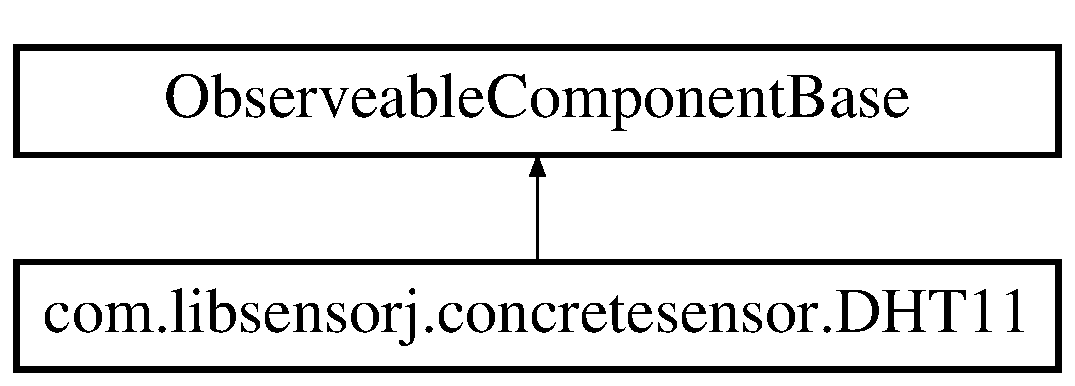
\includegraphics[height=2.000000cm]{classcom_1_1libsensorj_1_1concretesensor_1_1DHT11}
\end{center}
\end{figure}
\subsection*{Public Member Functions}
\begin{DoxyCompactItemize}
\item 
\hyperlink{classcom_1_1libsensorj_1_1concretesensor_1_1DHT11_a6dee6dabad63a5b8f8ba35f1279703c2}{D\+H\+T11} ()
\item 
\hyperlink{classcom_1_1libsensorj_1_1concretesensor_1_1DHT11_a6b867144169aa951ddbd09fc9ec5f6e5}{D\+H\+T11} (int pin)
\item 
double \hyperlink{classcom_1_1libsensorj_1_1concretesensor_1_1DHT11_a84f4c759756e582eb0e3d12675525c87}{read\+Value} ()
\item 
synchronized double \hyperlink{classcom_1_1libsensorj_1_1concretesensor_1_1DHT11_a4c88c53cbcacce861433ea2f03dd08f0}{get\+Temperature\+In\+Celsius} ()
\item 
synchronized double \hyperlink{classcom_1_1libsensorj_1_1concretesensor_1_1DHT11_a21bd2e0675b083a83610584d199c268b}{get\+Temperature\+In\+Fahrenheit} ()
\item 
synchronized double \hyperlink{classcom_1_1libsensorj_1_1concretesensor_1_1DHT11_ab2263c3d3e8deb1c1389fdb9c642b5ee}{get\+Temperature\+In\+Kelvin} ()
\end{DoxyCompactItemize}
\subsection*{Private Member Functions}
\begin{DoxyCompactItemize}
\item 
double \hyperlink{classcom_1_1libsensorj_1_1concretesensor_1_1DHT11_a1d452b9a4f3ff98d35cc425aee062bd4}{get\+Temperature} (Temperature\+Scale from)
\item 
boolean \hyperlink{classcom_1_1libsensorj_1_1concretesensor_1_1DHT11_a46fc1af81db68410209e81e5376428a9}{check\+Parity} ()
\end{DoxyCompactItemize}
\subsection*{Private Attributes}
\begin{DoxyCompactItemize}
\item 
int\mbox{[}$\,$\mbox{]} \hyperlink{classcom_1_1libsensorj_1_1concretesensor_1_1DHT11_a0d73b9b918bec661a7333f1f63e00d08}{dht11\+\_\+dat} = \{ 0, 0, 0, 0, 0 \}
\item 
Gpio\+Pin\+Digital\+Multipurpose \hyperlink{classcom_1_1libsensorj_1_1concretesensor_1_1DHT11_a816e6c7ffc2d313077cc5df4b2252b41}{dht11\+Pin}
\end{DoxyCompactItemize}
\subsection*{Static Private Attributes}
\begin{DoxyCompactItemize}
\item 
static final Pin \hyperlink{classcom_1_1libsensorj_1_1concretesensor_1_1DHT11_a90e62e8cc61299199eb1fa06bd441a9e}{D\+E\+F\+A\+U\+L\+T\+\_\+\+P\+I\+N} = Raspi\+Pin.\+G\+P\+I\+O\+\_\+04
\item 
static final int \hyperlink{classcom_1_1libsensorj_1_1concretesensor_1_1DHT11_ad986e37718b89038ff2702c80a2bb320}{M\+A\+X\+T\+I\+M\+I\+N\+G\+S} = 85
\item 
static final Logger \hyperlink{classcom_1_1libsensorj_1_1concretesensor_1_1DHT11_ad5b8d7e0ad34e4f3b28c081f259d1928}{L\+O\+G\+G\+E\+R}
\end{DoxyCompactItemize}


\subsection{Detailed Description}
The Class \hyperlink{classcom_1_1libsensorj_1_1concretesensor_1_1DHT11}{D\+H\+T11}. 

\subsection{Constructor \& Destructor Documentation}
\hypertarget{classcom_1_1libsensorj_1_1concretesensor_1_1DHT11_a6dee6dabad63a5b8f8ba35f1279703c2}{}\index{com\+::libsensorj\+::concretesensor\+::\+D\+H\+T11@{com\+::libsensorj\+::concretesensor\+::\+D\+H\+T11}!D\+H\+T11@{D\+H\+T11}}
\index{D\+H\+T11@{D\+H\+T11}!com\+::libsensorj\+::concretesensor\+::\+D\+H\+T11@{com\+::libsensorj\+::concretesensor\+::\+D\+H\+T11}}
\subsubsection[{D\+H\+T11}]{\setlength{\rightskip}{0pt plus 5cm}com.\+libsensorj.\+concretesensor.\+D\+H\+T11.\+D\+H\+T11 (
\begin{DoxyParamCaption}
{}
\end{DoxyParamCaption}
)}\label{classcom_1_1libsensorj_1_1concretesensor_1_1DHT11_a6dee6dabad63a5b8f8ba35f1279703c2}
Instantiates a new D\+Ht11. \hypertarget{classcom_1_1libsensorj_1_1concretesensor_1_1DHT11_a6b867144169aa951ddbd09fc9ec5f6e5}{}\index{com\+::libsensorj\+::concretesensor\+::\+D\+H\+T11@{com\+::libsensorj\+::concretesensor\+::\+D\+H\+T11}!D\+H\+T11@{D\+H\+T11}}
\index{D\+H\+T11@{D\+H\+T11}!com\+::libsensorj\+::concretesensor\+::\+D\+H\+T11@{com\+::libsensorj\+::concretesensor\+::\+D\+H\+T11}}
\subsubsection[{D\+H\+T11}]{\setlength{\rightskip}{0pt plus 5cm}com.\+libsensorj.\+concretesensor.\+D\+H\+T11.\+D\+H\+T11 (
\begin{DoxyParamCaption}
\item[{int}]{pin}
\end{DoxyParamCaption}
)}\label{classcom_1_1libsensorj_1_1concretesensor_1_1DHT11_a6b867144169aa951ddbd09fc9ec5f6e5}
Instantiates a new D\+Ht11.


\begin{DoxyParams}{Parameters}
{\em pin} & the pin \\
\hline
\end{DoxyParams}


\subsection{Member Function Documentation}
\hypertarget{classcom_1_1libsensorj_1_1concretesensor_1_1DHT11_a46fc1af81db68410209e81e5376428a9}{}\index{com\+::libsensorj\+::concretesensor\+::\+D\+H\+T11@{com\+::libsensorj\+::concretesensor\+::\+D\+H\+T11}!check\+Parity@{check\+Parity}}
\index{check\+Parity@{check\+Parity}!com\+::libsensorj\+::concretesensor\+::\+D\+H\+T11@{com\+::libsensorj\+::concretesensor\+::\+D\+H\+T11}}
\subsubsection[{check\+Parity}]{\setlength{\rightskip}{0pt plus 5cm}boolean com.\+libsensorj.\+concretesensor.\+D\+H\+T11.\+check\+Parity (
\begin{DoxyParamCaption}
{}
\end{DoxyParamCaption}
)\hspace{0.3cm}{\ttfamily [private]}}\label{classcom_1_1libsensorj_1_1concretesensor_1_1DHT11_a46fc1af81db68410209e81e5376428a9}
Check parity.

\begin{DoxyReturn}{Returns}
true, if successful 
\end{DoxyReturn}
\hypertarget{classcom_1_1libsensorj_1_1concretesensor_1_1DHT11_a1d452b9a4f3ff98d35cc425aee062bd4}{}\index{com\+::libsensorj\+::concretesensor\+::\+D\+H\+T11@{com\+::libsensorj\+::concretesensor\+::\+D\+H\+T11}!get\+Temperature@{get\+Temperature}}
\index{get\+Temperature@{get\+Temperature}!com\+::libsensorj\+::concretesensor\+::\+D\+H\+T11@{com\+::libsensorj\+::concretesensor\+::\+D\+H\+T11}}
\subsubsection[{get\+Temperature}]{\setlength{\rightskip}{0pt plus 5cm}double com.\+libsensorj.\+concretesensor.\+D\+H\+T11.\+get\+Temperature (
\begin{DoxyParamCaption}
\item[{Temperature\+Scale}]{from}
\end{DoxyParamCaption}
)\hspace{0.3cm}{\ttfamily [private]}}\label{classcom_1_1libsensorj_1_1concretesensor_1_1DHT11_a1d452b9a4f3ff98d35cc425aee062bd4}
Gets the temperature.


\begin{DoxyParams}{Parameters}
{\em from} & the Temperature\+Scale \\
\hline
\end{DoxyParams}
\begin{DoxyReturn}{Returns}
the temperature 
\end{DoxyReturn}
\hypertarget{classcom_1_1libsensorj_1_1concretesensor_1_1DHT11_a4c88c53cbcacce861433ea2f03dd08f0}{}\index{com\+::libsensorj\+::concretesensor\+::\+D\+H\+T11@{com\+::libsensorj\+::concretesensor\+::\+D\+H\+T11}!get\+Temperature\+In\+Celsius@{get\+Temperature\+In\+Celsius}}
\index{get\+Temperature\+In\+Celsius@{get\+Temperature\+In\+Celsius}!com\+::libsensorj\+::concretesensor\+::\+D\+H\+T11@{com\+::libsensorj\+::concretesensor\+::\+D\+H\+T11}}
\subsubsection[{get\+Temperature\+In\+Celsius}]{\setlength{\rightskip}{0pt plus 5cm}synchronized double com.\+libsensorj.\+concretesensor.\+D\+H\+T11.\+get\+Temperature\+In\+Celsius (
\begin{DoxyParamCaption}
{}
\end{DoxyParamCaption}
)}\label{classcom_1_1libsensorj_1_1concretesensor_1_1DHT11_a4c88c53cbcacce861433ea2f03dd08f0}
Gets the temperature in celsius.

\begin{DoxyReturn}{Returns}
the temperature in celsius 
\end{DoxyReturn}
\hypertarget{classcom_1_1libsensorj_1_1concretesensor_1_1DHT11_a21bd2e0675b083a83610584d199c268b}{}\index{com\+::libsensorj\+::concretesensor\+::\+D\+H\+T11@{com\+::libsensorj\+::concretesensor\+::\+D\+H\+T11}!get\+Temperature\+In\+Fahrenheit@{get\+Temperature\+In\+Fahrenheit}}
\index{get\+Temperature\+In\+Fahrenheit@{get\+Temperature\+In\+Fahrenheit}!com\+::libsensorj\+::concretesensor\+::\+D\+H\+T11@{com\+::libsensorj\+::concretesensor\+::\+D\+H\+T11}}
\subsubsection[{get\+Temperature\+In\+Fahrenheit}]{\setlength{\rightskip}{0pt plus 5cm}synchronized double com.\+libsensorj.\+concretesensor.\+D\+H\+T11.\+get\+Temperature\+In\+Fahrenheit (
\begin{DoxyParamCaption}
{}
\end{DoxyParamCaption}
)}\label{classcom_1_1libsensorj_1_1concretesensor_1_1DHT11_a21bd2e0675b083a83610584d199c268b}
Gets the temperature in fahrenheit.

\begin{DoxyReturn}{Returns}
the temperature in fahrenheit 
\end{DoxyReturn}
\hypertarget{classcom_1_1libsensorj_1_1concretesensor_1_1DHT11_ab2263c3d3e8deb1c1389fdb9c642b5ee}{}\index{com\+::libsensorj\+::concretesensor\+::\+D\+H\+T11@{com\+::libsensorj\+::concretesensor\+::\+D\+H\+T11}!get\+Temperature\+In\+Kelvin@{get\+Temperature\+In\+Kelvin}}
\index{get\+Temperature\+In\+Kelvin@{get\+Temperature\+In\+Kelvin}!com\+::libsensorj\+::concretesensor\+::\+D\+H\+T11@{com\+::libsensorj\+::concretesensor\+::\+D\+H\+T11}}
\subsubsection[{get\+Temperature\+In\+Kelvin}]{\setlength{\rightskip}{0pt plus 5cm}synchronized double com.\+libsensorj.\+concretesensor.\+D\+H\+T11.\+get\+Temperature\+In\+Kelvin (
\begin{DoxyParamCaption}
{}
\end{DoxyParamCaption}
)}\label{classcom_1_1libsensorj_1_1concretesensor_1_1DHT11_ab2263c3d3e8deb1c1389fdb9c642b5ee}
Gets the temperature in kelvin.

\begin{DoxyReturn}{Returns}
the temperature in kelvin 
\end{DoxyReturn}
\hypertarget{classcom_1_1libsensorj_1_1concretesensor_1_1DHT11_a84f4c759756e582eb0e3d12675525c87}{}\index{com\+::libsensorj\+::concretesensor\+::\+D\+H\+T11@{com\+::libsensorj\+::concretesensor\+::\+D\+H\+T11}!read\+Value@{read\+Value}}
\index{read\+Value@{read\+Value}!com\+::libsensorj\+::concretesensor\+::\+D\+H\+T11@{com\+::libsensorj\+::concretesensor\+::\+D\+H\+T11}}
\subsubsection[{read\+Value}]{\setlength{\rightskip}{0pt plus 5cm}double com.\+libsensorj.\+concretesensor.\+D\+H\+T11.\+read\+Value (
\begin{DoxyParamCaption}
{}
\end{DoxyParamCaption}
)}\label{classcom_1_1libsensorj_1_1concretesensor_1_1DHT11_a84f4c759756e582eb0e3d12675525c87}
Read value.

\begin{DoxyReturn}{Returns}
the value readed 
\end{DoxyReturn}


\subsection{Member Data Documentation}
\hypertarget{classcom_1_1libsensorj_1_1concretesensor_1_1DHT11_a90e62e8cc61299199eb1fa06bd441a9e}{}\index{com\+::libsensorj\+::concretesensor\+::\+D\+H\+T11@{com\+::libsensorj\+::concretesensor\+::\+D\+H\+T11}!D\+E\+F\+A\+U\+L\+T\+\_\+\+P\+I\+N@{D\+E\+F\+A\+U\+L\+T\+\_\+\+P\+I\+N}}
\index{D\+E\+F\+A\+U\+L\+T\+\_\+\+P\+I\+N@{D\+E\+F\+A\+U\+L\+T\+\_\+\+P\+I\+N}!com\+::libsensorj\+::concretesensor\+::\+D\+H\+T11@{com\+::libsensorj\+::concretesensor\+::\+D\+H\+T11}}
\subsubsection[{D\+E\+F\+A\+U\+L\+T\+\_\+\+P\+I\+N}]{\setlength{\rightskip}{0pt plus 5cm}final Pin com.\+libsensorj.\+concretesensor.\+D\+H\+T11.\+D\+E\+F\+A\+U\+L\+T\+\_\+\+P\+I\+N = Raspi\+Pin.\+G\+P\+I\+O\+\_\+04\hspace{0.3cm}{\ttfamily [static]}, {\ttfamily [private]}}\label{classcom_1_1libsensorj_1_1concretesensor_1_1DHT11_a90e62e8cc61299199eb1fa06bd441a9e}
The Constant D\+E\+F\+A\+U\+L\+T\+\_\+\+P\+I\+N. \hypertarget{classcom_1_1libsensorj_1_1concretesensor_1_1DHT11_a0d73b9b918bec661a7333f1f63e00d08}{}\index{com\+::libsensorj\+::concretesensor\+::\+D\+H\+T11@{com\+::libsensorj\+::concretesensor\+::\+D\+H\+T11}!dht11\+\_\+dat@{dht11\+\_\+dat}}
\index{dht11\+\_\+dat@{dht11\+\_\+dat}!com\+::libsensorj\+::concretesensor\+::\+D\+H\+T11@{com\+::libsensorj\+::concretesensor\+::\+D\+H\+T11}}
\subsubsection[{dht11\+\_\+dat}]{\setlength{\rightskip}{0pt plus 5cm}int \mbox{[}$\,$\mbox{]} com.\+libsensorj.\+concretesensor.\+D\+H\+T11.\+dht11\+\_\+dat = \{ 0, 0, 0, 0, 0 \}\hspace{0.3cm}{\ttfamily [private]}}\label{classcom_1_1libsensorj_1_1concretesensor_1_1DHT11_a0d73b9b918bec661a7333f1f63e00d08}
The dht11\+\_\+dat. \hypertarget{classcom_1_1libsensorj_1_1concretesensor_1_1DHT11_a816e6c7ffc2d313077cc5df4b2252b41}{}\index{com\+::libsensorj\+::concretesensor\+::\+D\+H\+T11@{com\+::libsensorj\+::concretesensor\+::\+D\+H\+T11}!dht11\+Pin@{dht11\+Pin}}
\index{dht11\+Pin@{dht11\+Pin}!com\+::libsensorj\+::concretesensor\+::\+D\+H\+T11@{com\+::libsensorj\+::concretesensor\+::\+D\+H\+T11}}
\subsubsection[{dht11\+Pin}]{\setlength{\rightskip}{0pt plus 5cm}Gpio\+Pin\+Digital\+Multipurpose com.\+libsensorj.\+concretesensor.\+D\+H\+T11.\+dht11\+Pin\hspace{0.3cm}{\ttfamily [private]}}\label{classcom_1_1libsensorj_1_1concretesensor_1_1DHT11_a816e6c7ffc2d313077cc5df4b2252b41}
The dht11 pin. \hypertarget{classcom_1_1libsensorj_1_1concretesensor_1_1DHT11_ad5b8d7e0ad34e4f3b28c081f259d1928}{}\index{com\+::libsensorj\+::concretesensor\+::\+D\+H\+T11@{com\+::libsensorj\+::concretesensor\+::\+D\+H\+T11}!L\+O\+G\+G\+E\+R@{L\+O\+G\+G\+E\+R}}
\index{L\+O\+G\+G\+E\+R@{L\+O\+G\+G\+E\+R}!com\+::libsensorj\+::concretesensor\+::\+D\+H\+T11@{com\+::libsensorj\+::concretesensor\+::\+D\+H\+T11}}
\subsubsection[{L\+O\+G\+G\+E\+R}]{\setlength{\rightskip}{0pt plus 5cm}final Logger com.\+libsensorj.\+concretesensor.\+D\+H\+T11.\+L\+O\+G\+G\+E\+R\hspace{0.3cm}{\ttfamily [static]}, {\ttfamily [private]}}\label{classcom_1_1libsensorj_1_1concretesensor_1_1DHT11_ad5b8d7e0ad34e4f3b28c081f259d1928}
{\bfseries Initial value\+:}
\begin{DoxyCode}
= LogManager.getLogger(\hyperlink{classcom_1_1libsensorj_1_1concretesensor_1_1DHT11_a6dee6dabad63a5b8f8ba35f1279703c2}{DHT11}.class
            .getName())
\end{DoxyCode}
The Constant L\+O\+G\+G\+E\+R. \hypertarget{classcom_1_1libsensorj_1_1concretesensor_1_1DHT11_ad986e37718b89038ff2702c80a2bb320}{}\index{com\+::libsensorj\+::concretesensor\+::\+D\+H\+T11@{com\+::libsensorj\+::concretesensor\+::\+D\+H\+T11}!M\+A\+X\+T\+I\+M\+I\+N\+G\+S@{M\+A\+X\+T\+I\+M\+I\+N\+G\+S}}
\index{M\+A\+X\+T\+I\+M\+I\+N\+G\+S@{M\+A\+X\+T\+I\+M\+I\+N\+G\+S}!com\+::libsensorj\+::concretesensor\+::\+D\+H\+T11@{com\+::libsensorj\+::concretesensor\+::\+D\+H\+T11}}
\subsubsection[{M\+A\+X\+T\+I\+M\+I\+N\+G\+S}]{\setlength{\rightskip}{0pt plus 5cm}final int com.\+libsensorj.\+concretesensor.\+D\+H\+T11.\+M\+A\+X\+T\+I\+M\+I\+N\+G\+S = 85\hspace{0.3cm}{\ttfamily [static]}, {\ttfamily [private]}}\label{classcom_1_1libsensorj_1_1concretesensor_1_1DHT11_ad986e37718b89038ff2702c80a2bb320}
The Constant M\+A\+X\+T\+I\+M\+I\+N\+G\+S. 

The documentation for this class was generated from the following file\+:\begin{DoxyCompactItemize}
\item 
main/java/com/libsensorj/concretesensor/\hyperlink{DHT11_8java}{D\+H\+T11.\+java}\end{DoxyCompactItemize}

\hypertarget{classcom_1_1libsensorj_1_1concretesensor_1_1DHT11Humidity}{}\section{com.\+libsensorj.\+concretesensor.\+D\+H\+T11\+Humidity Class Reference}
\label{classcom_1_1libsensorj_1_1concretesensor_1_1DHT11Humidity}\index{com.\+libsensorj.\+concretesensor.\+D\+H\+T11\+Humidity@{com.\+libsensorj.\+concretesensor.\+D\+H\+T11\+Humidity}}
Inheritance diagram for com.\+libsensorj.\+concretesensor.\+D\+H\+T11\+Humidity\+:\begin{figure}[H]
\begin{center}
\leavevmode
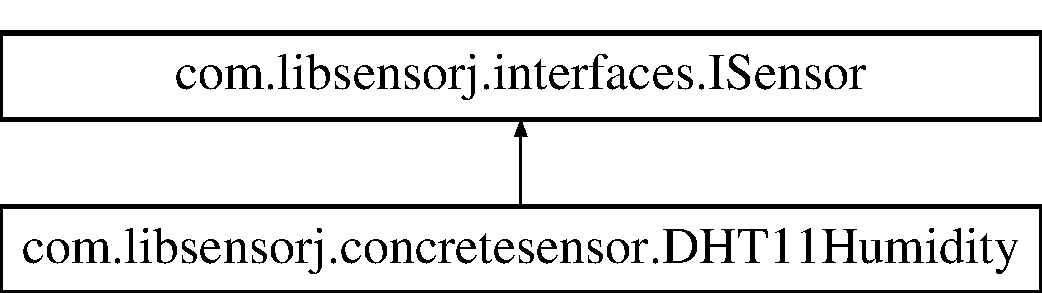
\includegraphics[height=2.000000cm]{classcom_1_1libsensorj_1_1concretesensor_1_1DHT11Humidity}
\end{center}
\end{figure}
\subsection*{Public Member Functions}
\begin{DoxyCompactItemize}
\item 
void \hyperlink{classcom_1_1libsensorj_1_1concretesensor_1_1DHT11Humidity_a2355dc003abad8d519440e9f6871c422}{get\+Instance} ()
\end{DoxyCompactItemize}
\subsection*{Static Private Attributes}
\begin{DoxyCompactItemize}
\item 
static final Logger \hyperlink{classcom_1_1libsensorj_1_1concretesensor_1_1DHT11Humidity_a80655575ba16db014b7a1a797e030eae}{L\+O\+G\+G\+E\+R}
\end{DoxyCompactItemize}


\subsection{Detailed Description}
The Class \hyperlink{classcom_1_1libsensorj_1_1concretesensor_1_1DHT11Humidity}{D\+H\+T11\+Humidity}. 

\subsection{Member Function Documentation}
\hypertarget{classcom_1_1libsensorj_1_1concretesensor_1_1DHT11Humidity_a2355dc003abad8d519440e9f6871c422}{}\index{com\+::libsensorj\+::concretesensor\+::\+D\+H\+T11\+Humidity@{com\+::libsensorj\+::concretesensor\+::\+D\+H\+T11\+Humidity}!get\+Instance@{get\+Instance}}
\index{get\+Instance@{get\+Instance}!com\+::libsensorj\+::concretesensor\+::\+D\+H\+T11\+Humidity@{com\+::libsensorj\+::concretesensor\+::\+D\+H\+T11\+Humidity}}
\subsubsection[{get\+Instance}]{\setlength{\rightskip}{0pt plus 5cm}void com.\+libsensorj.\+concretesensor.\+D\+H\+T11\+Humidity.\+get\+Instance (
\begin{DoxyParamCaption}
{}
\end{DoxyParamCaption}
)}\label{classcom_1_1libsensorj_1_1concretesensor_1_1DHT11Humidity_a2355dc003abad8d519440e9f6871c422}
Gets the single instance of I\+Sensor.

\begin{DoxyReturn}{Returns}
single instance of I\+Sensor 
\end{DoxyReturn}


Implements \hyperlink{interfacecom_1_1libsensorj_1_1interfaces_1_1ISensor_a3c3db93a33adecde81a528651790f75e}{com.\+libsensorj.\+interfaces.\+I\+Sensor}.



\subsection{Member Data Documentation}
\hypertarget{classcom_1_1libsensorj_1_1concretesensor_1_1DHT11Humidity_a80655575ba16db014b7a1a797e030eae}{}\index{com\+::libsensorj\+::concretesensor\+::\+D\+H\+T11\+Humidity@{com\+::libsensorj\+::concretesensor\+::\+D\+H\+T11\+Humidity}!L\+O\+G\+G\+E\+R@{L\+O\+G\+G\+E\+R}}
\index{L\+O\+G\+G\+E\+R@{L\+O\+G\+G\+E\+R}!com\+::libsensorj\+::concretesensor\+::\+D\+H\+T11\+Humidity@{com\+::libsensorj\+::concretesensor\+::\+D\+H\+T11\+Humidity}}
\subsubsection[{L\+O\+G\+G\+E\+R}]{\setlength{\rightskip}{0pt plus 5cm}final Logger com.\+libsensorj.\+concretesensor.\+D\+H\+T11\+Humidity.\+L\+O\+G\+G\+E\+R\hspace{0.3cm}{\ttfamily [static]}, {\ttfamily [private]}}\label{classcom_1_1libsensorj_1_1concretesensor_1_1DHT11Humidity_a80655575ba16db014b7a1a797e030eae}
{\bfseries Initial value\+:}
\begin{DoxyCode}
= LogManager
            .getLogger(DHT11Humidity.class.getName())
\end{DoxyCode}
The Constant L\+O\+G\+G\+E\+R. 

The documentation for this class was generated from the following file\+:\begin{DoxyCompactItemize}
\item 
main/java/com/libsensorj/concretesensor/\hyperlink{DHT11Humidity_8java}{D\+H\+T11\+Humidity.\+java}\end{DoxyCompactItemize}

\hypertarget{classcom_1_1libsensorj_1_1concretesensor_1_1DHT11Temperature}{}\section{com.\+libsensorj.\+concretesensor.\+D\+H\+T11\+Temperature Class Reference}
\label{classcom_1_1libsensorj_1_1concretesensor_1_1DHT11Temperature}\index{com.\+libsensorj.\+concretesensor.\+D\+H\+T11\+Temperature@{com.\+libsensorj.\+concretesensor.\+D\+H\+T11\+Temperature}}
Inheritance diagram for com.\+libsensorj.\+concretesensor.\+D\+H\+T11\+Temperature\+:\begin{figure}[H]
\begin{center}
\leavevmode
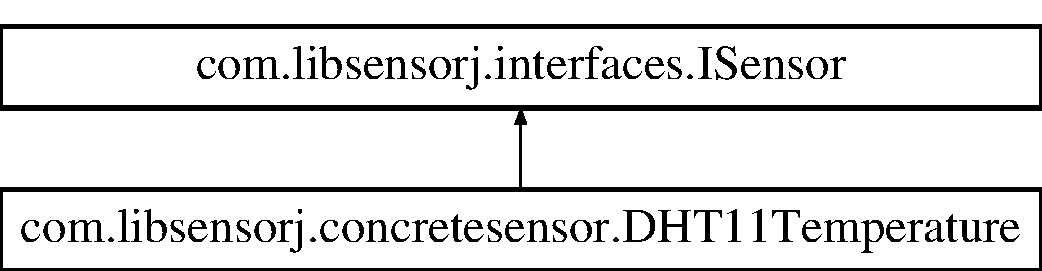
\includegraphics[height=2.000000cm]{classcom_1_1libsensorj_1_1concretesensor_1_1DHT11Temperature}
\end{center}
\end{figure}
\subsection*{Public Member Functions}
\begin{DoxyCompactItemize}
\item 
\hyperlink{classcom_1_1libsensorj_1_1concretesensor_1_1DHT11Temperature_a81324fa18ad12062d493a880f3fbda67}{D\+H\+T11\+Temperature} (int \hyperlink{classcom_1_1libsensorj_1_1concretesensor_1_1DHT11Temperature_a312572f2f0bad8b41d171481ef4e3138}{gpio\+Pin})
\item 
\hyperlink{classcom_1_1libsensorj_1_1concretesensor_1_1DHT11Temperature_a02bbdf30c922adcbde84597bf698ff41}{D\+H\+T11\+Temperature} ()
\item 
void \hyperlink{classcom_1_1libsensorj_1_1concretesensor_1_1DHT11Temperature_a599358623598fb0076dc0a2e07978f0b}{get\+Instance} ()
\item 
synchronized double \hyperlink{classcom_1_1libsensorj_1_1concretesensor_1_1DHT11Temperature_ab0b6a73583d9244271174a3d896f5ed3}{get\+Temperature\+In\+Celsius} ()
\item 
synchronized double \hyperlink{classcom_1_1libsensorj_1_1concretesensor_1_1DHT11Temperature_aa564f9c66609426711cbd0fbfe6837e3}{get\+Temperature\+In\+Fahrenheit} ()
\item 
synchronized double \hyperlink{classcom_1_1libsensorj_1_1concretesensor_1_1DHT11Temperature_a2c1a2bfaaf97612a862079979394ff34}{get\+Temperature\+In\+Kelvin} ()
\end{DoxyCompactItemize}
\subsection*{Private Member Functions}
\begin{DoxyCompactItemize}
\item 
void \hyperlink{classcom_1_1libsensorj_1_1concretesensor_1_1DHT11Temperature_a0ed494577e6a3c68dc737b60f926269d}{check\+For\+Updates} ()
\item 
double \hyperlink{classcom_1_1libsensorj_1_1concretesensor_1_1DHT11Temperature_abb836186013ae429e2cfde981154969b}{get\+Temperature} (Temperature\+Scale from)
\item 
double \hyperlink{classcom_1_1libsensorj_1_1concretesensor_1_1DHT11Temperature_a061220e6439c2014ab81384738c07734}{parse\+Temperature} (String value)
\item 
String \hyperlink{classcom_1_1libsensorj_1_1concretesensor_1_1DHT11Temperature_a2e5125c490d1b7b28a359cf702334fd7}{read\+Values} ()
\end{DoxyCompactItemize}
\subsection*{Private Attributes}
\begin{DoxyCompactItemize}
\item 
String \hyperlink{classcom_1_1libsensorj_1_1concretesensor_1_1DHT11Temperature_af16dd6a4c88dedacb8a4d69d90eff670}{last\+Value}
\item 
long \hyperlink{classcom_1_1libsensorj_1_1concretesensor_1_1DHT11Temperature_a00ec2e3e31bcaf04f497d5c503a84c5e}{last\+Check}
\item 
final int \hyperlink{classcom_1_1libsensorj_1_1concretesensor_1_1DHT11Temperature_a312572f2f0bad8b41d171481ef4e3138}{gpio\+Pin}
\end{DoxyCompactItemize}
\subsection*{Static Private Attributes}
\begin{DoxyCompactItemize}
\item 
static final String \hyperlink{classcom_1_1libsensorj_1_1concretesensor_1_1DHT11Temperature_a123ae6845e0cc1d1ec859cf7cfb78004}{T\+E\+M\+P\+\_\+\+S\+T\+R} = \char`\"{}Temp =\char`\"{}
\item 
static final int \hyperlink{classcom_1_1libsensorj_1_1concretesensor_1_1DHT11Temperature_af8bf5091500d4dcb3b5a0663279359e2}{D\+E\+F\+A\+U\+L\+T\+\_\+\+P\+I\+N} = 4
\item 
static final long \hyperlink{classcom_1_1libsensorj_1_1concretesensor_1_1DHT11Temperature_a7a5b6b6685407c05809a7e4c97358dd4}{L\+A\+S\+T\+\_\+\+C\+H\+E\+C\+K\+\_\+\+D\+I\+F\+F} = 3000
\item 
static final Logger \hyperlink{classcom_1_1libsensorj_1_1concretesensor_1_1DHT11Temperature_a96d485fc09496c1b5a320a30bb3400c9}{L\+O\+G\+G\+E\+R}
\end{DoxyCompactItemize}


\subsection{Detailed Description}
The Class \hyperlink{classcom_1_1libsensorj_1_1concretesensor_1_1DHT11Temperature}{D\+H\+T11\+Temperature}. 

\subsection{Constructor \& Destructor Documentation}
\hypertarget{classcom_1_1libsensorj_1_1concretesensor_1_1DHT11Temperature_a81324fa18ad12062d493a880f3fbda67}{}\index{com\+::libsensorj\+::concretesensor\+::\+D\+H\+T11\+Temperature@{com\+::libsensorj\+::concretesensor\+::\+D\+H\+T11\+Temperature}!D\+H\+T11\+Temperature@{D\+H\+T11\+Temperature}}
\index{D\+H\+T11\+Temperature@{D\+H\+T11\+Temperature}!com\+::libsensorj\+::concretesensor\+::\+D\+H\+T11\+Temperature@{com\+::libsensorj\+::concretesensor\+::\+D\+H\+T11\+Temperature}}
\subsubsection[{D\+H\+T11\+Temperature}]{\setlength{\rightskip}{0pt plus 5cm}com.\+libsensorj.\+concretesensor.\+D\+H\+T11\+Temperature.\+D\+H\+T11\+Temperature (
\begin{DoxyParamCaption}
\item[{int}]{gpio\+Pin}
\end{DoxyParamCaption}
)}\label{classcom_1_1libsensorj_1_1concretesensor_1_1DHT11Temperature_a81324fa18ad12062d493a880f3fbda67}
Instantiates a new D\+Ht11 temperature.


\begin{DoxyParams}{Parameters}
{\em gpio\+Pin} & the gpio pin \\
\hline
\end{DoxyParams}
\hypertarget{classcom_1_1libsensorj_1_1concretesensor_1_1DHT11Temperature_a02bbdf30c922adcbde84597bf698ff41}{}\index{com\+::libsensorj\+::concretesensor\+::\+D\+H\+T11\+Temperature@{com\+::libsensorj\+::concretesensor\+::\+D\+H\+T11\+Temperature}!D\+H\+T11\+Temperature@{D\+H\+T11\+Temperature}}
\index{D\+H\+T11\+Temperature@{D\+H\+T11\+Temperature}!com\+::libsensorj\+::concretesensor\+::\+D\+H\+T11\+Temperature@{com\+::libsensorj\+::concretesensor\+::\+D\+H\+T11\+Temperature}}
\subsubsection[{D\+H\+T11\+Temperature}]{\setlength{\rightskip}{0pt plus 5cm}com.\+libsensorj.\+concretesensor.\+D\+H\+T11\+Temperature.\+D\+H\+T11\+Temperature (
\begin{DoxyParamCaption}
{}
\end{DoxyParamCaption}
)}\label{classcom_1_1libsensorj_1_1concretesensor_1_1DHT11Temperature_a02bbdf30c922adcbde84597bf698ff41}
Instantiates a new D\+Ht11 temperature. 

\subsection{Member Function Documentation}
\hypertarget{classcom_1_1libsensorj_1_1concretesensor_1_1DHT11Temperature_a0ed494577e6a3c68dc737b60f926269d}{}\index{com\+::libsensorj\+::concretesensor\+::\+D\+H\+T11\+Temperature@{com\+::libsensorj\+::concretesensor\+::\+D\+H\+T11\+Temperature}!check\+For\+Updates@{check\+For\+Updates}}
\index{check\+For\+Updates@{check\+For\+Updates}!com\+::libsensorj\+::concretesensor\+::\+D\+H\+T11\+Temperature@{com\+::libsensorj\+::concretesensor\+::\+D\+H\+T11\+Temperature}}
\subsubsection[{check\+For\+Updates}]{\setlength{\rightskip}{0pt plus 5cm}void com.\+libsensorj.\+concretesensor.\+D\+H\+T11\+Temperature.\+check\+For\+Updates (
\begin{DoxyParamCaption}
{}
\end{DoxyParamCaption}
)\hspace{0.3cm}{\ttfamily [private]}}\label{classcom_1_1libsensorj_1_1concretesensor_1_1DHT11Temperature_a0ed494577e6a3c68dc737b60f926269d}
Check for updates. \hypertarget{classcom_1_1libsensorj_1_1concretesensor_1_1DHT11Temperature_a599358623598fb0076dc0a2e07978f0b}{}\index{com\+::libsensorj\+::concretesensor\+::\+D\+H\+T11\+Temperature@{com\+::libsensorj\+::concretesensor\+::\+D\+H\+T11\+Temperature}!get\+Instance@{get\+Instance}}
\index{get\+Instance@{get\+Instance}!com\+::libsensorj\+::concretesensor\+::\+D\+H\+T11\+Temperature@{com\+::libsensorj\+::concretesensor\+::\+D\+H\+T11\+Temperature}}
\subsubsection[{get\+Instance}]{\setlength{\rightskip}{0pt plus 5cm}void com.\+libsensorj.\+concretesensor.\+D\+H\+T11\+Temperature.\+get\+Instance (
\begin{DoxyParamCaption}
{}
\end{DoxyParamCaption}
)}\label{classcom_1_1libsensorj_1_1concretesensor_1_1DHT11Temperature_a599358623598fb0076dc0a2e07978f0b}
Gets the single instance of I\+Sensor.

\begin{DoxyReturn}{Returns}
single instance of I\+Sensor 
\end{DoxyReturn}


Implements \hyperlink{interfacecom_1_1libsensorj_1_1interfaces_1_1ISensor_a3c3db93a33adecde81a528651790f75e}{com.\+libsensorj.\+interfaces.\+I\+Sensor}.

\hypertarget{classcom_1_1libsensorj_1_1concretesensor_1_1DHT11Temperature_abb836186013ae429e2cfde981154969b}{}\index{com\+::libsensorj\+::concretesensor\+::\+D\+H\+T11\+Temperature@{com\+::libsensorj\+::concretesensor\+::\+D\+H\+T11\+Temperature}!get\+Temperature@{get\+Temperature}}
\index{get\+Temperature@{get\+Temperature}!com\+::libsensorj\+::concretesensor\+::\+D\+H\+T11\+Temperature@{com\+::libsensorj\+::concretesensor\+::\+D\+H\+T11\+Temperature}}
\subsubsection[{get\+Temperature}]{\setlength{\rightskip}{0pt plus 5cm}double com.\+libsensorj.\+concretesensor.\+D\+H\+T11\+Temperature.\+get\+Temperature (
\begin{DoxyParamCaption}
\item[{Temperature\+Scale}]{from}
\end{DoxyParamCaption}
)\hspace{0.3cm}{\ttfamily [private]}}\label{classcom_1_1libsensorj_1_1concretesensor_1_1DHT11Temperature_abb836186013ae429e2cfde981154969b}
Gets the temperature.


\begin{DoxyParams}{Parameters}
{\em from} & the from \\
\hline
\end{DoxyParams}
\begin{DoxyReturn}{Returns}
the temperature 
\end{DoxyReturn}
\hypertarget{classcom_1_1libsensorj_1_1concretesensor_1_1DHT11Temperature_ab0b6a73583d9244271174a3d896f5ed3}{}\index{com\+::libsensorj\+::concretesensor\+::\+D\+H\+T11\+Temperature@{com\+::libsensorj\+::concretesensor\+::\+D\+H\+T11\+Temperature}!get\+Temperature\+In\+Celsius@{get\+Temperature\+In\+Celsius}}
\index{get\+Temperature\+In\+Celsius@{get\+Temperature\+In\+Celsius}!com\+::libsensorj\+::concretesensor\+::\+D\+H\+T11\+Temperature@{com\+::libsensorj\+::concretesensor\+::\+D\+H\+T11\+Temperature}}
\subsubsection[{get\+Temperature\+In\+Celsius}]{\setlength{\rightskip}{0pt plus 5cm}synchronized double com.\+libsensorj.\+concretesensor.\+D\+H\+T11\+Temperature.\+get\+Temperature\+In\+Celsius (
\begin{DoxyParamCaption}
{}
\end{DoxyParamCaption}
)}\label{classcom_1_1libsensorj_1_1concretesensor_1_1DHT11Temperature_ab0b6a73583d9244271174a3d896f5ed3}
Gets the temperature in celsius.

\begin{DoxyReturn}{Returns}
the temperature in celsius 
\end{DoxyReturn}
\hypertarget{classcom_1_1libsensorj_1_1concretesensor_1_1DHT11Temperature_aa564f9c66609426711cbd0fbfe6837e3}{}\index{com\+::libsensorj\+::concretesensor\+::\+D\+H\+T11\+Temperature@{com\+::libsensorj\+::concretesensor\+::\+D\+H\+T11\+Temperature}!get\+Temperature\+In\+Fahrenheit@{get\+Temperature\+In\+Fahrenheit}}
\index{get\+Temperature\+In\+Fahrenheit@{get\+Temperature\+In\+Fahrenheit}!com\+::libsensorj\+::concretesensor\+::\+D\+H\+T11\+Temperature@{com\+::libsensorj\+::concretesensor\+::\+D\+H\+T11\+Temperature}}
\subsubsection[{get\+Temperature\+In\+Fahrenheit}]{\setlength{\rightskip}{0pt plus 5cm}synchronized double com.\+libsensorj.\+concretesensor.\+D\+H\+T11\+Temperature.\+get\+Temperature\+In\+Fahrenheit (
\begin{DoxyParamCaption}
{}
\end{DoxyParamCaption}
)}\label{classcom_1_1libsensorj_1_1concretesensor_1_1DHT11Temperature_aa564f9c66609426711cbd0fbfe6837e3}
Gets the temperature in fahrenheit.

\begin{DoxyReturn}{Returns}
the temperature in fahrenheit 
\end{DoxyReturn}
\hypertarget{classcom_1_1libsensorj_1_1concretesensor_1_1DHT11Temperature_a2c1a2bfaaf97612a862079979394ff34}{}\index{com\+::libsensorj\+::concretesensor\+::\+D\+H\+T11\+Temperature@{com\+::libsensorj\+::concretesensor\+::\+D\+H\+T11\+Temperature}!get\+Temperature\+In\+Kelvin@{get\+Temperature\+In\+Kelvin}}
\index{get\+Temperature\+In\+Kelvin@{get\+Temperature\+In\+Kelvin}!com\+::libsensorj\+::concretesensor\+::\+D\+H\+T11\+Temperature@{com\+::libsensorj\+::concretesensor\+::\+D\+H\+T11\+Temperature}}
\subsubsection[{get\+Temperature\+In\+Kelvin}]{\setlength{\rightskip}{0pt plus 5cm}synchronized double com.\+libsensorj.\+concretesensor.\+D\+H\+T11\+Temperature.\+get\+Temperature\+In\+Kelvin (
\begin{DoxyParamCaption}
{}
\end{DoxyParamCaption}
)}\label{classcom_1_1libsensorj_1_1concretesensor_1_1DHT11Temperature_a2c1a2bfaaf97612a862079979394ff34}
Gets the temperature in kelvin.

\begin{DoxyReturn}{Returns}
the temperature in kelvin 
\end{DoxyReturn}
\hypertarget{classcom_1_1libsensorj_1_1concretesensor_1_1DHT11Temperature_a061220e6439c2014ab81384738c07734}{}\index{com\+::libsensorj\+::concretesensor\+::\+D\+H\+T11\+Temperature@{com\+::libsensorj\+::concretesensor\+::\+D\+H\+T11\+Temperature}!parse\+Temperature@{parse\+Temperature}}
\index{parse\+Temperature@{parse\+Temperature}!com\+::libsensorj\+::concretesensor\+::\+D\+H\+T11\+Temperature@{com\+::libsensorj\+::concretesensor\+::\+D\+H\+T11\+Temperature}}
\subsubsection[{parse\+Temperature}]{\setlength{\rightskip}{0pt plus 5cm}double com.\+libsensorj.\+concretesensor.\+D\+H\+T11\+Temperature.\+parse\+Temperature (
\begin{DoxyParamCaption}
\item[{String}]{value}
\end{DoxyParamCaption}
)\hspace{0.3cm}{\ttfamily [private]}}\label{classcom_1_1libsensorj_1_1concretesensor_1_1DHT11Temperature_a061220e6439c2014ab81384738c07734}
Parses the temperature.


\begin{DoxyParams}{Parameters}
{\em value} & the value \\
\hline
\end{DoxyParams}
\begin{DoxyReturn}{Returns}
the double 
\end{DoxyReturn}
\hypertarget{classcom_1_1libsensorj_1_1concretesensor_1_1DHT11Temperature_a2e5125c490d1b7b28a359cf702334fd7}{}\index{com\+::libsensorj\+::concretesensor\+::\+D\+H\+T11\+Temperature@{com\+::libsensorj\+::concretesensor\+::\+D\+H\+T11\+Temperature}!read\+Values@{read\+Values}}
\index{read\+Values@{read\+Values}!com\+::libsensorj\+::concretesensor\+::\+D\+H\+T11\+Temperature@{com\+::libsensorj\+::concretesensor\+::\+D\+H\+T11\+Temperature}}
\subsubsection[{read\+Values}]{\setlength{\rightskip}{0pt plus 5cm}String com.\+libsensorj.\+concretesensor.\+D\+H\+T11\+Temperature.\+read\+Values (
\begin{DoxyParamCaption}
{}
\end{DoxyParamCaption}
)\hspace{0.3cm}{\ttfamily [private]}}\label{classcom_1_1libsensorj_1_1concretesensor_1_1DHT11Temperature_a2e5125c490d1b7b28a359cf702334fd7}
Read values.

\begin{DoxyReturn}{Returns}
the value readed as a string 
\end{DoxyReturn}


\subsection{Member Data Documentation}
\hypertarget{classcom_1_1libsensorj_1_1concretesensor_1_1DHT11Temperature_af8bf5091500d4dcb3b5a0663279359e2}{}\index{com\+::libsensorj\+::concretesensor\+::\+D\+H\+T11\+Temperature@{com\+::libsensorj\+::concretesensor\+::\+D\+H\+T11\+Temperature}!D\+E\+F\+A\+U\+L\+T\+\_\+\+P\+I\+N@{D\+E\+F\+A\+U\+L\+T\+\_\+\+P\+I\+N}}
\index{D\+E\+F\+A\+U\+L\+T\+\_\+\+P\+I\+N@{D\+E\+F\+A\+U\+L\+T\+\_\+\+P\+I\+N}!com\+::libsensorj\+::concretesensor\+::\+D\+H\+T11\+Temperature@{com\+::libsensorj\+::concretesensor\+::\+D\+H\+T11\+Temperature}}
\subsubsection[{D\+E\+F\+A\+U\+L\+T\+\_\+\+P\+I\+N}]{\setlength{\rightskip}{0pt plus 5cm}final int com.\+libsensorj.\+concretesensor.\+D\+H\+T11\+Temperature.\+D\+E\+F\+A\+U\+L\+T\+\_\+\+P\+I\+N = 4\hspace{0.3cm}{\ttfamily [static]}, {\ttfamily [private]}}\label{classcom_1_1libsensorj_1_1concretesensor_1_1DHT11Temperature_af8bf5091500d4dcb3b5a0663279359e2}
The Constant D\+E\+F\+A\+U\+L\+T\+\_\+\+P\+I\+N. \hypertarget{classcom_1_1libsensorj_1_1concretesensor_1_1DHT11Temperature_a312572f2f0bad8b41d171481ef4e3138}{}\index{com\+::libsensorj\+::concretesensor\+::\+D\+H\+T11\+Temperature@{com\+::libsensorj\+::concretesensor\+::\+D\+H\+T11\+Temperature}!gpio\+Pin@{gpio\+Pin}}
\index{gpio\+Pin@{gpio\+Pin}!com\+::libsensorj\+::concretesensor\+::\+D\+H\+T11\+Temperature@{com\+::libsensorj\+::concretesensor\+::\+D\+H\+T11\+Temperature}}
\subsubsection[{gpio\+Pin}]{\setlength{\rightskip}{0pt plus 5cm}final int com.\+libsensorj.\+concretesensor.\+D\+H\+T11\+Temperature.\+gpio\+Pin\hspace{0.3cm}{\ttfamily [private]}}\label{classcom_1_1libsensorj_1_1concretesensor_1_1DHT11Temperature_a312572f2f0bad8b41d171481ef4e3138}
The gpio pin. \hypertarget{classcom_1_1libsensorj_1_1concretesensor_1_1DHT11Temperature_a7a5b6b6685407c05809a7e4c97358dd4}{}\index{com\+::libsensorj\+::concretesensor\+::\+D\+H\+T11\+Temperature@{com\+::libsensorj\+::concretesensor\+::\+D\+H\+T11\+Temperature}!L\+A\+S\+T\+\_\+\+C\+H\+E\+C\+K\+\_\+\+D\+I\+F\+F@{L\+A\+S\+T\+\_\+\+C\+H\+E\+C\+K\+\_\+\+D\+I\+F\+F}}
\index{L\+A\+S\+T\+\_\+\+C\+H\+E\+C\+K\+\_\+\+D\+I\+F\+F@{L\+A\+S\+T\+\_\+\+C\+H\+E\+C\+K\+\_\+\+D\+I\+F\+F}!com\+::libsensorj\+::concretesensor\+::\+D\+H\+T11\+Temperature@{com\+::libsensorj\+::concretesensor\+::\+D\+H\+T11\+Temperature}}
\subsubsection[{L\+A\+S\+T\+\_\+\+C\+H\+E\+C\+K\+\_\+\+D\+I\+F\+F}]{\setlength{\rightskip}{0pt plus 5cm}final long com.\+libsensorj.\+concretesensor.\+D\+H\+T11\+Temperature.\+L\+A\+S\+T\+\_\+\+C\+H\+E\+C\+K\+\_\+\+D\+I\+F\+F = 3000\hspace{0.3cm}{\ttfamily [static]}, {\ttfamily [private]}}\label{classcom_1_1libsensorj_1_1concretesensor_1_1DHT11Temperature_a7a5b6b6685407c05809a7e4c97358dd4}
The Constant L\+A\+S\+T\+\_\+\+C\+H\+E\+C\+K\+\_\+\+D\+I\+F\+F. \hypertarget{classcom_1_1libsensorj_1_1concretesensor_1_1DHT11Temperature_a00ec2e3e31bcaf04f497d5c503a84c5e}{}\index{com\+::libsensorj\+::concretesensor\+::\+D\+H\+T11\+Temperature@{com\+::libsensorj\+::concretesensor\+::\+D\+H\+T11\+Temperature}!last\+Check@{last\+Check}}
\index{last\+Check@{last\+Check}!com\+::libsensorj\+::concretesensor\+::\+D\+H\+T11\+Temperature@{com\+::libsensorj\+::concretesensor\+::\+D\+H\+T11\+Temperature}}
\subsubsection[{last\+Check}]{\setlength{\rightskip}{0pt plus 5cm}long com.\+libsensorj.\+concretesensor.\+D\+H\+T11\+Temperature.\+last\+Check\hspace{0.3cm}{\ttfamily [private]}}\label{classcom_1_1libsensorj_1_1concretesensor_1_1DHT11Temperature_a00ec2e3e31bcaf04f497d5c503a84c5e}
The last check. \hypertarget{classcom_1_1libsensorj_1_1concretesensor_1_1DHT11Temperature_af16dd6a4c88dedacb8a4d69d90eff670}{}\index{com\+::libsensorj\+::concretesensor\+::\+D\+H\+T11\+Temperature@{com\+::libsensorj\+::concretesensor\+::\+D\+H\+T11\+Temperature}!last\+Value@{last\+Value}}
\index{last\+Value@{last\+Value}!com\+::libsensorj\+::concretesensor\+::\+D\+H\+T11\+Temperature@{com\+::libsensorj\+::concretesensor\+::\+D\+H\+T11\+Temperature}}
\subsubsection[{last\+Value}]{\setlength{\rightskip}{0pt plus 5cm}String com.\+libsensorj.\+concretesensor.\+D\+H\+T11\+Temperature.\+last\+Value\hspace{0.3cm}{\ttfamily [private]}}\label{classcom_1_1libsensorj_1_1concretesensor_1_1DHT11Temperature_af16dd6a4c88dedacb8a4d69d90eff670}
The last value. \hypertarget{classcom_1_1libsensorj_1_1concretesensor_1_1DHT11Temperature_a96d485fc09496c1b5a320a30bb3400c9}{}\index{com\+::libsensorj\+::concretesensor\+::\+D\+H\+T11\+Temperature@{com\+::libsensorj\+::concretesensor\+::\+D\+H\+T11\+Temperature}!L\+O\+G\+G\+E\+R@{L\+O\+G\+G\+E\+R}}
\index{L\+O\+G\+G\+E\+R@{L\+O\+G\+G\+E\+R}!com\+::libsensorj\+::concretesensor\+::\+D\+H\+T11\+Temperature@{com\+::libsensorj\+::concretesensor\+::\+D\+H\+T11\+Temperature}}
\subsubsection[{L\+O\+G\+G\+E\+R}]{\setlength{\rightskip}{0pt plus 5cm}final Logger com.\+libsensorj.\+concretesensor.\+D\+H\+T11\+Temperature.\+L\+O\+G\+G\+E\+R\hspace{0.3cm}{\ttfamily [static]}, {\ttfamily [private]}}\label{classcom_1_1libsensorj_1_1concretesensor_1_1DHT11Temperature_a96d485fc09496c1b5a320a30bb3400c9}
{\bfseries Initial value\+:}
\begin{DoxyCode}
= LogManager
            .getLogger(\hyperlink{classcom_1_1libsensorj_1_1concretesensor_1_1DHT11Temperature_a02bbdf30c922adcbde84597bf698ff41}{DHT11Temperature}.class.getName())
\end{DoxyCode}
The Constant L\+O\+G\+G\+E\+R. \hypertarget{classcom_1_1libsensorj_1_1concretesensor_1_1DHT11Temperature_a123ae6845e0cc1d1ec859cf7cfb78004}{}\index{com\+::libsensorj\+::concretesensor\+::\+D\+H\+T11\+Temperature@{com\+::libsensorj\+::concretesensor\+::\+D\+H\+T11\+Temperature}!T\+E\+M\+P\+\_\+\+S\+T\+R@{T\+E\+M\+P\+\_\+\+S\+T\+R}}
\index{T\+E\+M\+P\+\_\+\+S\+T\+R@{T\+E\+M\+P\+\_\+\+S\+T\+R}!com\+::libsensorj\+::concretesensor\+::\+D\+H\+T11\+Temperature@{com\+::libsensorj\+::concretesensor\+::\+D\+H\+T11\+Temperature}}
\subsubsection[{T\+E\+M\+P\+\_\+\+S\+T\+R}]{\setlength{\rightskip}{0pt plus 5cm}final String com.\+libsensorj.\+concretesensor.\+D\+H\+T11\+Temperature.\+T\+E\+M\+P\+\_\+\+S\+T\+R = \char`\"{}Temp =\char`\"{}\hspace{0.3cm}{\ttfamily [static]}, {\ttfamily [private]}}\label{classcom_1_1libsensorj_1_1concretesensor_1_1DHT11Temperature_a123ae6845e0cc1d1ec859cf7cfb78004}
The Constant T\+E\+M\+P\+\_\+\+S\+T\+R. 

The documentation for this class was generated from the following file\+:\begin{DoxyCompactItemize}
\item 
main/java/com/libsensorj/concretesensor/\hyperlink{DHT11Temperature_8java}{D\+H\+T11\+Temperature.\+java}\end{DoxyCompactItemize}

\hypertarget{classcom_1_1libsensorj_1_1examples_1_1DHT11TemperatureExample}{}\section{com.\+libsensorj.\+examples.\+D\+H\+T11\+Temperature\+Example Class Reference}
\label{classcom_1_1libsensorj_1_1examples_1_1DHT11TemperatureExample}\index{com.\+libsensorj.\+examples.\+D\+H\+T11\+Temperature\+Example@{com.\+libsensorj.\+examples.\+D\+H\+T11\+Temperature\+Example}}
\subsection*{Static Public Member Functions}
\begin{DoxyCompactItemize}
\item 
static void \hyperlink{classcom_1_1libsensorj_1_1examples_1_1DHT11TemperatureExample_a436567d5cd7d4e55dbed6438386af490}{main} (String\mbox{[}$\,$\mbox{]} args)
\end{DoxyCompactItemize}
\subsection*{Static Private Attributes}
\begin{DoxyCompactItemize}
\item 
static \hyperlink{interfacecom_1_1libsensorj_1_1interfaces_1_1ISensor}{I\+Sensor} \hyperlink{classcom_1_1libsensorj_1_1examples_1_1DHT11TemperatureExample_ae5b24da8a75b04b9f313d9b4aaa2f058}{dht11}
\end{DoxyCompactItemize}


\subsection{Member Function Documentation}
\hypertarget{classcom_1_1libsensorj_1_1examples_1_1DHT11TemperatureExample_a436567d5cd7d4e55dbed6438386af490}{}\index{com\+::libsensorj\+::examples\+::\+D\+H\+T11\+Temperature\+Example@{com\+::libsensorj\+::examples\+::\+D\+H\+T11\+Temperature\+Example}!main@{main}}
\index{main@{main}!com\+::libsensorj\+::examples\+::\+D\+H\+T11\+Temperature\+Example@{com\+::libsensorj\+::examples\+::\+D\+H\+T11\+Temperature\+Example}}
\subsubsection[{main}]{\setlength{\rightskip}{0pt plus 5cm}static void com.\+libsensorj.\+examples.\+D\+H\+T11\+Temperature\+Example.\+main (
\begin{DoxyParamCaption}
\item[{String\mbox{[}$\,$\mbox{]}}]{args}
\end{DoxyParamCaption}
)\hspace{0.3cm}{\ttfamily [static]}}\label{classcom_1_1libsensorj_1_1examples_1_1DHT11TemperatureExample_a436567d5cd7d4e55dbed6438386af490}


\subsection{Member Data Documentation}
\hypertarget{classcom_1_1libsensorj_1_1examples_1_1DHT11TemperatureExample_ae5b24da8a75b04b9f313d9b4aaa2f058}{}\index{com\+::libsensorj\+::examples\+::\+D\+H\+T11\+Temperature\+Example@{com\+::libsensorj\+::examples\+::\+D\+H\+T11\+Temperature\+Example}!dht11@{dht11}}
\index{dht11@{dht11}!com\+::libsensorj\+::examples\+::\+D\+H\+T11\+Temperature\+Example@{com\+::libsensorj\+::examples\+::\+D\+H\+T11\+Temperature\+Example}}
\subsubsection[{dht11}]{\setlength{\rightskip}{0pt plus 5cm}{\bf I\+Sensor} com.\+libsensorj.\+examples.\+D\+H\+T11\+Temperature\+Example.\+dht11\hspace{0.3cm}{\ttfamily [static]}, {\ttfamily [private]}}\label{classcom_1_1libsensorj_1_1examples_1_1DHT11TemperatureExample_ae5b24da8a75b04b9f313d9b4aaa2f058}


The documentation for this class was generated from the following file\+:\begin{DoxyCompactItemize}
\item 
main/java/com/libsensorj/examples/\hyperlink{DHT11TemperatureExample_8java}{D\+H\+T11\+Temperature\+Example.\+java}\end{DoxyCompactItemize}

\hypertarget{classcom_1_1libsensorj_1_1concretesensor_1_1DHT11V2}{}\section{com.\+libsensorj.\+concretesensor.\+D\+H\+T11\+V2 Class Reference}
\label{classcom_1_1libsensorj_1_1concretesensor_1_1DHT11V2}\index{com.\+libsensorj.\+concretesensor.\+D\+H\+T11\+V2@{com.\+libsensorj.\+concretesensor.\+D\+H\+T11\+V2}}
Inheritance diagram for com.\+libsensorj.\+concretesensor.\+D\+H\+T11\+V2\+:\begin{figure}[H]
\begin{center}
\leavevmode
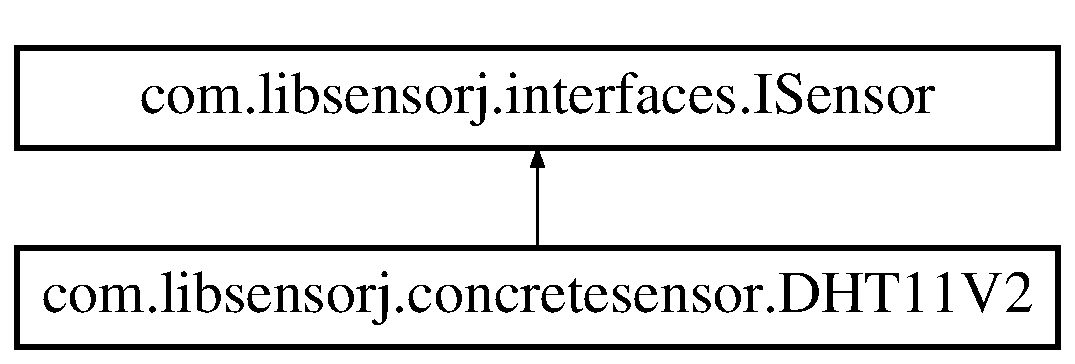
\includegraphics[height=2.000000cm]{classcom_1_1libsensorj_1_1concretesensor_1_1DHT11V2}
\end{center}
\end{figure}
\subsection*{Public Member Functions}
\begin{DoxyCompactItemize}
\item 
\hyperlink{classcom_1_1libsensorj_1_1concretesensor_1_1DHT11V2_a19e1a415c048669c7b4879e02d852682}{D\+H\+T11\+V2} ()
\item 
\hyperlink{classcom_1_1libsensorj_1_1concretesensor_1_1DHT11V2_a2c1a20a2c6796b8dd17629edaa9b4591}{D\+H\+T11\+V2} (int pin)
\item 
\hyperlink{classcom_1_1libsensorj_1_1concretesensor_1_1DHT11V2_a8c3dea8106eef93e12d61f7a7e32e5ca}{D\+H\+T11\+V2} (Pin pin)
\item 
double \hyperlink{classcom_1_1libsensorj_1_1concretesensor_1_1DHT11V2_a883913b8d65fc3e747e22374a8d16bc2}{read\+Value} ()
\item 
synchronized double \hyperlink{classcom_1_1libsensorj_1_1concretesensor_1_1DHT11V2_a3d5619f9ad57662d352dd9ddbf729a23}{get\+Temperature\+In\+Celsius} ()
\item 
synchronized double \hyperlink{classcom_1_1libsensorj_1_1concretesensor_1_1DHT11V2_aa1a825351fad9bd7b0c97abae4a89e05}{get\+Temperature\+In\+Fahrenheit} ()
\item 
synchronized double \hyperlink{classcom_1_1libsensorj_1_1concretesensor_1_1DHT11V2_a86989c9de8a041c8ca9f6f03c0714200}{get\+Temperature\+In\+Kelvin} ()
\item 
void \hyperlink{classcom_1_1libsensorj_1_1concretesensor_1_1DHT11V2_afff27f29285f26230faa8ecda6b6b102}{get\+Instance} ()
\end{DoxyCompactItemize}
\subsection*{Private Member Functions}
\begin{DoxyCompactItemize}
\item 
double \hyperlink{classcom_1_1libsensorj_1_1concretesensor_1_1DHT11V2_a4efa0044c366379af59e24b9570b3ddf}{get\+Temperature} (Temperature\+Scale from)
\item 
boolean \hyperlink{classcom_1_1libsensorj_1_1concretesensor_1_1DHT11V2_a250ebf2e29c3e9c84c840d6f6afc1c00}{check\+Parity} ()
\end{DoxyCompactItemize}
\subsection*{Private Attributes}
\begin{DoxyCompactItemize}
\item 
int\mbox{[}$\,$\mbox{]} \hyperlink{classcom_1_1libsensorj_1_1concretesensor_1_1DHT11V2_a450dd7dfb4fdc23cd25523ad22890ee4}{dht11\+Dat} = \{ 0, 0, 0, 0, 0 \}
\item 
Gpio\+Pin\+Digital\+Multipurpose \hyperlink{classcom_1_1libsensorj_1_1concretesensor_1_1DHT11V2_a04cca3ab141bcf0089fd6a7338a5dabe}{dht11\+Pin}
\end{DoxyCompactItemize}
\subsection*{Static Private Attributes}
\begin{DoxyCompactItemize}
\item 
static final Pin \hyperlink{classcom_1_1libsensorj_1_1concretesensor_1_1DHT11V2_a10e251a19e426166bb913323eee6243b}{D\+E\+F\+A\+U\+L\+T\+\_\+\+P\+I\+N} = Raspi\+Pin.\+G\+P\+I\+O\+\_\+04
\item 
static final int \hyperlink{classcom_1_1libsensorj_1_1concretesensor_1_1DHT11V2_ad64749b474c180fea185aecd512eb656}{M\+A\+X\+T\+I\+M\+I\+N\+G\+S} = 85
\item 
static final Logger \hyperlink{classcom_1_1libsensorj_1_1concretesensor_1_1DHT11V2_acef19b315279adf9b39a4407487d401e}{L\+O\+G\+G\+E\+R}
\end{DoxyCompactItemize}


\subsection{Detailed Description}
The Class \hyperlink{classcom_1_1libsensorj_1_1concretesensor_1_1DHT11V2}{D\+H\+T11\+V2}. 

\subsection{Constructor \& Destructor Documentation}
\hypertarget{classcom_1_1libsensorj_1_1concretesensor_1_1DHT11V2_a19e1a415c048669c7b4879e02d852682}{}\index{com\+::libsensorj\+::concretesensor\+::\+D\+H\+T11\+V2@{com\+::libsensorj\+::concretesensor\+::\+D\+H\+T11\+V2}!D\+H\+T11\+V2@{D\+H\+T11\+V2}}
\index{D\+H\+T11\+V2@{D\+H\+T11\+V2}!com\+::libsensorj\+::concretesensor\+::\+D\+H\+T11\+V2@{com\+::libsensorj\+::concretesensor\+::\+D\+H\+T11\+V2}}
\subsubsection[{D\+H\+T11\+V2}]{\setlength{\rightskip}{0pt plus 5cm}com.\+libsensorj.\+concretesensor.\+D\+H\+T11\+V2.\+D\+H\+T11\+V2 (
\begin{DoxyParamCaption}
{}
\end{DoxyParamCaption}
)}\label{classcom_1_1libsensorj_1_1concretesensor_1_1DHT11V2_a19e1a415c048669c7b4879e02d852682}
Instantiates a new D\+Ht11 v2. \hypertarget{classcom_1_1libsensorj_1_1concretesensor_1_1DHT11V2_a2c1a20a2c6796b8dd17629edaa9b4591}{}\index{com\+::libsensorj\+::concretesensor\+::\+D\+H\+T11\+V2@{com\+::libsensorj\+::concretesensor\+::\+D\+H\+T11\+V2}!D\+H\+T11\+V2@{D\+H\+T11\+V2}}
\index{D\+H\+T11\+V2@{D\+H\+T11\+V2}!com\+::libsensorj\+::concretesensor\+::\+D\+H\+T11\+V2@{com\+::libsensorj\+::concretesensor\+::\+D\+H\+T11\+V2}}
\subsubsection[{D\+H\+T11\+V2}]{\setlength{\rightskip}{0pt plus 5cm}com.\+libsensorj.\+concretesensor.\+D\+H\+T11\+V2.\+D\+H\+T11\+V2 (
\begin{DoxyParamCaption}
\item[{int}]{pin}
\end{DoxyParamCaption}
)}\label{classcom_1_1libsensorj_1_1concretesensor_1_1DHT11V2_a2c1a20a2c6796b8dd17629edaa9b4591}
Instantiates a new D\+Ht11 v2.


\begin{DoxyParams}{Parameters}
{\em pin} & the pin \\
\hline
\end{DoxyParams}
\hypertarget{classcom_1_1libsensorj_1_1concretesensor_1_1DHT11V2_a8c3dea8106eef93e12d61f7a7e32e5ca}{}\index{com\+::libsensorj\+::concretesensor\+::\+D\+H\+T11\+V2@{com\+::libsensorj\+::concretesensor\+::\+D\+H\+T11\+V2}!D\+H\+T11\+V2@{D\+H\+T11\+V2}}
\index{D\+H\+T11\+V2@{D\+H\+T11\+V2}!com\+::libsensorj\+::concretesensor\+::\+D\+H\+T11\+V2@{com\+::libsensorj\+::concretesensor\+::\+D\+H\+T11\+V2}}
\subsubsection[{D\+H\+T11\+V2}]{\setlength{\rightskip}{0pt plus 5cm}com.\+libsensorj.\+concretesensor.\+D\+H\+T11\+V2.\+D\+H\+T11\+V2 (
\begin{DoxyParamCaption}
\item[{Pin}]{pin}
\end{DoxyParamCaption}
)}\label{classcom_1_1libsensorj_1_1concretesensor_1_1DHT11V2_a8c3dea8106eef93e12d61f7a7e32e5ca}
Instantiates a new D\+Ht11 v2.


\begin{DoxyParams}{Parameters}
{\em pin} & the pin \\
\hline
\end{DoxyParams}


\subsection{Member Function Documentation}
\hypertarget{classcom_1_1libsensorj_1_1concretesensor_1_1DHT11V2_a250ebf2e29c3e9c84c840d6f6afc1c00}{}\index{com\+::libsensorj\+::concretesensor\+::\+D\+H\+T11\+V2@{com\+::libsensorj\+::concretesensor\+::\+D\+H\+T11\+V2}!check\+Parity@{check\+Parity}}
\index{check\+Parity@{check\+Parity}!com\+::libsensorj\+::concretesensor\+::\+D\+H\+T11\+V2@{com\+::libsensorj\+::concretesensor\+::\+D\+H\+T11\+V2}}
\subsubsection[{check\+Parity}]{\setlength{\rightskip}{0pt plus 5cm}boolean com.\+libsensorj.\+concretesensor.\+D\+H\+T11\+V2.\+check\+Parity (
\begin{DoxyParamCaption}
{}
\end{DoxyParamCaption}
)\hspace{0.3cm}{\ttfamily [private]}}\label{classcom_1_1libsensorj_1_1concretesensor_1_1DHT11V2_a250ebf2e29c3e9c84c840d6f6afc1c00}
Check parity.

\begin{DoxyReturn}{Returns}
true, if successful 
\end{DoxyReturn}
\hypertarget{classcom_1_1libsensorj_1_1concretesensor_1_1DHT11V2_afff27f29285f26230faa8ecda6b6b102}{}\index{com\+::libsensorj\+::concretesensor\+::\+D\+H\+T11\+V2@{com\+::libsensorj\+::concretesensor\+::\+D\+H\+T11\+V2}!get\+Instance@{get\+Instance}}
\index{get\+Instance@{get\+Instance}!com\+::libsensorj\+::concretesensor\+::\+D\+H\+T11\+V2@{com\+::libsensorj\+::concretesensor\+::\+D\+H\+T11\+V2}}
\subsubsection[{get\+Instance}]{\setlength{\rightskip}{0pt plus 5cm}void com.\+libsensorj.\+concretesensor.\+D\+H\+T11\+V2.\+get\+Instance (
\begin{DoxyParamCaption}
{}
\end{DoxyParamCaption}
)}\label{classcom_1_1libsensorj_1_1concretesensor_1_1DHT11V2_afff27f29285f26230faa8ecda6b6b102}
Gets the single instance of I\+Sensor.

\begin{DoxyReturn}{Returns}
single instance of I\+Sensor 
\end{DoxyReturn}


Implements \hyperlink{interfacecom_1_1libsensorj_1_1interfaces_1_1ISensor_a3c3db93a33adecde81a528651790f75e}{com.\+libsensorj.\+interfaces.\+I\+Sensor}.

\hypertarget{classcom_1_1libsensorj_1_1concretesensor_1_1DHT11V2_a4efa0044c366379af59e24b9570b3ddf}{}\index{com\+::libsensorj\+::concretesensor\+::\+D\+H\+T11\+V2@{com\+::libsensorj\+::concretesensor\+::\+D\+H\+T11\+V2}!get\+Temperature@{get\+Temperature}}
\index{get\+Temperature@{get\+Temperature}!com\+::libsensorj\+::concretesensor\+::\+D\+H\+T11\+V2@{com\+::libsensorj\+::concretesensor\+::\+D\+H\+T11\+V2}}
\subsubsection[{get\+Temperature}]{\setlength{\rightskip}{0pt plus 5cm}double com.\+libsensorj.\+concretesensor.\+D\+H\+T11\+V2.\+get\+Temperature (
\begin{DoxyParamCaption}
\item[{Temperature\+Scale}]{from}
\end{DoxyParamCaption}
)\hspace{0.3cm}{\ttfamily [private]}}\label{classcom_1_1libsensorj_1_1concretesensor_1_1DHT11V2_a4efa0044c366379af59e24b9570b3ddf}
Gets the temperature.


\begin{DoxyParams}{Parameters}
{\em from} & the from \\
\hline
\end{DoxyParams}
\begin{DoxyReturn}{Returns}
the temperature 
\end{DoxyReturn}
\hypertarget{classcom_1_1libsensorj_1_1concretesensor_1_1DHT11V2_a3d5619f9ad57662d352dd9ddbf729a23}{}\index{com\+::libsensorj\+::concretesensor\+::\+D\+H\+T11\+V2@{com\+::libsensorj\+::concretesensor\+::\+D\+H\+T11\+V2}!get\+Temperature\+In\+Celsius@{get\+Temperature\+In\+Celsius}}
\index{get\+Temperature\+In\+Celsius@{get\+Temperature\+In\+Celsius}!com\+::libsensorj\+::concretesensor\+::\+D\+H\+T11\+V2@{com\+::libsensorj\+::concretesensor\+::\+D\+H\+T11\+V2}}
\subsubsection[{get\+Temperature\+In\+Celsius}]{\setlength{\rightskip}{0pt plus 5cm}synchronized double com.\+libsensorj.\+concretesensor.\+D\+H\+T11\+V2.\+get\+Temperature\+In\+Celsius (
\begin{DoxyParamCaption}
{}
\end{DoxyParamCaption}
)}\label{classcom_1_1libsensorj_1_1concretesensor_1_1DHT11V2_a3d5619f9ad57662d352dd9ddbf729a23}
Gets the temperature in celsius.

\begin{DoxyReturn}{Returns}
the temperature in celsius 
\end{DoxyReturn}
\hypertarget{classcom_1_1libsensorj_1_1concretesensor_1_1DHT11V2_aa1a825351fad9bd7b0c97abae4a89e05}{}\index{com\+::libsensorj\+::concretesensor\+::\+D\+H\+T11\+V2@{com\+::libsensorj\+::concretesensor\+::\+D\+H\+T11\+V2}!get\+Temperature\+In\+Fahrenheit@{get\+Temperature\+In\+Fahrenheit}}
\index{get\+Temperature\+In\+Fahrenheit@{get\+Temperature\+In\+Fahrenheit}!com\+::libsensorj\+::concretesensor\+::\+D\+H\+T11\+V2@{com\+::libsensorj\+::concretesensor\+::\+D\+H\+T11\+V2}}
\subsubsection[{get\+Temperature\+In\+Fahrenheit}]{\setlength{\rightskip}{0pt plus 5cm}synchronized double com.\+libsensorj.\+concretesensor.\+D\+H\+T11\+V2.\+get\+Temperature\+In\+Fahrenheit (
\begin{DoxyParamCaption}
{}
\end{DoxyParamCaption}
)}\label{classcom_1_1libsensorj_1_1concretesensor_1_1DHT11V2_aa1a825351fad9bd7b0c97abae4a89e05}
Gets the temperature in fahrenheit.

\begin{DoxyReturn}{Returns}
the temperature in fahrenheit 
\end{DoxyReturn}
\hypertarget{classcom_1_1libsensorj_1_1concretesensor_1_1DHT11V2_a86989c9de8a041c8ca9f6f03c0714200}{}\index{com\+::libsensorj\+::concretesensor\+::\+D\+H\+T11\+V2@{com\+::libsensorj\+::concretesensor\+::\+D\+H\+T11\+V2}!get\+Temperature\+In\+Kelvin@{get\+Temperature\+In\+Kelvin}}
\index{get\+Temperature\+In\+Kelvin@{get\+Temperature\+In\+Kelvin}!com\+::libsensorj\+::concretesensor\+::\+D\+H\+T11\+V2@{com\+::libsensorj\+::concretesensor\+::\+D\+H\+T11\+V2}}
\subsubsection[{get\+Temperature\+In\+Kelvin}]{\setlength{\rightskip}{0pt plus 5cm}synchronized double com.\+libsensorj.\+concretesensor.\+D\+H\+T11\+V2.\+get\+Temperature\+In\+Kelvin (
\begin{DoxyParamCaption}
{}
\end{DoxyParamCaption}
)}\label{classcom_1_1libsensorj_1_1concretesensor_1_1DHT11V2_a86989c9de8a041c8ca9f6f03c0714200}
Gets the temperature in kelvin.

\begin{DoxyReturn}{Returns}
the temperature in kelvin 
\end{DoxyReturn}
\hypertarget{classcom_1_1libsensorj_1_1concretesensor_1_1DHT11V2_a883913b8d65fc3e747e22374a8d16bc2}{}\index{com\+::libsensorj\+::concretesensor\+::\+D\+H\+T11\+V2@{com\+::libsensorj\+::concretesensor\+::\+D\+H\+T11\+V2}!read\+Value@{read\+Value}}
\index{read\+Value@{read\+Value}!com\+::libsensorj\+::concretesensor\+::\+D\+H\+T11\+V2@{com\+::libsensorj\+::concretesensor\+::\+D\+H\+T11\+V2}}
\subsubsection[{read\+Value}]{\setlength{\rightskip}{0pt plus 5cm}double com.\+libsensorj.\+concretesensor.\+D\+H\+T11\+V2.\+read\+Value (
\begin{DoxyParamCaption}
{}
\end{DoxyParamCaption}
)}\label{classcom_1_1libsensorj_1_1concretesensor_1_1DHT11V2_a883913b8d65fc3e747e22374a8d16bc2}
Read value.

\begin{DoxyReturn}{Returns}
the value readed 
\end{DoxyReturn}


\subsection{Member Data Documentation}
\hypertarget{classcom_1_1libsensorj_1_1concretesensor_1_1DHT11V2_a10e251a19e426166bb913323eee6243b}{}\index{com\+::libsensorj\+::concretesensor\+::\+D\+H\+T11\+V2@{com\+::libsensorj\+::concretesensor\+::\+D\+H\+T11\+V2}!D\+E\+F\+A\+U\+L\+T\+\_\+\+P\+I\+N@{D\+E\+F\+A\+U\+L\+T\+\_\+\+P\+I\+N}}
\index{D\+E\+F\+A\+U\+L\+T\+\_\+\+P\+I\+N@{D\+E\+F\+A\+U\+L\+T\+\_\+\+P\+I\+N}!com\+::libsensorj\+::concretesensor\+::\+D\+H\+T11\+V2@{com\+::libsensorj\+::concretesensor\+::\+D\+H\+T11\+V2}}
\subsubsection[{D\+E\+F\+A\+U\+L\+T\+\_\+\+P\+I\+N}]{\setlength{\rightskip}{0pt plus 5cm}final Pin com.\+libsensorj.\+concretesensor.\+D\+H\+T11\+V2.\+D\+E\+F\+A\+U\+L\+T\+\_\+\+P\+I\+N = Raspi\+Pin.\+G\+P\+I\+O\+\_\+04\hspace{0.3cm}{\ttfamily [static]}, {\ttfamily [private]}}\label{classcom_1_1libsensorj_1_1concretesensor_1_1DHT11V2_a10e251a19e426166bb913323eee6243b}
The Constant D\+E\+F\+A\+U\+L\+T\+\_\+\+P\+I\+N. \hypertarget{classcom_1_1libsensorj_1_1concretesensor_1_1DHT11V2_a450dd7dfb4fdc23cd25523ad22890ee4}{}\index{com\+::libsensorj\+::concretesensor\+::\+D\+H\+T11\+V2@{com\+::libsensorj\+::concretesensor\+::\+D\+H\+T11\+V2}!dht11\+Dat@{dht11\+Dat}}
\index{dht11\+Dat@{dht11\+Dat}!com\+::libsensorj\+::concretesensor\+::\+D\+H\+T11\+V2@{com\+::libsensorj\+::concretesensor\+::\+D\+H\+T11\+V2}}
\subsubsection[{dht11\+Dat}]{\setlength{\rightskip}{0pt plus 5cm}int \mbox{[}$\,$\mbox{]} com.\+libsensorj.\+concretesensor.\+D\+H\+T11\+V2.\+dht11\+Dat = \{ 0, 0, 0, 0, 0 \}\hspace{0.3cm}{\ttfamily [private]}}\label{classcom_1_1libsensorj_1_1concretesensor_1_1DHT11V2_a450dd7dfb4fdc23cd25523ad22890ee4}
The dht11\+Dat. \hypertarget{classcom_1_1libsensorj_1_1concretesensor_1_1DHT11V2_a04cca3ab141bcf0089fd6a7338a5dabe}{}\index{com\+::libsensorj\+::concretesensor\+::\+D\+H\+T11\+V2@{com\+::libsensorj\+::concretesensor\+::\+D\+H\+T11\+V2}!dht11\+Pin@{dht11\+Pin}}
\index{dht11\+Pin@{dht11\+Pin}!com\+::libsensorj\+::concretesensor\+::\+D\+H\+T11\+V2@{com\+::libsensorj\+::concretesensor\+::\+D\+H\+T11\+V2}}
\subsubsection[{dht11\+Pin}]{\setlength{\rightskip}{0pt plus 5cm}Gpio\+Pin\+Digital\+Multipurpose com.\+libsensorj.\+concretesensor.\+D\+H\+T11\+V2.\+dht11\+Pin\hspace{0.3cm}{\ttfamily [private]}}\label{classcom_1_1libsensorj_1_1concretesensor_1_1DHT11V2_a04cca3ab141bcf0089fd6a7338a5dabe}
The dht11 pin. \hypertarget{classcom_1_1libsensorj_1_1concretesensor_1_1DHT11V2_acef19b315279adf9b39a4407487d401e}{}\index{com\+::libsensorj\+::concretesensor\+::\+D\+H\+T11\+V2@{com\+::libsensorj\+::concretesensor\+::\+D\+H\+T11\+V2}!L\+O\+G\+G\+E\+R@{L\+O\+G\+G\+E\+R}}
\index{L\+O\+G\+G\+E\+R@{L\+O\+G\+G\+E\+R}!com\+::libsensorj\+::concretesensor\+::\+D\+H\+T11\+V2@{com\+::libsensorj\+::concretesensor\+::\+D\+H\+T11\+V2}}
\subsubsection[{L\+O\+G\+G\+E\+R}]{\setlength{\rightskip}{0pt plus 5cm}final Logger com.\+libsensorj.\+concretesensor.\+D\+H\+T11\+V2.\+L\+O\+G\+G\+E\+R\hspace{0.3cm}{\ttfamily [static]}, {\ttfamily [private]}}\label{classcom_1_1libsensorj_1_1concretesensor_1_1DHT11V2_acef19b315279adf9b39a4407487d401e}
{\bfseries Initial value\+:}
\begin{DoxyCode}
= LogManager.getLogger(\hyperlink{classcom_1_1libsensorj_1_1concretesensor_1_1DHT11V2_a19e1a415c048669c7b4879e02d852682}{DHT11V2}.class
            .getName())
\end{DoxyCode}
The Constant L\+O\+G\+G\+E\+R. \hypertarget{classcom_1_1libsensorj_1_1concretesensor_1_1DHT11V2_ad64749b474c180fea185aecd512eb656}{}\index{com\+::libsensorj\+::concretesensor\+::\+D\+H\+T11\+V2@{com\+::libsensorj\+::concretesensor\+::\+D\+H\+T11\+V2}!M\+A\+X\+T\+I\+M\+I\+N\+G\+S@{M\+A\+X\+T\+I\+M\+I\+N\+G\+S}}
\index{M\+A\+X\+T\+I\+M\+I\+N\+G\+S@{M\+A\+X\+T\+I\+M\+I\+N\+G\+S}!com\+::libsensorj\+::concretesensor\+::\+D\+H\+T11\+V2@{com\+::libsensorj\+::concretesensor\+::\+D\+H\+T11\+V2}}
\subsubsection[{M\+A\+X\+T\+I\+M\+I\+N\+G\+S}]{\setlength{\rightskip}{0pt plus 5cm}final int com.\+libsensorj.\+concretesensor.\+D\+H\+T11\+V2.\+M\+A\+X\+T\+I\+M\+I\+N\+G\+S = 85\hspace{0.3cm}{\ttfamily [static]}, {\ttfamily [private]}}\label{classcom_1_1libsensorj_1_1concretesensor_1_1DHT11V2_ad64749b474c180fea185aecd512eb656}
The Constant M\+A\+X\+T\+I\+M\+I\+N\+G\+S. 

The documentation for this class was generated from the following file\+:\begin{DoxyCompactItemize}
\item 
main/java/com/libsensorj/concretesensor/\hyperlink{DHT11V2_8java}{D\+H\+T11\+V2.\+java}\end{DoxyCompactItemize}

\hypertarget{classcom_1_1libsensorj_1_1examples_1_1DHT11V2Example}{}\section{com.\+libsensorj.\+examples.\+D\+H\+T11\+V2\+Example Class Reference}
\label{classcom_1_1libsensorj_1_1examples_1_1DHT11V2Example}\index{com.\+libsensorj.\+examples.\+D\+H\+T11\+V2\+Example@{com.\+libsensorj.\+examples.\+D\+H\+T11\+V2\+Example}}
\subsection*{Static Public Member Functions}
\begin{DoxyCompactItemize}
\item 
static void \hyperlink{classcom_1_1libsensorj_1_1examples_1_1DHT11V2Example_a423db1184c15475e4b120b7f2783545b}{main} (String\mbox{[}$\,$\mbox{]} args)
\end{DoxyCompactItemize}
\subsection*{Static Private Attributes}
\begin{DoxyCompactItemize}
\item 
static \hyperlink{interfacecom_1_1libsensorj_1_1interfaces_1_1ISensor}{I\+Sensor} \hyperlink{classcom_1_1libsensorj_1_1examples_1_1DHT11V2Example_a5bc507916742167876ff258c298163ed}{dht11}
\item 
static final Logger \hyperlink{classcom_1_1libsensorj_1_1examples_1_1DHT11V2Example_a962cfebacb8855647655c3b6c0f6f698}{L\+O\+G\+G\+E\+R}
\end{DoxyCompactItemize}


\subsection{Detailed Description}
The Class \hyperlink{classcom_1_1libsensorj_1_1examples_1_1DHT11V2Example}{D\+H\+T11\+V2\+Example}. 

\subsection{Member Function Documentation}
\hypertarget{classcom_1_1libsensorj_1_1examples_1_1DHT11V2Example_a423db1184c15475e4b120b7f2783545b}{}\index{com\+::libsensorj\+::examples\+::\+D\+H\+T11\+V2\+Example@{com\+::libsensorj\+::examples\+::\+D\+H\+T11\+V2\+Example}!main@{main}}
\index{main@{main}!com\+::libsensorj\+::examples\+::\+D\+H\+T11\+V2\+Example@{com\+::libsensorj\+::examples\+::\+D\+H\+T11\+V2\+Example}}
\subsubsection[{main}]{\setlength{\rightskip}{0pt plus 5cm}static void com.\+libsensorj.\+examples.\+D\+H\+T11\+V2\+Example.\+main (
\begin{DoxyParamCaption}
\item[{String\mbox{[}$\,$\mbox{]}}]{args}
\end{DoxyParamCaption}
)\hspace{0.3cm}{\ttfamily [static]}}\label{classcom_1_1libsensorj_1_1examples_1_1DHT11V2Example_a423db1184c15475e4b120b7f2783545b}
The main method.


\begin{DoxyParams}{Parameters}
{\em args} & the arguments \\
\hline
\end{DoxyParams}


\subsection{Member Data Documentation}
\hypertarget{classcom_1_1libsensorj_1_1examples_1_1DHT11V2Example_a5bc507916742167876ff258c298163ed}{}\index{com\+::libsensorj\+::examples\+::\+D\+H\+T11\+V2\+Example@{com\+::libsensorj\+::examples\+::\+D\+H\+T11\+V2\+Example}!dht11@{dht11}}
\index{dht11@{dht11}!com\+::libsensorj\+::examples\+::\+D\+H\+T11\+V2\+Example@{com\+::libsensorj\+::examples\+::\+D\+H\+T11\+V2\+Example}}
\subsubsection[{dht11}]{\setlength{\rightskip}{0pt plus 5cm}{\bf I\+Sensor} com.\+libsensorj.\+examples.\+D\+H\+T11\+V2\+Example.\+dht11\hspace{0.3cm}{\ttfamily [static]}, {\ttfamily [private]}}\label{classcom_1_1libsensorj_1_1examples_1_1DHT11V2Example_a5bc507916742167876ff258c298163ed}
The I\+Sensor dht11. \hypertarget{classcom_1_1libsensorj_1_1examples_1_1DHT11V2Example_a962cfebacb8855647655c3b6c0f6f698}{}\index{com\+::libsensorj\+::examples\+::\+D\+H\+T11\+V2\+Example@{com\+::libsensorj\+::examples\+::\+D\+H\+T11\+V2\+Example}!L\+O\+G\+G\+E\+R@{L\+O\+G\+G\+E\+R}}
\index{L\+O\+G\+G\+E\+R@{L\+O\+G\+G\+E\+R}!com\+::libsensorj\+::examples\+::\+D\+H\+T11\+V2\+Example@{com\+::libsensorj\+::examples\+::\+D\+H\+T11\+V2\+Example}}
\subsubsection[{L\+O\+G\+G\+E\+R}]{\setlength{\rightskip}{0pt plus 5cm}final Logger com.\+libsensorj.\+examples.\+D\+H\+T11\+V2\+Example.\+L\+O\+G\+G\+E\+R\hspace{0.3cm}{\ttfamily [static]}, {\ttfamily [private]}}\label{classcom_1_1libsensorj_1_1examples_1_1DHT11V2Example_a962cfebacb8855647655c3b6c0f6f698}
{\bfseries Initial value\+:}
\begin{DoxyCode}
= LogManager
            .getLogger(DHT11TemperatureExample.class.getName())
\end{DoxyCode}
The Constant L\+O\+G\+G\+E\+R. 

The documentation for this class was generated from the following file\+:\begin{DoxyCompactItemize}
\item 
main/java/com/libsensorj/examples/\hyperlink{DHT11V2Example_8java}{D\+H\+T11\+V2\+Example.\+java}\end{DoxyCompactItemize}

\hypertarget{classcom_1_1libsensorj_1_1concretefactory_1_1DHT11V2Factory}{}\section{com.\+libsensorj.\+concretefactory.\+D\+H\+T11\+V2\+Factory Class Reference}
\label{classcom_1_1libsensorj_1_1concretefactory_1_1DHT11V2Factory}\index{com.\+libsensorj.\+concretefactory.\+D\+H\+T11\+V2\+Factory@{com.\+libsensorj.\+concretefactory.\+D\+H\+T11\+V2\+Factory}}
Inheritance diagram for com.\+libsensorj.\+concretefactory.\+D\+H\+T11\+V2\+Factory\+:\begin{figure}[H]
\begin{center}
\leavevmode
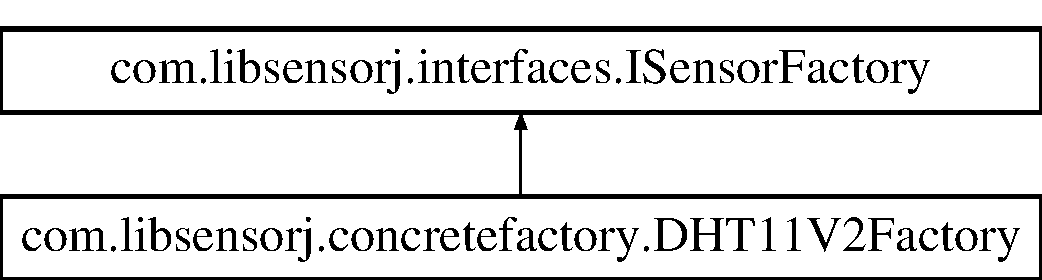
\includegraphics[height=2.000000cm]{classcom_1_1libsensorj_1_1concretefactory_1_1DHT11V2Factory}
\end{center}
\end{figure}
\subsection*{Public Member Functions}
\begin{DoxyCompactItemize}
\item 
\hyperlink{interfacecom_1_1libsensorj_1_1interfaces_1_1ISensor}{I\+Sensor} \hyperlink{classcom_1_1libsensorj_1_1concretefactory_1_1DHT11V2Factory_ac04eaebc748d420eb035439dfc1d2202}{create\+Sensor} ()
\item 
\hyperlink{classcom_1_1libsensorj_1_1interfaces_1_1IEvent}{I\+Event} \hyperlink{classcom_1_1libsensorj_1_1concretefactory_1_1DHT11V2Factory_a0eb0b480f4133c3eeb2728bd0fa45c58}{create\+Event} ()
\item 
synchronized double \hyperlink{classcom_1_1libsensorj_1_1concretefactory_1_1DHT11V2Factory_a2c966faecd375072c885ca7dadb76530}{get\+Temperature\+In\+Celsius} ()
\item 
synchronized double \hyperlink{classcom_1_1libsensorj_1_1concretefactory_1_1DHT11V2Factory_a1716289d2f7d918b7daa8b61fece0712}{get\+Temperature\+In\+Fahrenheit} ()
\item 
synchronized double \hyperlink{classcom_1_1libsensorj_1_1concretefactory_1_1DHT11V2Factory_a9524a22ee17f7382aa40bd9350ddc21f}{get\+Temperature\+In\+Kelvin} ()
\end{DoxyCompactItemize}
\subsection*{Static Public Member Functions}
\begin{DoxyCompactItemize}
\item 
static \hyperlink{classcom_1_1libsensorj_1_1concretesensor_1_1DHT11V2}{D\+H\+T11\+V2} \hyperlink{classcom_1_1libsensorj_1_1concretefactory_1_1DHT11V2Factory_abf6c846a1ccc76d082cee9215df1596c}{get\+Instance} ()
\end{DoxyCompactItemize}
\subsection*{Private Member Functions}
\begin{DoxyCompactItemize}
\item 
\hyperlink{classcom_1_1libsensorj_1_1concretefactory_1_1DHT11V2Factory_a6daec5c65e3b39f2e4770a583271a107}{D\+H\+T11\+V2\+Factory} ()
\end{DoxyCompactItemize}
\subsection*{Static Private Attributes}
\begin{DoxyCompactItemize}
\item 
static \hyperlink{classcom_1_1libsensorj_1_1concretesensor_1_1DHT11V2}{D\+H\+T11\+V2} \hyperlink{classcom_1_1libsensorj_1_1concretefactory_1_1DHT11V2Factory_a9ec0e463b94ba2654e29ab495805deeb}{dht11}
\end{DoxyCompactItemize}


\subsection{Detailed Description}
A factory for creating D\+H\+T11\+V2 objects. 

\subsection{Constructor \& Destructor Documentation}
\hypertarget{classcom_1_1libsensorj_1_1concretefactory_1_1DHT11V2Factory_a6daec5c65e3b39f2e4770a583271a107}{}\index{com\+::libsensorj\+::concretefactory\+::\+D\+H\+T11\+V2\+Factory@{com\+::libsensorj\+::concretefactory\+::\+D\+H\+T11\+V2\+Factory}!D\+H\+T11\+V2\+Factory@{D\+H\+T11\+V2\+Factory}}
\index{D\+H\+T11\+V2\+Factory@{D\+H\+T11\+V2\+Factory}!com\+::libsensorj\+::concretefactory\+::\+D\+H\+T11\+V2\+Factory@{com\+::libsensorj\+::concretefactory\+::\+D\+H\+T11\+V2\+Factory}}
\subsubsection[{D\+H\+T11\+V2\+Factory}]{\setlength{\rightskip}{0pt plus 5cm}com.\+libsensorj.\+concretefactory.\+D\+H\+T11\+V2\+Factory.\+D\+H\+T11\+V2\+Factory (
\begin{DoxyParamCaption}
{}
\end{DoxyParamCaption}
)\hspace{0.3cm}{\ttfamily [private]}}\label{classcom_1_1libsensorj_1_1concretefactory_1_1DHT11V2Factory_a6daec5c65e3b39f2e4770a583271a107}
Instantiates a new D\+Ht11 v2 factory. 

\subsection{Member Function Documentation}
\hypertarget{classcom_1_1libsensorj_1_1concretefactory_1_1DHT11V2Factory_a0eb0b480f4133c3eeb2728bd0fa45c58}{}\index{com\+::libsensorj\+::concretefactory\+::\+D\+H\+T11\+V2\+Factory@{com\+::libsensorj\+::concretefactory\+::\+D\+H\+T11\+V2\+Factory}!create\+Event@{create\+Event}}
\index{create\+Event@{create\+Event}!com\+::libsensorj\+::concretefactory\+::\+D\+H\+T11\+V2\+Factory@{com\+::libsensorj\+::concretefactory\+::\+D\+H\+T11\+V2\+Factory}}
\subsubsection[{create\+Event}]{\setlength{\rightskip}{0pt plus 5cm}{\bf I\+Event} com.\+libsensorj.\+concretefactory.\+D\+H\+T11\+V2\+Factory.\+create\+Event (
\begin{DoxyParamCaption}
{}
\end{DoxyParamCaption}
)}\label{classcom_1_1libsensorj_1_1concretefactory_1_1DHT11V2Factory_a0eb0b480f4133c3eeb2728bd0fa45c58}
Creates a new I\+Event object.

\begin{DoxyReturn}{Returns}
the I\+Event 
\end{DoxyReturn}


Implements \hyperlink{interfacecom_1_1libsensorj_1_1interfaces_1_1ISensorFactory_a2b074d01287a4e64677097255ba9e768}{com.\+libsensorj.\+interfaces.\+I\+Sensor\+Factory}.

\hypertarget{classcom_1_1libsensorj_1_1concretefactory_1_1DHT11V2Factory_ac04eaebc748d420eb035439dfc1d2202}{}\index{com\+::libsensorj\+::concretefactory\+::\+D\+H\+T11\+V2\+Factory@{com\+::libsensorj\+::concretefactory\+::\+D\+H\+T11\+V2\+Factory}!create\+Sensor@{create\+Sensor}}
\index{create\+Sensor@{create\+Sensor}!com\+::libsensorj\+::concretefactory\+::\+D\+H\+T11\+V2\+Factory@{com\+::libsensorj\+::concretefactory\+::\+D\+H\+T11\+V2\+Factory}}
\subsubsection[{create\+Sensor}]{\setlength{\rightskip}{0pt plus 5cm}{\bf I\+Sensor} com.\+libsensorj.\+concretefactory.\+D\+H\+T11\+V2\+Factory.\+create\+Sensor (
\begin{DoxyParamCaption}
{}
\end{DoxyParamCaption}
)}\label{classcom_1_1libsensorj_1_1concretefactory_1_1DHT11V2Factory_ac04eaebc748d420eb035439dfc1d2202}
Creates a new I\+Sensor object.

\begin{DoxyReturn}{Returns}
the I\+Sensor 
\end{DoxyReturn}


Implements \hyperlink{interfacecom_1_1libsensorj_1_1interfaces_1_1ISensorFactory_ac14c6d566c37c6a79c6db1e85634f25d}{com.\+libsensorj.\+interfaces.\+I\+Sensor\+Factory}.

\hypertarget{classcom_1_1libsensorj_1_1concretefactory_1_1DHT11V2Factory_abf6c846a1ccc76d082cee9215df1596c}{}\index{com\+::libsensorj\+::concretefactory\+::\+D\+H\+T11\+V2\+Factory@{com\+::libsensorj\+::concretefactory\+::\+D\+H\+T11\+V2\+Factory}!get\+Instance@{get\+Instance}}
\index{get\+Instance@{get\+Instance}!com\+::libsensorj\+::concretefactory\+::\+D\+H\+T11\+V2\+Factory@{com\+::libsensorj\+::concretefactory\+::\+D\+H\+T11\+V2\+Factory}}
\subsubsection[{get\+Instance}]{\setlength{\rightskip}{0pt plus 5cm}static {\bf D\+H\+T11\+V2} com.\+libsensorj.\+concretefactory.\+D\+H\+T11\+V2\+Factory.\+get\+Instance (
\begin{DoxyParamCaption}
{}
\end{DoxyParamCaption}
)\hspace{0.3cm}{\ttfamily [static]}}\label{classcom_1_1libsensorj_1_1concretefactory_1_1DHT11V2Factory_abf6c846a1ccc76d082cee9215df1596c}
Gets the single instance of \hyperlink{classcom_1_1libsensorj_1_1concretefactory_1_1DHT11V2Factory}{D\+H\+T11\+V2\+Factory}.

\begin{DoxyReturn}{Returns}
single instance of \hyperlink{classcom_1_1libsensorj_1_1concretefactory_1_1DHT11V2Factory}{D\+H\+T11\+V2\+Factory} 
\end{DoxyReturn}
\hypertarget{classcom_1_1libsensorj_1_1concretefactory_1_1DHT11V2Factory_a2c966faecd375072c885ca7dadb76530}{}\index{com\+::libsensorj\+::concretefactory\+::\+D\+H\+T11\+V2\+Factory@{com\+::libsensorj\+::concretefactory\+::\+D\+H\+T11\+V2\+Factory}!get\+Temperature\+In\+Celsius@{get\+Temperature\+In\+Celsius}}
\index{get\+Temperature\+In\+Celsius@{get\+Temperature\+In\+Celsius}!com\+::libsensorj\+::concretefactory\+::\+D\+H\+T11\+V2\+Factory@{com\+::libsensorj\+::concretefactory\+::\+D\+H\+T11\+V2\+Factory}}
\subsubsection[{get\+Temperature\+In\+Celsius}]{\setlength{\rightskip}{0pt plus 5cm}synchronized double com.\+libsensorj.\+concretefactory.\+D\+H\+T11\+V2\+Factory.\+get\+Temperature\+In\+Celsius (
\begin{DoxyParamCaption}
{}
\end{DoxyParamCaption}
)}\label{classcom_1_1libsensorj_1_1concretefactory_1_1DHT11V2Factory_a2c966faecd375072c885ca7dadb76530}
Gets the temperature in celsius.

\begin{DoxyReturn}{Returns}
the temperature in celsius 
\end{DoxyReturn}
\hypertarget{classcom_1_1libsensorj_1_1concretefactory_1_1DHT11V2Factory_a1716289d2f7d918b7daa8b61fece0712}{}\index{com\+::libsensorj\+::concretefactory\+::\+D\+H\+T11\+V2\+Factory@{com\+::libsensorj\+::concretefactory\+::\+D\+H\+T11\+V2\+Factory}!get\+Temperature\+In\+Fahrenheit@{get\+Temperature\+In\+Fahrenheit}}
\index{get\+Temperature\+In\+Fahrenheit@{get\+Temperature\+In\+Fahrenheit}!com\+::libsensorj\+::concretefactory\+::\+D\+H\+T11\+V2\+Factory@{com\+::libsensorj\+::concretefactory\+::\+D\+H\+T11\+V2\+Factory}}
\subsubsection[{get\+Temperature\+In\+Fahrenheit}]{\setlength{\rightskip}{0pt plus 5cm}synchronized double com.\+libsensorj.\+concretefactory.\+D\+H\+T11\+V2\+Factory.\+get\+Temperature\+In\+Fahrenheit (
\begin{DoxyParamCaption}
{}
\end{DoxyParamCaption}
)}\label{classcom_1_1libsensorj_1_1concretefactory_1_1DHT11V2Factory_a1716289d2f7d918b7daa8b61fece0712}
Gets the temperature in fahrenheit.

\begin{DoxyReturn}{Returns}
the temperature in fahrenheit 
\end{DoxyReturn}
\hypertarget{classcom_1_1libsensorj_1_1concretefactory_1_1DHT11V2Factory_a9524a22ee17f7382aa40bd9350ddc21f}{}\index{com\+::libsensorj\+::concretefactory\+::\+D\+H\+T11\+V2\+Factory@{com\+::libsensorj\+::concretefactory\+::\+D\+H\+T11\+V2\+Factory}!get\+Temperature\+In\+Kelvin@{get\+Temperature\+In\+Kelvin}}
\index{get\+Temperature\+In\+Kelvin@{get\+Temperature\+In\+Kelvin}!com\+::libsensorj\+::concretefactory\+::\+D\+H\+T11\+V2\+Factory@{com\+::libsensorj\+::concretefactory\+::\+D\+H\+T11\+V2\+Factory}}
\subsubsection[{get\+Temperature\+In\+Kelvin}]{\setlength{\rightskip}{0pt plus 5cm}synchronized double com.\+libsensorj.\+concretefactory.\+D\+H\+T11\+V2\+Factory.\+get\+Temperature\+In\+Kelvin (
\begin{DoxyParamCaption}
{}
\end{DoxyParamCaption}
)}\label{classcom_1_1libsensorj_1_1concretefactory_1_1DHT11V2Factory_a9524a22ee17f7382aa40bd9350ddc21f}
Gets the temperature in kelvin.

\begin{DoxyReturn}{Returns}
the temperature in kelvin 
\end{DoxyReturn}


\subsection{Member Data Documentation}
\hypertarget{classcom_1_1libsensorj_1_1concretefactory_1_1DHT11V2Factory_a9ec0e463b94ba2654e29ab495805deeb}{}\index{com\+::libsensorj\+::concretefactory\+::\+D\+H\+T11\+V2\+Factory@{com\+::libsensorj\+::concretefactory\+::\+D\+H\+T11\+V2\+Factory}!dht11@{dht11}}
\index{dht11@{dht11}!com\+::libsensorj\+::concretefactory\+::\+D\+H\+T11\+V2\+Factory@{com\+::libsensorj\+::concretefactory\+::\+D\+H\+T11\+V2\+Factory}}
\subsubsection[{dht11}]{\setlength{\rightskip}{0pt plus 5cm}{\bf D\+H\+T11\+V2} com.\+libsensorj.\+concretefactory.\+D\+H\+T11\+V2\+Factory.\+dht11\hspace{0.3cm}{\ttfamily [static]}, {\ttfamily [private]}}\label{classcom_1_1libsensorj_1_1concretefactory_1_1DHT11V2Factory_a9ec0e463b94ba2654e29ab495805deeb}
The dht11. 

The documentation for this class was generated from the following file\+:\begin{DoxyCompactItemize}
\item 
main/java/com/libsensorj/concretefactory/\hyperlink{DHT11V2Factory_8java}{D\+H\+T11\+V2\+Factory.\+java}\end{DoxyCompactItemize}

\hypertarget{classcom_1_1libsensorj_1_1concretesensor_1_1DHT11V3}{}\section{com.\+libsensorj.\+concretesensor.\+D\+H\+T11\+V3 Class Reference}
\label{classcom_1_1libsensorj_1_1concretesensor_1_1DHT11V3}\index{com.\+libsensorj.\+concretesensor.\+D\+H\+T11\+V3@{com.\+libsensorj.\+concretesensor.\+D\+H\+T11\+V3}}
Inheritance diagram for com.\+libsensorj.\+concretesensor.\+D\+H\+T11\+V3\+:\begin{figure}[H]
\begin{center}
\leavevmode
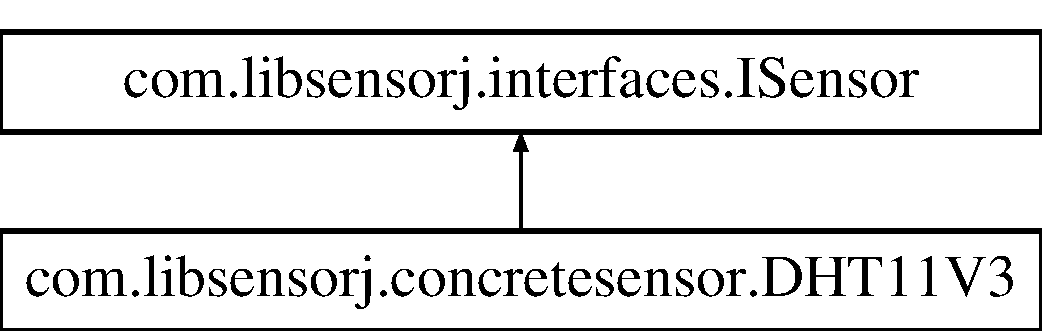
\includegraphics[height=2.000000cm]{classcom_1_1libsensorj_1_1concretesensor_1_1DHT11V3}
\end{center}
\end{figure}
\subsection*{Public Member Functions}
\begin{DoxyCompactItemize}
\item 
\hyperlink{classcom_1_1libsensorj_1_1concretesensor_1_1DHT11V3_a4996e16bdabeb71e35d8358a7e8248ca}{D\+H\+T11\+V3} ()
\item 
\hyperlink{classcom_1_1libsensorj_1_1concretesensor_1_1DHT11V3_a996dadcfe1bd20cd07d94be5c31b5453}{D\+H\+T11\+V3} (int pin)
\item 
\hyperlink{classcom_1_1libsensorj_1_1concretesensor_1_1DHT11V3_a1b40e6e4ec8ddd4df32c86d2dbe280b4}{D\+H\+T11\+V3} (Pin pin)
\item 
double \hyperlink{classcom_1_1libsensorj_1_1concretesensor_1_1DHT11V3_a15f5982dba996cc76bb7d0722ed70d31}{read\+Value} ()
\item 
synchronized double \hyperlink{classcom_1_1libsensorj_1_1concretesensor_1_1DHT11V3_afb1b93f01e2d40f12d9889217e5a37ee}{get\+Temperature\+In\+Celsius} ()
\item 
synchronized double \hyperlink{classcom_1_1libsensorj_1_1concretesensor_1_1DHT11V3_a7d1e369f920792870655add65dfed553}{get\+Temperature\+In\+Fahrenheit} ()
\item 
synchronized double \hyperlink{classcom_1_1libsensorj_1_1concretesensor_1_1DHT11V3_a3c8ecacf36b2b4d2de219dd9912b64b5}{get\+Temperature\+In\+Kelvin} ()
\item 
void \hyperlink{classcom_1_1libsensorj_1_1concretesensor_1_1DHT11V3_a94e402a3ea89ad3ee46725fdd64b4c82}{get\+Instance} ()
\end{DoxyCompactItemize}
\subsection*{Private Member Functions}
\begin{DoxyCompactItemize}
\item 
double \hyperlink{classcom_1_1libsensorj_1_1concretesensor_1_1DHT11V3_aba55ef9b04ccfa46d57079a526da9082}{get\+Temperature} (Temperature\+Scale from)
\end{DoxyCompactItemize}
\subsection*{Private Attributes}
\begin{DoxyCompactItemize}
\item 
int \hyperlink{classcom_1_1libsensorj_1_1concretesensor_1_1DHT11V3_a0c34b9cc559817c10910b1a6180decfd}{temperature}
\item 
Gpio\+Pin\+Digital\+Multipurpose \hyperlink{classcom_1_1libsensorj_1_1concretesensor_1_1DHT11V3_ab72b7b7ed1bd497e7b2818147afeeba9}{dht11\+Pin}
\end{DoxyCompactItemize}
\subsection*{Static Private Attributes}
\begin{DoxyCompactItemize}
\item 
static final Pin \hyperlink{classcom_1_1libsensorj_1_1concretesensor_1_1DHT11V3_a5abd2ea6b296cbd458df3e9170201913}{D\+E\+F\+A\+U\+L\+T\+\_\+\+P\+I\+N} = Raspi\+Pin.\+G\+P\+I\+O\+\_\+04
\item 
static final Logger \hyperlink{classcom_1_1libsensorj_1_1concretesensor_1_1DHT11V3_ac0cd3bfc7916b033ac50cebead5ba268}{L\+O\+G\+G\+E\+R}
\end{DoxyCompactItemize}


\subsection{Detailed Description}
The Class \hyperlink{classcom_1_1libsensorj_1_1concretesensor_1_1DHT11V3}{D\+H\+T11\+V3}. 

\subsection{Constructor \& Destructor Documentation}
\hypertarget{classcom_1_1libsensorj_1_1concretesensor_1_1DHT11V3_a4996e16bdabeb71e35d8358a7e8248ca}{}\index{com\+::libsensorj\+::concretesensor\+::\+D\+H\+T11\+V3@{com\+::libsensorj\+::concretesensor\+::\+D\+H\+T11\+V3}!D\+H\+T11\+V3@{D\+H\+T11\+V3}}
\index{D\+H\+T11\+V3@{D\+H\+T11\+V3}!com\+::libsensorj\+::concretesensor\+::\+D\+H\+T11\+V3@{com\+::libsensorj\+::concretesensor\+::\+D\+H\+T11\+V3}}
\subsubsection[{D\+H\+T11\+V3}]{\setlength{\rightskip}{0pt plus 5cm}com.\+libsensorj.\+concretesensor.\+D\+H\+T11\+V3.\+D\+H\+T11\+V3 (
\begin{DoxyParamCaption}
{}
\end{DoxyParamCaption}
)}\label{classcom_1_1libsensorj_1_1concretesensor_1_1DHT11V3_a4996e16bdabeb71e35d8358a7e8248ca}
Instantiates a new D\+Ht11 v3. \hypertarget{classcom_1_1libsensorj_1_1concretesensor_1_1DHT11V3_a996dadcfe1bd20cd07d94be5c31b5453}{}\index{com\+::libsensorj\+::concretesensor\+::\+D\+H\+T11\+V3@{com\+::libsensorj\+::concretesensor\+::\+D\+H\+T11\+V3}!D\+H\+T11\+V3@{D\+H\+T11\+V3}}
\index{D\+H\+T11\+V3@{D\+H\+T11\+V3}!com\+::libsensorj\+::concretesensor\+::\+D\+H\+T11\+V3@{com\+::libsensorj\+::concretesensor\+::\+D\+H\+T11\+V3}}
\subsubsection[{D\+H\+T11\+V3}]{\setlength{\rightskip}{0pt plus 5cm}com.\+libsensorj.\+concretesensor.\+D\+H\+T11\+V3.\+D\+H\+T11\+V3 (
\begin{DoxyParamCaption}
\item[{int}]{pin}
\end{DoxyParamCaption}
)}\label{classcom_1_1libsensorj_1_1concretesensor_1_1DHT11V3_a996dadcfe1bd20cd07d94be5c31b5453}
Instantiates a new D\+Ht11 v3.


\begin{DoxyParams}{Parameters}
{\em pin} & the pin \\
\hline
\end{DoxyParams}
\hypertarget{classcom_1_1libsensorj_1_1concretesensor_1_1DHT11V3_a1b40e6e4ec8ddd4df32c86d2dbe280b4}{}\index{com\+::libsensorj\+::concretesensor\+::\+D\+H\+T11\+V3@{com\+::libsensorj\+::concretesensor\+::\+D\+H\+T11\+V3}!D\+H\+T11\+V3@{D\+H\+T11\+V3}}
\index{D\+H\+T11\+V3@{D\+H\+T11\+V3}!com\+::libsensorj\+::concretesensor\+::\+D\+H\+T11\+V3@{com\+::libsensorj\+::concretesensor\+::\+D\+H\+T11\+V3}}
\subsubsection[{D\+H\+T11\+V3}]{\setlength{\rightskip}{0pt plus 5cm}com.\+libsensorj.\+concretesensor.\+D\+H\+T11\+V3.\+D\+H\+T11\+V3 (
\begin{DoxyParamCaption}
\item[{Pin}]{pin}
\end{DoxyParamCaption}
)}\label{classcom_1_1libsensorj_1_1concretesensor_1_1DHT11V3_a1b40e6e4ec8ddd4df32c86d2dbe280b4}
Instantiates a new D\+Ht11 v3.


\begin{DoxyParams}{Parameters}
{\em pin} & the pin \\
\hline
\end{DoxyParams}


\subsection{Member Function Documentation}
\hypertarget{classcom_1_1libsensorj_1_1concretesensor_1_1DHT11V3_a94e402a3ea89ad3ee46725fdd64b4c82}{}\index{com\+::libsensorj\+::concretesensor\+::\+D\+H\+T11\+V3@{com\+::libsensorj\+::concretesensor\+::\+D\+H\+T11\+V3}!get\+Instance@{get\+Instance}}
\index{get\+Instance@{get\+Instance}!com\+::libsensorj\+::concretesensor\+::\+D\+H\+T11\+V3@{com\+::libsensorj\+::concretesensor\+::\+D\+H\+T11\+V3}}
\subsubsection[{get\+Instance}]{\setlength{\rightskip}{0pt plus 5cm}void com.\+libsensorj.\+concretesensor.\+D\+H\+T11\+V3.\+get\+Instance (
\begin{DoxyParamCaption}
{}
\end{DoxyParamCaption}
)}\label{classcom_1_1libsensorj_1_1concretesensor_1_1DHT11V3_a94e402a3ea89ad3ee46725fdd64b4c82}
Gets the single instance of I\+Sensor.

\begin{DoxyReturn}{Returns}
single instance of I\+Sensor 
\end{DoxyReturn}


Implements \hyperlink{interfacecom_1_1libsensorj_1_1interfaces_1_1ISensor_a3c3db93a33adecde81a528651790f75e}{com.\+libsensorj.\+interfaces.\+I\+Sensor}.

\hypertarget{classcom_1_1libsensorj_1_1concretesensor_1_1DHT11V3_aba55ef9b04ccfa46d57079a526da9082}{}\index{com\+::libsensorj\+::concretesensor\+::\+D\+H\+T11\+V3@{com\+::libsensorj\+::concretesensor\+::\+D\+H\+T11\+V3}!get\+Temperature@{get\+Temperature}}
\index{get\+Temperature@{get\+Temperature}!com\+::libsensorj\+::concretesensor\+::\+D\+H\+T11\+V3@{com\+::libsensorj\+::concretesensor\+::\+D\+H\+T11\+V3}}
\subsubsection[{get\+Temperature}]{\setlength{\rightskip}{0pt plus 5cm}double com.\+libsensorj.\+concretesensor.\+D\+H\+T11\+V3.\+get\+Temperature (
\begin{DoxyParamCaption}
\item[{Temperature\+Scale}]{from}
\end{DoxyParamCaption}
)\hspace{0.3cm}{\ttfamily [private]}}\label{classcom_1_1libsensorj_1_1concretesensor_1_1DHT11V3_aba55ef9b04ccfa46d57079a526da9082}
Gets the temperature.


\begin{DoxyParams}{Parameters}
{\em from} & the Temperature\+Scale \\
\hline
\end{DoxyParams}
\begin{DoxyReturn}{Returns}
the temperature 
\end{DoxyReturn}
\hypertarget{classcom_1_1libsensorj_1_1concretesensor_1_1DHT11V3_afb1b93f01e2d40f12d9889217e5a37ee}{}\index{com\+::libsensorj\+::concretesensor\+::\+D\+H\+T11\+V3@{com\+::libsensorj\+::concretesensor\+::\+D\+H\+T11\+V3}!get\+Temperature\+In\+Celsius@{get\+Temperature\+In\+Celsius}}
\index{get\+Temperature\+In\+Celsius@{get\+Temperature\+In\+Celsius}!com\+::libsensorj\+::concretesensor\+::\+D\+H\+T11\+V3@{com\+::libsensorj\+::concretesensor\+::\+D\+H\+T11\+V3}}
\subsubsection[{get\+Temperature\+In\+Celsius}]{\setlength{\rightskip}{0pt plus 5cm}synchronized double com.\+libsensorj.\+concretesensor.\+D\+H\+T11\+V3.\+get\+Temperature\+In\+Celsius (
\begin{DoxyParamCaption}
{}
\end{DoxyParamCaption}
)}\label{classcom_1_1libsensorj_1_1concretesensor_1_1DHT11V3_afb1b93f01e2d40f12d9889217e5a37ee}
Gets the temperature in celsius.

\begin{DoxyReturn}{Returns}
the temperature in celsius 
\end{DoxyReturn}
\hypertarget{classcom_1_1libsensorj_1_1concretesensor_1_1DHT11V3_a7d1e369f920792870655add65dfed553}{}\index{com\+::libsensorj\+::concretesensor\+::\+D\+H\+T11\+V3@{com\+::libsensorj\+::concretesensor\+::\+D\+H\+T11\+V3}!get\+Temperature\+In\+Fahrenheit@{get\+Temperature\+In\+Fahrenheit}}
\index{get\+Temperature\+In\+Fahrenheit@{get\+Temperature\+In\+Fahrenheit}!com\+::libsensorj\+::concretesensor\+::\+D\+H\+T11\+V3@{com\+::libsensorj\+::concretesensor\+::\+D\+H\+T11\+V3}}
\subsubsection[{get\+Temperature\+In\+Fahrenheit}]{\setlength{\rightskip}{0pt plus 5cm}synchronized double com.\+libsensorj.\+concretesensor.\+D\+H\+T11\+V3.\+get\+Temperature\+In\+Fahrenheit (
\begin{DoxyParamCaption}
{}
\end{DoxyParamCaption}
)}\label{classcom_1_1libsensorj_1_1concretesensor_1_1DHT11V3_a7d1e369f920792870655add65dfed553}
Gets the temperature in fahrenheit.

\begin{DoxyReturn}{Returns}
the temperature in fahrenheit 
\end{DoxyReturn}
\hypertarget{classcom_1_1libsensorj_1_1concretesensor_1_1DHT11V3_a3c8ecacf36b2b4d2de219dd9912b64b5}{}\index{com\+::libsensorj\+::concretesensor\+::\+D\+H\+T11\+V3@{com\+::libsensorj\+::concretesensor\+::\+D\+H\+T11\+V3}!get\+Temperature\+In\+Kelvin@{get\+Temperature\+In\+Kelvin}}
\index{get\+Temperature\+In\+Kelvin@{get\+Temperature\+In\+Kelvin}!com\+::libsensorj\+::concretesensor\+::\+D\+H\+T11\+V3@{com\+::libsensorj\+::concretesensor\+::\+D\+H\+T11\+V3}}
\subsubsection[{get\+Temperature\+In\+Kelvin}]{\setlength{\rightskip}{0pt plus 5cm}synchronized double com.\+libsensorj.\+concretesensor.\+D\+H\+T11\+V3.\+get\+Temperature\+In\+Kelvin (
\begin{DoxyParamCaption}
{}
\end{DoxyParamCaption}
)}\label{classcom_1_1libsensorj_1_1concretesensor_1_1DHT11V3_a3c8ecacf36b2b4d2de219dd9912b64b5}
Gets the temperature in kelvin.

\begin{DoxyReturn}{Returns}
the temperature in kelvin 
\end{DoxyReturn}
\hypertarget{classcom_1_1libsensorj_1_1concretesensor_1_1DHT11V3_a15f5982dba996cc76bb7d0722ed70d31}{}\index{com\+::libsensorj\+::concretesensor\+::\+D\+H\+T11\+V3@{com\+::libsensorj\+::concretesensor\+::\+D\+H\+T11\+V3}!read\+Value@{read\+Value}}
\index{read\+Value@{read\+Value}!com\+::libsensorj\+::concretesensor\+::\+D\+H\+T11\+V3@{com\+::libsensorj\+::concretesensor\+::\+D\+H\+T11\+V3}}
\subsubsection[{read\+Value}]{\setlength{\rightskip}{0pt plus 5cm}double com.\+libsensorj.\+concretesensor.\+D\+H\+T11\+V3.\+read\+Value (
\begin{DoxyParamCaption}
{}
\end{DoxyParamCaption}
)}\label{classcom_1_1libsensorj_1_1concretesensor_1_1DHT11V3_a15f5982dba996cc76bb7d0722ed70d31}
Read value.

\begin{DoxyReturn}{Returns}
the value readed 
\end{DoxyReturn}


\subsection{Member Data Documentation}
\hypertarget{classcom_1_1libsensorj_1_1concretesensor_1_1DHT11V3_a5abd2ea6b296cbd458df3e9170201913}{}\index{com\+::libsensorj\+::concretesensor\+::\+D\+H\+T11\+V3@{com\+::libsensorj\+::concretesensor\+::\+D\+H\+T11\+V3}!D\+E\+F\+A\+U\+L\+T\+\_\+\+P\+I\+N@{D\+E\+F\+A\+U\+L\+T\+\_\+\+P\+I\+N}}
\index{D\+E\+F\+A\+U\+L\+T\+\_\+\+P\+I\+N@{D\+E\+F\+A\+U\+L\+T\+\_\+\+P\+I\+N}!com\+::libsensorj\+::concretesensor\+::\+D\+H\+T11\+V3@{com\+::libsensorj\+::concretesensor\+::\+D\+H\+T11\+V3}}
\subsubsection[{D\+E\+F\+A\+U\+L\+T\+\_\+\+P\+I\+N}]{\setlength{\rightskip}{0pt plus 5cm}final Pin com.\+libsensorj.\+concretesensor.\+D\+H\+T11\+V3.\+D\+E\+F\+A\+U\+L\+T\+\_\+\+P\+I\+N = Raspi\+Pin.\+G\+P\+I\+O\+\_\+04\hspace{0.3cm}{\ttfamily [static]}, {\ttfamily [private]}}\label{classcom_1_1libsensorj_1_1concretesensor_1_1DHT11V3_a5abd2ea6b296cbd458df3e9170201913}
The Constant D\+E\+F\+A\+U\+L\+T\+\_\+\+P\+I\+N. \hypertarget{classcom_1_1libsensorj_1_1concretesensor_1_1DHT11V3_ab72b7b7ed1bd497e7b2818147afeeba9}{}\index{com\+::libsensorj\+::concretesensor\+::\+D\+H\+T11\+V3@{com\+::libsensorj\+::concretesensor\+::\+D\+H\+T11\+V3}!dht11\+Pin@{dht11\+Pin}}
\index{dht11\+Pin@{dht11\+Pin}!com\+::libsensorj\+::concretesensor\+::\+D\+H\+T11\+V3@{com\+::libsensorj\+::concretesensor\+::\+D\+H\+T11\+V3}}
\subsubsection[{dht11\+Pin}]{\setlength{\rightskip}{0pt plus 5cm}Gpio\+Pin\+Digital\+Multipurpose com.\+libsensorj.\+concretesensor.\+D\+H\+T11\+V3.\+dht11\+Pin\hspace{0.3cm}{\ttfamily [private]}}\label{classcom_1_1libsensorj_1_1concretesensor_1_1DHT11V3_ab72b7b7ed1bd497e7b2818147afeeba9}
The dht11 pin. \hypertarget{classcom_1_1libsensorj_1_1concretesensor_1_1DHT11V3_ac0cd3bfc7916b033ac50cebead5ba268}{}\index{com\+::libsensorj\+::concretesensor\+::\+D\+H\+T11\+V3@{com\+::libsensorj\+::concretesensor\+::\+D\+H\+T11\+V3}!L\+O\+G\+G\+E\+R@{L\+O\+G\+G\+E\+R}}
\index{L\+O\+G\+G\+E\+R@{L\+O\+G\+G\+E\+R}!com\+::libsensorj\+::concretesensor\+::\+D\+H\+T11\+V3@{com\+::libsensorj\+::concretesensor\+::\+D\+H\+T11\+V3}}
\subsubsection[{L\+O\+G\+G\+E\+R}]{\setlength{\rightskip}{0pt plus 5cm}final Logger com.\+libsensorj.\+concretesensor.\+D\+H\+T11\+V3.\+L\+O\+G\+G\+E\+R\hspace{0.3cm}{\ttfamily [static]}, {\ttfamily [private]}}\label{classcom_1_1libsensorj_1_1concretesensor_1_1DHT11V3_ac0cd3bfc7916b033ac50cebead5ba268}
{\bfseries Initial value\+:}
\begin{DoxyCode}
= LogManager.getLogger(\hyperlink{classcom_1_1libsensorj_1_1concretesensor_1_1DHT11V3_a4996e16bdabeb71e35d8358a7e8248ca}{DHT11V3}.class
            .getName())
\end{DoxyCode}
The Constant L\+O\+G\+G\+E\+R. \hypertarget{classcom_1_1libsensorj_1_1concretesensor_1_1DHT11V3_a0c34b9cc559817c10910b1a6180decfd}{}\index{com\+::libsensorj\+::concretesensor\+::\+D\+H\+T11\+V3@{com\+::libsensorj\+::concretesensor\+::\+D\+H\+T11\+V3}!temperature@{temperature}}
\index{temperature@{temperature}!com\+::libsensorj\+::concretesensor\+::\+D\+H\+T11\+V3@{com\+::libsensorj\+::concretesensor\+::\+D\+H\+T11\+V3}}
\subsubsection[{temperature}]{\setlength{\rightskip}{0pt plus 5cm}int com.\+libsensorj.\+concretesensor.\+D\+H\+T11\+V3.\+temperature\hspace{0.3cm}{\ttfamily [private]}}\label{classcom_1_1libsensorj_1_1concretesensor_1_1DHT11V3_a0c34b9cc559817c10910b1a6180decfd}
The temperature. 

The documentation for this class was generated from the following file\+:\begin{DoxyCompactItemize}
\item 
main/java/com/libsensorj/concretesensor/\hyperlink{DHT11V3_8java}{D\+H\+T11\+V3.\+java}\end{DoxyCompactItemize}

\hypertarget{classcom_1_1libsensorj_1_1examples_1_1DHT11V3Example}{}\section{com.\+libsensorj.\+examples.\+D\+H\+T11\+V3\+Example Class Reference}
\label{classcom_1_1libsensorj_1_1examples_1_1DHT11V3Example}\index{com.\+libsensorj.\+examples.\+D\+H\+T11\+V3\+Example@{com.\+libsensorj.\+examples.\+D\+H\+T11\+V3\+Example}}
\subsection*{Static Public Member Functions}
\begin{DoxyCompactItemize}
\item 
static void \hyperlink{classcom_1_1libsensorj_1_1examples_1_1DHT11V3Example_a4ed6af58ddd7026d7ca95b0195683cfb}{main} (String\mbox{[}$\,$\mbox{]} args)
\end{DoxyCompactItemize}
\subsection*{Static Private Attributes}
\begin{DoxyCompactItemize}
\item 
static \hyperlink{interfacecom_1_1libsensorj_1_1interfaces_1_1ISensor}{I\+Sensor} \hyperlink{classcom_1_1libsensorj_1_1examples_1_1DHT11V3Example_abb6525b581e1d2e3cdc9d5904f0bd69d}{dht11}
\item 
static final Logger \hyperlink{classcom_1_1libsensorj_1_1examples_1_1DHT11V3Example_a8bce3e00742905abcf18e77164a69279}{L\+O\+G\+G\+E\+R}
\end{DoxyCompactItemize}


\subsection{Detailed Description}
The Class \hyperlink{classcom_1_1libsensorj_1_1examples_1_1DHT11V3Example}{D\+H\+T11\+V3\+Example}. 

\subsection{Member Function Documentation}
\hypertarget{classcom_1_1libsensorj_1_1examples_1_1DHT11V3Example_a4ed6af58ddd7026d7ca95b0195683cfb}{}\index{com\+::libsensorj\+::examples\+::\+D\+H\+T11\+V3\+Example@{com\+::libsensorj\+::examples\+::\+D\+H\+T11\+V3\+Example}!main@{main}}
\index{main@{main}!com\+::libsensorj\+::examples\+::\+D\+H\+T11\+V3\+Example@{com\+::libsensorj\+::examples\+::\+D\+H\+T11\+V3\+Example}}
\subsubsection[{main}]{\setlength{\rightskip}{0pt plus 5cm}static void com.\+libsensorj.\+examples.\+D\+H\+T11\+V3\+Example.\+main (
\begin{DoxyParamCaption}
\item[{String\mbox{[}$\,$\mbox{]}}]{args}
\end{DoxyParamCaption}
)\hspace{0.3cm}{\ttfamily [static]}}\label{classcom_1_1libsensorj_1_1examples_1_1DHT11V3Example_a4ed6af58ddd7026d7ca95b0195683cfb}
The main method.


\begin{DoxyParams}{Parameters}
{\em args} & the arguments \\
\hline
\end{DoxyParams}


\subsection{Member Data Documentation}
\hypertarget{classcom_1_1libsensorj_1_1examples_1_1DHT11V3Example_abb6525b581e1d2e3cdc9d5904f0bd69d}{}\index{com\+::libsensorj\+::examples\+::\+D\+H\+T11\+V3\+Example@{com\+::libsensorj\+::examples\+::\+D\+H\+T11\+V3\+Example}!dht11@{dht11}}
\index{dht11@{dht11}!com\+::libsensorj\+::examples\+::\+D\+H\+T11\+V3\+Example@{com\+::libsensorj\+::examples\+::\+D\+H\+T11\+V3\+Example}}
\subsubsection[{dht11}]{\setlength{\rightskip}{0pt plus 5cm}{\bf I\+Sensor} com.\+libsensorj.\+examples.\+D\+H\+T11\+V3\+Example.\+dht11\hspace{0.3cm}{\ttfamily [static]}, {\ttfamily [private]}}\label{classcom_1_1libsensorj_1_1examples_1_1DHT11V3Example_abb6525b581e1d2e3cdc9d5904f0bd69d}
The I\+Sensor dht11. \hypertarget{classcom_1_1libsensorj_1_1examples_1_1DHT11V3Example_a8bce3e00742905abcf18e77164a69279}{}\index{com\+::libsensorj\+::examples\+::\+D\+H\+T11\+V3\+Example@{com\+::libsensorj\+::examples\+::\+D\+H\+T11\+V3\+Example}!L\+O\+G\+G\+E\+R@{L\+O\+G\+G\+E\+R}}
\index{L\+O\+G\+G\+E\+R@{L\+O\+G\+G\+E\+R}!com\+::libsensorj\+::examples\+::\+D\+H\+T11\+V3\+Example@{com\+::libsensorj\+::examples\+::\+D\+H\+T11\+V3\+Example}}
\subsubsection[{L\+O\+G\+G\+E\+R}]{\setlength{\rightskip}{0pt plus 5cm}final Logger com.\+libsensorj.\+examples.\+D\+H\+T11\+V3\+Example.\+L\+O\+G\+G\+E\+R\hspace{0.3cm}{\ttfamily [static]}, {\ttfamily [private]}}\label{classcom_1_1libsensorj_1_1examples_1_1DHT11V3Example_a8bce3e00742905abcf18e77164a69279}
{\bfseries Initial value\+:}
\begin{DoxyCode}
= LogManager
            .getLogger(DHT11TemperatureExample.class.getName())
\end{DoxyCode}
The Constant L\+O\+G\+G\+E\+R. 

The documentation for this class was generated from the following file\+:\begin{DoxyCompactItemize}
\item 
main/java/com/libsensorj/examples/\hyperlink{DHT11V3Example_8java}{D\+H\+T11\+V3\+Example.\+java}\end{DoxyCompactItemize}

\hypertarget{classcom_1_1libsensorj_1_1concretefactory_1_1DHT11V3Factory}{}\section{com.\+libsensorj.\+concretefactory.\+D\+H\+T11\+V3\+Factory Class Reference}
\label{classcom_1_1libsensorj_1_1concretefactory_1_1DHT11V3Factory}\index{com.\+libsensorj.\+concretefactory.\+D\+H\+T11\+V3\+Factory@{com.\+libsensorj.\+concretefactory.\+D\+H\+T11\+V3\+Factory}}
Inheritance diagram for com.\+libsensorj.\+concretefactory.\+D\+H\+T11\+V3\+Factory\+:\begin{figure}[H]
\begin{center}
\leavevmode
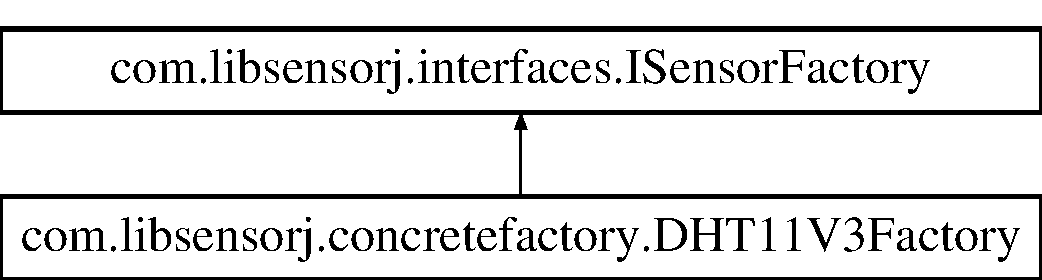
\includegraphics[height=2.000000cm]{classcom_1_1libsensorj_1_1concretefactory_1_1DHT11V3Factory}
\end{center}
\end{figure}
\subsection*{Public Member Functions}
\begin{DoxyCompactItemize}
\item 
\hyperlink{interfacecom_1_1libsensorj_1_1interfaces_1_1ISensor}{I\+Sensor} \hyperlink{classcom_1_1libsensorj_1_1concretefactory_1_1DHT11V3Factory_ad89c967025d654490729d2f69438805e}{create\+Sensor} ()
\item 
\hyperlink{classcom_1_1libsensorj_1_1interfaces_1_1IEvent}{I\+Event} \hyperlink{classcom_1_1libsensorj_1_1concretefactory_1_1DHT11V3Factory_a7621f6dc5c877e6dfb160f68e50fd319}{create\+Event} ()
\end{DoxyCompactItemize}


\subsection{Detailed Description}
A factory for creating D\+H\+T11\+V3 objects. 

\subsection{Member Function Documentation}
\hypertarget{classcom_1_1libsensorj_1_1concretefactory_1_1DHT11V3Factory_a7621f6dc5c877e6dfb160f68e50fd319}{}\index{com\+::libsensorj\+::concretefactory\+::\+D\+H\+T11\+V3\+Factory@{com\+::libsensorj\+::concretefactory\+::\+D\+H\+T11\+V3\+Factory}!create\+Event@{create\+Event}}
\index{create\+Event@{create\+Event}!com\+::libsensorj\+::concretefactory\+::\+D\+H\+T11\+V3\+Factory@{com\+::libsensorj\+::concretefactory\+::\+D\+H\+T11\+V3\+Factory}}
\subsubsection[{create\+Event}]{\setlength{\rightskip}{0pt plus 5cm}{\bf I\+Event} com.\+libsensorj.\+concretefactory.\+D\+H\+T11\+V3\+Factory.\+create\+Event (
\begin{DoxyParamCaption}
{}
\end{DoxyParamCaption}
)}\label{classcom_1_1libsensorj_1_1concretefactory_1_1DHT11V3Factory_a7621f6dc5c877e6dfb160f68e50fd319}
Creates a new I\+Event object.

\begin{DoxyReturn}{Returns}
the I\+Event 
\end{DoxyReturn}


Implements \hyperlink{interfacecom_1_1libsensorj_1_1interfaces_1_1ISensorFactory_a2b074d01287a4e64677097255ba9e768}{com.\+libsensorj.\+interfaces.\+I\+Sensor\+Factory}.

\hypertarget{classcom_1_1libsensorj_1_1concretefactory_1_1DHT11V3Factory_ad89c967025d654490729d2f69438805e}{}\index{com\+::libsensorj\+::concretefactory\+::\+D\+H\+T11\+V3\+Factory@{com\+::libsensorj\+::concretefactory\+::\+D\+H\+T11\+V3\+Factory}!create\+Sensor@{create\+Sensor}}
\index{create\+Sensor@{create\+Sensor}!com\+::libsensorj\+::concretefactory\+::\+D\+H\+T11\+V3\+Factory@{com\+::libsensorj\+::concretefactory\+::\+D\+H\+T11\+V3\+Factory}}
\subsubsection[{create\+Sensor}]{\setlength{\rightskip}{0pt plus 5cm}{\bf I\+Sensor} com.\+libsensorj.\+concretefactory.\+D\+H\+T11\+V3\+Factory.\+create\+Sensor (
\begin{DoxyParamCaption}
{}
\end{DoxyParamCaption}
)}\label{classcom_1_1libsensorj_1_1concretefactory_1_1DHT11V3Factory_ad89c967025d654490729d2f69438805e}
Creates a new I\+Sensor object.

\begin{DoxyReturn}{Returns}
the I\+Sensor 
\end{DoxyReturn}


Implements \hyperlink{interfacecom_1_1libsensorj_1_1interfaces_1_1ISensorFactory_ac14c6d566c37c6a79c6db1e85634f25d}{com.\+libsensorj.\+interfaces.\+I\+Sensor\+Factory}.



The documentation for this class was generated from the following file\+:\begin{DoxyCompactItemize}
\item 
main/java/com/libsensorj/concretefactory/\hyperlink{DHT11V3Factory_8java}{D\+H\+T11\+V3\+Factory.\+java}\end{DoxyCompactItemize}

\hypertarget{classcom_1_1libsensorj_1_1concretesensor_1_1HCSR04Device}{}\section{com.\+libsensorj.\+concretesensor.\+H\+C\+S\+R04\+Device Class Reference}
\label{classcom_1_1libsensorj_1_1concretesensor_1_1HCSR04Device}\index{com.\+libsensorj.\+concretesensor.\+H\+C\+S\+R04\+Device@{com.\+libsensorj.\+concretesensor.\+H\+C\+S\+R04\+Device}}
Inheritance diagram for com.\+libsensorj.\+concretesensor.\+H\+C\+S\+R04\+Device\+:\begin{figure}[H]
\begin{center}
\leavevmode
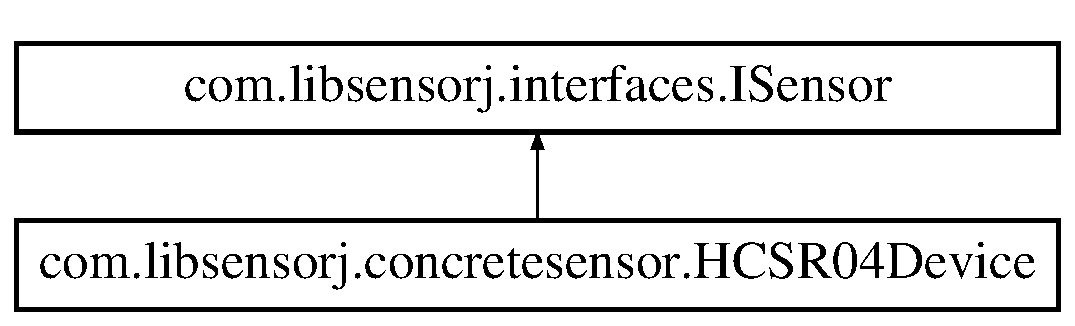
\includegraphics[height=2.000000cm]{classcom_1_1libsensorj_1_1concretesensor_1_1HCSR04Device}
\end{center}
\end{figure}
\subsection*{Public Member Functions}
\begin{DoxyCompactItemize}
\item 
\hyperlink{classcom_1_1libsensorj_1_1concretesensor_1_1HCSR04Device_ae0c7cdd02e374f360dff8d06a59b7c6d}{H\+C\+S\+R04\+Device} ()
\item 
\hyperlink{classcom_1_1libsensorj_1_1concretesensor_1_1HCSR04Device_a1c5c889b5ffe83c5fe8f7263bb8c8d33}{H\+C\+S\+R04\+Device} (int \+\_\+trigger, int \+\_\+echo)
\item 
\hyperlink{classcom_1_1libsensorj_1_1concretesensor_1_1HCSR04Device_a5148b245ef2aa510af815ecb3aeeb18b}{H\+C\+S\+R04\+Device} (Pin \+\_\+trigger, Pin \+\_\+echo)
\item 
void \hyperlink{classcom_1_1libsensorj_1_1concretesensor_1_1HCSR04Device_a3395de7d81b875516fb5c539accb27d1}{get\+Instance} ()
\item 
double \hyperlink{classcom_1_1libsensorj_1_1concretesensor_1_1HCSR04Device_aa30e4f6775819a36bc231a226c397bef}{get\+Distance} ()
\item 
void \hyperlink{classcom_1_1libsensorj_1_1concretesensor_1_1HCSR04Device_a69a3472b508507649ccb57e6fef81d6c}{close} ()
\end{DoxyCompactItemize}
\subsection*{Private Attributes}
\begin{DoxyCompactItemize}
\item 
Gpio\+Pin\+Digital\+Output \hyperlink{classcom_1_1libsensorj_1_1concretesensor_1_1HCSR04Device_ac898198f98143f7a1a4f281ea3c7c607}{trigger} = null
\item 
Gpio\+Pin\+Digital\+Input \hyperlink{classcom_1_1libsensorj_1_1concretesensor_1_1HCSR04Device_adf8ec00f094aefba690583e5a349c99d}{echo} = null
\end{DoxyCompactItemize}
\subsection*{Static Private Attributes}
\begin{DoxyCompactItemize}
\item 
static final int \hyperlink{classcom_1_1libsensorj_1_1concretesensor_1_1HCSR04Device_a1468a6c38c0086477a54eddbfe288299}{S\+P\+E\+E\+D\+O\+F\+S\+O\+U\+N\+D} = 34029
\item 
static final int \hyperlink{classcom_1_1libsensorj_1_1concretesensor_1_1HCSR04Device_a8f69accf3efa61a642b5e8693f7f158a}{T\+W\+O} = 2
\item 
static final long \hyperlink{classcom_1_1libsensorj_1_1concretesensor_1_1HCSR04Device_aaa527e39259b9e1be1b6360a397b3d30}{P\+U\+L\+S\+E\+\_\+\+T\+I\+M\+E} = 1
\item 
static final long \hyperlink{classcom_1_1libsensorj_1_1concretesensor_1_1HCSR04Device_a70071e4956bf93391031789b18039b6c}{D\+E\+L\+A\+Y} = 1000000000\+L
\item 
static final Logger \hyperlink{classcom_1_1libsensorj_1_1concretesensor_1_1HCSR04Device_a53449c0a7229928ddbb88c0d586cc63d}{L\+O\+G\+G\+E\+R}
\end{DoxyCompactItemize}


\subsection{Detailed Description}
The Class \hyperlink{classcom_1_1libsensorj_1_1concretesensor_1_1HCSR04Device}{H\+C\+S\+R04\+Device}. 

\subsection{Constructor \& Destructor Documentation}
\hypertarget{classcom_1_1libsensorj_1_1concretesensor_1_1HCSR04Device_ae0c7cdd02e374f360dff8d06a59b7c6d}{}\index{com\+::libsensorj\+::concretesensor\+::\+H\+C\+S\+R04\+Device@{com\+::libsensorj\+::concretesensor\+::\+H\+C\+S\+R04\+Device}!H\+C\+S\+R04\+Device@{H\+C\+S\+R04\+Device}}
\index{H\+C\+S\+R04\+Device@{H\+C\+S\+R04\+Device}!com\+::libsensorj\+::concretesensor\+::\+H\+C\+S\+R04\+Device@{com\+::libsensorj\+::concretesensor\+::\+H\+C\+S\+R04\+Device}}
\subsubsection[{H\+C\+S\+R04\+Device}]{\setlength{\rightskip}{0pt plus 5cm}com.\+libsensorj.\+concretesensor.\+H\+C\+S\+R04\+Device.\+H\+C\+S\+R04\+Device (
\begin{DoxyParamCaption}
{}
\end{DoxyParamCaption}
)}\label{classcom_1_1libsensorj_1_1concretesensor_1_1HCSR04Device_ae0c7cdd02e374f360dff8d06a59b7c6d}
Instantiates a new H\+C\+S r04 device. \hypertarget{classcom_1_1libsensorj_1_1concretesensor_1_1HCSR04Device_a1c5c889b5ffe83c5fe8f7263bb8c8d33}{}\index{com\+::libsensorj\+::concretesensor\+::\+H\+C\+S\+R04\+Device@{com\+::libsensorj\+::concretesensor\+::\+H\+C\+S\+R04\+Device}!H\+C\+S\+R04\+Device@{H\+C\+S\+R04\+Device}}
\index{H\+C\+S\+R04\+Device@{H\+C\+S\+R04\+Device}!com\+::libsensorj\+::concretesensor\+::\+H\+C\+S\+R04\+Device@{com\+::libsensorj\+::concretesensor\+::\+H\+C\+S\+R04\+Device}}
\subsubsection[{H\+C\+S\+R04\+Device}]{\setlength{\rightskip}{0pt plus 5cm}com.\+libsensorj.\+concretesensor.\+H\+C\+S\+R04\+Device.\+H\+C\+S\+R04\+Device (
\begin{DoxyParamCaption}
\item[{int}]{\+\_\+trigger, }
\item[{int}]{\+\_\+echo}
\end{DoxyParamCaption}
)}\label{classcom_1_1libsensorj_1_1concretesensor_1_1HCSR04Device_a1c5c889b5ffe83c5fe8f7263bb8c8d33}
Instantiates a new H\+C\+S r04 device.


\begin{DoxyParams}{Parameters}
{\em \+\_\+trigger} & the trigger \\
\hline
{\em \+\_\+echo} & the echo \\
\hline
\end{DoxyParams}
\hypertarget{classcom_1_1libsensorj_1_1concretesensor_1_1HCSR04Device_a5148b245ef2aa510af815ecb3aeeb18b}{}\index{com\+::libsensorj\+::concretesensor\+::\+H\+C\+S\+R04\+Device@{com\+::libsensorj\+::concretesensor\+::\+H\+C\+S\+R04\+Device}!H\+C\+S\+R04\+Device@{H\+C\+S\+R04\+Device}}
\index{H\+C\+S\+R04\+Device@{H\+C\+S\+R04\+Device}!com\+::libsensorj\+::concretesensor\+::\+H\+C\+S\+R04\+Device@{com\+::libsensorj\+::concretesensor\+::\+H\+C\+S\+R04\+Device}}
\subsubsection[{H\+C\+S\+R04\+Device}]{\setlength{\rightskip}{0pt plus 5cm}com.\+libsensorj.\+concretesensor.\+H\+C\+S\+R04\+Device.\+H\+C\+S\+R04\+Device (
\begin{DoxyParamCaption}
\item[{Pin}]{\+\_\+trigger, }
\item[{Pin}]{\+\_\+echo}
\end{DoxyParamCaption}
)}\label{classcom_1_1libsensorj_1_1concretesensor_1_1HCSR04Device_a5148b245ef2aa510af815ecb3aeeb18b}
Instantiates a new H\+C\+S r04 device.


\begin{DoxyParams}{Parameters}
{\em \+\_\+trigger} & the \+\_\+trigger \\
\hline
{\em \+\_\+echo} & the \+\_\+echo \\
\hline
\end{DoxyParams}


\subsection{Member Function Documentation}
\hypertarget{classcom_1_1libsensorj_1_1concretesensor_1_1HCSR04Device_a69a3472b508507649ccb57e6fef81d6c}{}\index{com\+::libsensorj\+::concretesensor\+::\+H\+C\+S\+R04\+Device@{com\+::libsensorj\+::concretesensor\+::\+H\+C\+S\+R04\+Device}!close@{close}}
\index{close@{close}!com\+::libsensorj\+::concretesensor\+::\+H\+C\+S\+R04\+Device@{com\+::libsensorj\+::concretesensor\+::\+H\+C\+S\+R04\+Device}}
\subsubsection[{close}]{\setlength{\rightskip}{0pt plus 5cm}void com.\+libsensorj.\+concretesensor.\+H\+C\+S\+R04\+Device.\+close (
\begin{DoxyParamCaption}
{}
\end{DoxyParamCaption}
)}\label{classcom_1_1libsensorj_1_1concretesensor_1_1HCSR04Device_a69a3472b508507649ccb57e6fef81d6c}
Close. \hypertarget{classcom_1_1libsensorj_1_1concretesensor_1_1HCSR04Device_aa30e4f6775819a36bc231a226c397bef}{}\index{com\+::libsensorj\+::concretesensor\+::\+H\+C\+S\+R04\+Device@{com\+::libsensorj\+::concretesensor\+::\+H\+C\+S\+R04\+Device}!get\+Distance@{get\+Distance}}
\index{get\+Distance@{get\+Distance}!com\+::libsensorj\+::concretesensor\+::\+H\+C\+S\+R04\+Device@{com\+::libsensorj\+::concretesensor\+::\+H\+C\+S\+R04\+Device}}
\subsubsection[{get\+Distance}]{\setlength{\rightskip}{0pt plus 5cm}double com.\+libsensorj.\+concretesensor.\+H\+C\+S\+R04\+Device.\+get\+Distance (
\begin{DoxyParamCaption}
{}
\end{DoxyParamCaption}
)}\label{classcom_1_1libsensorj_1_1concretesensor_1_1HCSR04Device_aa30e4f6775819a36bc231a226c397bef}
Gets the distance.

\begin{DoxyReturn}{Returns}
the distance 
\end{DoxyReturn}
\hypertarget{classcom_1_1libsensorj_1_1concretesensor_1_1HCSR04Device_a3395de7d81b875516fb5c539accb27d1}{}\index{com\+::libsensorj\+::concretesensor\+::\+H\+C\+S\+R04\+Device@{com\+::libsensorj\+::concretesensor\+::\+H\+C\+S\+R04\+Device}!get\+Instance@{get\+Instance}}
\index{get\+Instance@{get\+Instance}!com\+::libsensorj\+::concretesensor\+::\+H\+C\+S\+R04\+Device@{com\+::libsensorj\+::concretesensor\+::\+H\+C\+S\+R04\+Device}}
\subsubsection[{get\+Instance}]{\setlength{\rightskip}{0pt plus 5cm}void com.\+libsensorj.\+concretesensor.\+H\+C\+S\+R04\+Device.\+get\+Instance (
\begin{DoxyParamCaption}
{}
\end{DoxyParamCaption}
)}\label{classcom_1_1libsensorj_1_1concretesensor_1_1HCSR04Device_a3395de7d81b875516fb5c539accb27d1}
Gets the single instance of I\+Sensor.

\begin{DoxyReturn}{Returns}
single instance of I\+Sensor 
\end{DoxyReturn}


Implements \hyperlink{interfacecom_1_1libsensorj_1_1interfaces_1_1ISensor_a3c3db93a33adecde81a528651790f75e}{com.\+libsensorj.\+interfaces.\+I\+Sensor}.



\subsection{Member Data Documentation}
\hypertarget{classcom_1_1libsensorj_1_1concretesensor_1_1HCSR04Device_a70071e4956bf93391031789b18039b6c}{}\index{com\+::libsensorj\+::concretesensor\+::\+H\+C\+S\+R04\+Device@{com\+::libsensorj\+::concretesensor\+::\+H\+C\+S\+R04\+Device}!D\+E\+L\+A\+Y@{D\+E\+L\+A\+Y}}
\index{D\+E\+L\+A\+Y@{D\+E\+L\+A\+Y}!com\+::libsensorj\+::concretesensor\+::\+H\+C\+S\+R04\+Device@{com\+::libsensorj\+::concretesensor\+::\+H\+C\+S\+R04\+Device}}
\subsubsection[{D\+E\+L\+A\+Y}]{\setlength{\rightskip}{0pt plus 5cm}final long com.\+libsensorj.\+concretesensor.\+H\+C\+S\+R04\+Device.\+D\+E\+L\+A\+Y = 1000000000\+L\hspace{0.3cm}{\ttfamily [static]}, {\ttfamily [private]}}\label{classcom_1_1libsensorj_1_1concretesensor_1_1HCSR04Device_a70071e4956bf93391031789b18039b6c}
The Constant D\+E\+L\+A\+Y. \hypertarget{classcom_1_1libsensorj_1_1concretesensor_1_1HCSR04Device_adf8ec00f094aefba690583e5a349c99d}{}\index{com\+::libsensorj\+::concretesensor\+::\+H\+C\+S\+R04\+Device@{com\+::libsensorj\+::concretesensor\+::\+H\+C\+S\+R04\+Device}!echo@{echo}}
\index{echo@{echo}!com\+::libsensorj\+::concretesensor\+::\+H\+C\+S\+R04\+Device@{com\+::libsensorj\+::concretesensor\+::\+H\+C\+S\+R04\+Device}}
\subsubsection[{echo}]{\setlength{\rightskip}{0pt plus 5cm}Gpio\+Pin\+Digital\+Input com.\+libsensorj.\+concretesensor.\+H\+C\+S\+R04\+Device.\+echo = null\hspace{0.3cm}{\ttfamily [private]}}\label{classcom_1_1libsensorj_1_1concretesensor_1_1HCSR04Device_adf8ec00f094aefba690583e5a349c99d}
The echo. \hypertarget{classcom_1_1libsensorj_1_1concretesensor_1_1HCSR04Device_a53449c0a7229928ddbb88c0d586cc63d}{}\index{com\+::libsensorj\+::concretesensor\+::\+H\+C\+S\+R04\+Device@{com\+::libsensorj\+::concretesensor\+::\+H\+C\+S\+R04\+Device}!L\+O\+G\+G\+E\+R@{L\+O\+G\+G\+E\+R}}
\index{L\+O\+G\+G\+E\+R@{L\+O\+G\+G\+E\+R}!com\+::libsensorj\+::concretesensor\+::\+H\+C\+S\+R04\+Device@{com\+::libsensorj\+::concretesensor\+::\+H\+C\+S\+R04\+Device}}
\subsubsection[{L\+O\+G\+G\+E\+R}]{\setlength{\rightskip}{0pt plus 5cm}final Logger com.\+libsensorj.\+concretesensor.\+H\+C\+S\+R04\+Device.\+L\+O\+G\+G\+E\+R\hspace{0.3cm}{\ttfamily [static]}, {\ttfamily [private]}}\label{classcom_1_1libsensorj_1_1concretesensor_1_1HCSR04Device_a53449c0a7229928ddbb88c0d586cc63d}
{\bfseries Initial value\+:}
\begin{DoxyCode}
= LogManager
            .getLogger(\hyperlink{classcom_1_1libsensorj_1_1concretesensor_1_1HCSR04Device_ae0c7cdd02e374f360dff8d06a59b7c6d}{HCSR04Device}.class.getName())
\end{DoxyCode}
The Constant L\+O\+G\+G\+E\+R. \hypertarget{classcom_1_1libsensorj_1_1concretesensor_1_1HCSR04Device_aaa527e39259b9e1be1b6360a397b3d30}{}\index{com\+::libsensorj\+::concretesensor\+::\+H\+C\+S\+R04\+Device@{com\+::libsensorj\+::concretesensor\+::\+H\+C\+S\+R04\+Device}!P\+U\+L\+S\+E\+\_\+\+T\+I\+M\+E@{P\+U\+L\+S\+E\+\_\+\+T\+I\+M\+E}}
\index{P\+U\+L\+S\+E\+\_\+\+T\+I\+M\+E@{P\+U\+L\+S\+E\+\_\+\+T\+I\+M\+E}!com\+::libsensorj\+::concretesensor\+::\+H\+C\+S\+R04\+Device@{com\+::libsensorj\+::concretesensor\+::\+H\+C\+S\+R04\+Device}}
\subsubsection[{P\+U\+L\+S\+E\+\_\+\+T\+I\+M\+E}]{\setlength{\rightskip}{0pt plus 5cm}final long com.\+libsensorj.\+concretesensor.\+H\+C\+S\+R04\+Device.\+P\+U\+L\+S\+E\+\_\+\+T\+I\+M\+E = 1\hspace{0.3cm}{\ttfamily [static]}, {\ttfamily [private]}}\label{classcom_1_1libsensorj_1_1concretesensor_1_1HCSR04Device_aaa527e39259b9e1be1b6360a397b3d30}
The Constant P\+U\+L\+S\+E\+\_\+\+T\+I\+M\+E. \hypertarget{classcom_1_1libsensorj_1_1concretesensor_1_1HCSR04Device_a1468a6c38c0086477a54eddbfe288299}{}\index{com\+::libsensorj\+::concretesensor\+::\+H\+C\+S\+R04\+Device@{com\+::libsensorj\+::concretesensor\+::\+H\+C\+S\+R04\+Device}!S\+P\+E\+E\+D\+O\+F\+S\+O\+U\+N\+D@{S\+P\+E\+E\+D\+O\+F\+S\+O\+U\+N\+D}}
\index{S\+P\+E\+E\+D\+O\+F\+S\+O\+U\+N\+D@{S\+P\+E\+E\+D\+O\+F\+S\+O\+U\+N\+D}!com\+::libsensorj\+::concretesensor\+::\+H\+C\+S\+R04\+Device@{com\+::libsensorj\+::concretesensor\+::\+H\+C\+S\+R04\+Device}}
\subsubsection[{S\+P\+E\+E\+D\+O\+F\+S\+O\+U\+N\+D}]{\setlength{\rightskip}{0pt plus 5cm}final int com.\+libsensorj.\+concretesensor.\+H\+C\+S\+R04\+Device.\+S\+P\+E\+E\+D\+O\+F\+S\+O\+U\+N\+D = 34029\hspace{0.3cm}{\ttfamily [static]}, {\ttfamily [private]}}\label{classcom_1_1libsensorj_1_1concretesensor_1_1HCSR04Device_a1468a6c38c0086477a54eddbfe288299}
The Constant S\+P\+E\+E\+D\+O\+F\+S\+O\+U\+N\+D. \hypertarget{classcom_1_1libsensorj_1_1concretesensor_1_1HCSR04Device_ac898198f98143f7a1a4f281ea3c7c607}{}\index{com\+::libsensorj\+::concretesensor\+::\+H\+C\+S\+R04\+Device@{com\+::libsensorj\+::concretesensor\+::\+H\+C\+S\+R04\+Device}!trigger@{trigger}}
\index{trigger@{trigger}!com\+::libsensorj\+::concretesensor\+::\+H\+C\+S\+R04\+Device@{com\+::libsensorj\+::concretesensor\+::\+H\+C\+S\+R04\+Device}}
\subsubsection[{trigger}]{\setlength{\rightskip}{0pt plus 5cm}Gpio\+Pin\+Digital\+Output com.\+libsensorj.\+concretesensor.\+H\+C\+S\+R04\+Device.\+trigger = null\hspace{0.3cm}{\ttfamily [private]}}\label{classcom_1_1libsensorj_1_1concretesensor_1_1HCSR04Device_ac898198f98143f7a1a4f281ea3c7c607}
The trigger. \hypertarget{classcom_1_1libsensorj_1_1concretesensor_1_1HCSR04Device_a8f69accf3efa61a642b5e8693f7f158a}{}\index{com\+::libsensorj\+::concretesensor\+::\+H\+C\+S\+R04\+Device@{com\+::libsensorj\+::concretesensor\+::\+H\+C\+S\+R04\+Device}!T\+W\+O@{T\+W\+O}}
\index{T\+W\+O@{T\+W\+O}!com\+::libsensorj\+::concretesensor\+::\+H\+C\+S\+R04\+Device@{com\+::libsensorj\+::concretesensor\+::\+H\+C\+S\+R04\+Device}}
\subsubsection[{T\+W\+O}]{\setlength{\rightskip}{0pt plus 5cm}final int com.\+libsensorj.\+concretesensor.\+H\+C\+S\+R04\+Device.\+T\+W\+O = 2\hspace{0.3cm}{\ttfamily [static]}, {\ttfamily [private]}}\label{classcom_1_1libsensorj_1_1concretesensor_1_1HCSR04Device_a8f69accf3efa61a642b5e8693f7f158a}
The Constant T\+W\+O. 

The documentation for this class was generated from the following file\+:\begin{DoxyCompactItemize}
\item 
main/java/com/libsensorj/concretesensor/\hyperlink{HCSR04Device_8java}{H\+C\+S\+R04\+Device.\+java}\end{DoxyCompactItemize}

\hypertarget{classcom_1_1libsensorj_1_1examples_1_1HCSR04DeviceExample}{}\section{com.\+libsensorj.\+examples.\+H\+C\+S\+R04\+Device\+Example Class Reference}
\label{classcom_1_1libsensorj_1_1examples_1_1HCSR04DeviceExample}\index{com.\+libsensorj.\+examples.\+H\+C\+S\+R04\+Device\+Example@{com.\+libsensorj.\+examples.\+H\+C\+S\+R04\+Device\+Example}}
\subsection*{Static Public Member Functions}
\begin{DoxyCompactItemize}
\item 
static void \hyperlink{classcom_1_1libsensorj_1_1examples_1_1HCSR04DeviceExample_ab213367036bb78e1b6614967207a718a}{main} (String\mbox{[}$\,$\mbox{]} args)
\end{DoxyCompactItemize}
\subsection*{Static Private Attributes}
\begin{DoxyCompactItemize}
\item 
static \hyperlink{interfacecom_1_1libsensorj_1_1interfaces_1_1ISensor}{I\+Sensor} \hyperlink{classcom_1_1libsensorj_1_1examples_1_1HCSR04DeviceExample_aa4f457230d5989c781e4c142492cf9c2}{hcsr}
\item 
static final Logger \hyperlink{classcom_1_1libsensorj_1_1examples_1_1HCSR04DeviceExample_a156f69717cfae755de776e6310ae212f}{L\+O\+G\+G\+E\+R}
\end{DoxyCompactItemize}


\subsection{Detailed Description}
The Class \hyperlink{classcom_1_1libsensorj_1_1examples_1_1HCSR04DeviceExample}{H\+C\+S\+R04\+Device\+Example}. 

\subsection{Member Function Documentation}
\hypertarget{classcom_1_1libsensorj_1_1examples_1_1HCSR04DeviceExample_ab213367036bb78e1b6614967207a718a}{}\index{com\+::libsensorj\+::examples\+::\+H\+C\+S\+R04\+Device\+Example@{com\+::libsensorj\+::examples\+::\+H\+C\+S\+R04\+Device\+Example}!main@{main}}
\index{main@{main}!com\+::libsensorj\+::examples\+::\+H\+C\+S\+R04\+Device\+Example@{com\+::libsensorj\+::examples\+::\+H\+C\+S\+R04\+Device\+Example}}
\subsubsection[{main}]{\setlength{\rightskip}{0pt plus 5cm}static void com.\+libsensorj.\+examples.\+H\+C\+S\+R04\+Device\+Example.\+main (
\begin{DoxyParamCaption}
\item[{String\mbox{[}$\,$\mbox{]}}]{args}
\end{DoxyParamCaption}
)\hspace{0.3cm}{\ttfamily [static]}}\label{classcom_1_1libsensorj_1_1examples_1_1HCSR04DeviceExample_ab213367036bb78e1b6614967207a718a}
The main method.


\begin{DoxyParams}{Parameters}
{\em args} & the arguments \\
\hline
\end{DoxyParams}


\subsection{Member Data Documentation}
\hypertarget{classcom_1_1libsensorj_1_1examples_1_1HCSR04DeviceExample_aa4f457230d5989c781e4c142492cf9c2}{}\index{com\+::libsensorj\+::examples\+::\+H\+C\+S\+R04\+Device\+Example@{com\+::libsensorj\+::examples\+::\+H\+C\+S\+R04\+Device\+Example}!hcsr@{hcsr}}
\index{hcsr@{hcsr}!com\+::libsensorj\+::examples\+::\+H\+C\+S\+R04\+Device\+Example@{com\+::libsensorj\+::examples\+::\+H\+C\+S\+R04\+Device\+Example}}
\subsubsection[{hcsr}]{\setlength{\rightskip}{0pt plus 5cm}{\bf I\+Sensor} com.\+libsensorj.\+examples.\+H\+C\+S\+R04\+Device\+Example.\+hcsr\hspace{0.3cm}{\ttfamily [static]}, {\ttfamily [private]}}\label{classcom_1_1libsensorj_1_1examples_1_1HCSR04DeviceExample_aa4f457230d5989c781e4c142492cf9c2}
The I\+Sensor hcsr. \hypertarget{classcom_1_1libsensorj_1_1examples_1_1HCSR04DeviceExample_a156f69717cfae755de776e6310ae212f}{}\index{com\+::libsensorj\+::examples\+::\+H\+C\+S\+R04\+Device\+Example@{com\+::libsensorj\+::examples\+::\+H\+C\+S\+R04\+Device\+Example}!L\+O\+G\+G\+E\+R@{L\+O\+G\+G\+E\+R}}
\index{L\+O\+G\+G\+E\+R@{L\+O\+G\+G\+E\+R}!com\+::libsensorj\+::examples\+::\+H\+C\+S\+R04\+Device\+Example@{com\+::libsensorj\+::examples\+::\+H\+C\+S\+R04\+Device\+Example}}
\subsubsection[{L\+O\+G\+G\+E\+R}]{\setlength{\rightskip}{0pt plus 5cm}final Logger com.\+libsensorj.\+examples.\+H\+C\+S\+R04\+Device\+Example.\+L\+O\+G\+G\+E\+R\hspace{0.3cm}{\ttfamily [static]}, {\ttfamily [private]}}\label{classcom_1_1libsensorj_1_1examples_1_1HCSR04DeviceExample_a156f69717cfae755de776e6310ae212f}
{\bfseries Initial value\+:}
\begin{DoxyCode}
= LogManager
            .getLogger(HCSR04DeviceExample.class.getName())
\end{DoxyCode}
The Constant L\+O\+G\+G\+E\+R. 

The documentation for this class was generated from the following file\+:\begin{DoxyCompactItemize}
\item 
main/java/com/libsensorj/examples/\hyperlink{HCSR04DeviceExample_8java}{H\+C\+S\+R04\+Device\+Example.\+java}\end{DoxyCompactItemize}

\hypertarget{classcom_1_1libsensorj_1_1concretefactory_1_1HCSR04DeviceFactory}{}\section{com.\+libsensorj.\+concretefactory.\+H\+C\+S\+R04\+Device\+Factory Class Reference}
\label{classcom_1_1libsensorj_1_1concretefactory_1_1HCSR04DeviceFactory}\index{com.\+libsensorj.\+concretefactory.\+H\+C\+S\+R04\+Device\+Factory@{com.\+libsensorj.\+concretefactory.\+H\+C\+S\+R04\+Device\+Factory}}
Inheritance diagram for com.\+libsensorj.\+concretefactory.\+H\+C\+S\+R04\+Device\+Factory\+:\begin{figure}[H]
\begin{center}
\leavevmode
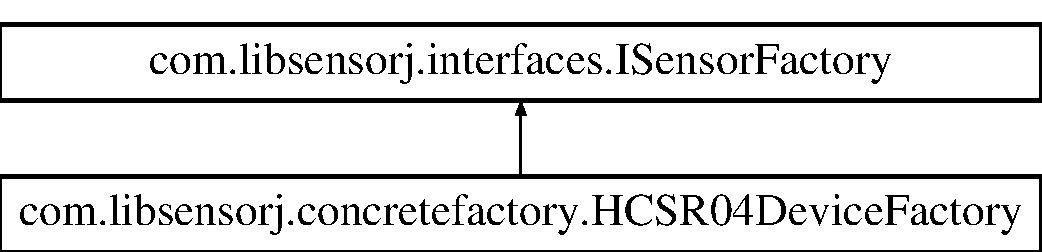
\includegraphics[height=2.000000cm]{classcom_1_1libsensorj_1_1concretefactory_1_1HCSR04DeviceFactory}
\end{center}
\end{figure}
\subsection*{Public Member Functions}
\begin{DoxyCompactItemize}
\item 
\hyperlink{interfacecom_1_1libsensorj_1_1interfaces_1_1ISensor}{I\+Sensor} \hyperlink{classcom_1_1libsensorj_1_1concretefactory_1_1HCSR04DeviceFactory_a3d5c07b9ce458a3f56cfe5e7470b51df}{create\+Sensor} ()
\item 
\hyperlink{classcom_1_1libsensorj_1_1interfaces_1_1IEvent}{I\+Event} \hyperlink{classcom_1_1libsensorj_1_1concretefactory_1_1HCSR04DeviceFactory_aea88b0202d3021c4e55bd9cbf64da906}{create\+Event} ()
\end{DoxyCompactItemize}


\subsection{Detailed Description}
A factory for creating H\+C\+S\+R04\+Device objects. 

\subsection{Member Function Documentation}
\hypertarget{classcom_1_1libsensorj_1_1concretefactory_1_1HCSR04DeviceFactory_aea88b0202d3021c4e55bd9cbf64da906}{}\index{com\+::libsensorj\+::concretefactory\+::\+H\+C\+S\+R04\+Device\+Factory@{com\+::libsensorj\+::concretefactory\+::\+H\+C\+S\+R04\+Device\+Factory}!create\+Event@{create\+Event}}
\index{create\+Event@{create\+Event}!com\+::libsensorj\+::concretefactory\+::\+H\+C\+S\+R04\+Device\+Factory@{com\+::libsensorj\+::concretefactory\+::\+H\+C\+S\+R04\+Device\+Factory}}
\subsubsection[{create\+Event}]{\setlength{\rightskip}{0pt plus 5cm}{\bf I\+Event} com.\+libsensorj.\+concretefactory.\+H\+C\+S\+R04\+Device\+Factory.\+create\+Event (
\begin{DoxyParamCaption}
{}
\end{DoxyParamCaption}
)}\label{classcom_1_1libsensorj_1_1concretefactory_1_1HCSR04DeviceFactory_aea88b0202d3021c4e55bd9cbf64da906}
Creates a new I\+Event object.

\begin{DoxyReturn}{Returns}
the I\+Event 
\end{DoxyReturn}


Implements \hyperlink{interfacecom_1_1libsensorj_1_1interfaces_1_1ISensorFactory_a2b074d01287a4e64677097255ba9e768}{com.\+libsensorj.\+interfaces.\+I\+Sensor\+Factory}.

\hypertarget{classcom_1_1libsensorj_1_1concretefactory_1_1HCSR04DeviceFactory_a3d5c07b9ce458a3f56cfe5e7470b51df}{}\index{com\+::libsensorj\+::concretefactory\+::\+H\+C\+S\+R04\+Device\+Factory@{com\+::libsensorj\+::concretefactory\+::\+H\+C\+S\+R04\+Device\+Factory}!create\+Sensor@{create\+Sensor}}
\index{create\+Sensor@{create\+Sensor}!com\+::libsensorj\+::concretefactory\+::\+H\+C\+S\+R04\+Device\+Factory@{com\+::libsensorj\+::concretefactory\+::\+H\+C\+S\+R04\+Device\+Factory}}
\subsubsection[{create\+Sensor}]{\setlength{\rightskip}{0pt plus 5cm}{\bf I\+Sensor} com.\+libsensorj.\+concretefactory.\+H\+C\+S\+R04\+Device\+Factory.\+create\+Sensor (
\begin{DoxyParamCaption}
{}
\end{DoxyParamCaption}
)}\label{classcom_1_1libsensorj_1_1concretefactory_1_1HCSR04DeviceFactory_a3d5c07b9ce458a3f56cfe5e7470b51df}
Creates a new I\+Sensor object.

\begin{DoxyReturn}{Returns}
the I\+Sensor 
\end{DoxyReturn}


Implements \hyperlink{interfacecom_1_1libsensorj_1_1interfaces_1_1ISensorFactory_ac14c6d566c37c6a79c6db1e85634f25d}{com.\+libsensorj.\+interfaces.\+I\+Sensor\+Factory}.



The documentation for this class was generated from the following file\+:\begin{DoxyCompactItemize}
\item 
main/java/com/libsensorj/concretefactory/\hyperlink{HCSR04DeviceFactory_8java}{H\+C\+S\+R04\+Device\+Factory.\+java}\end{DoxyCompactItemize}

\hypertarget{classcom_1_1libsensorj_1_1concreteevent_1_1HumidityEvent}{}\section{com.\+libsensorj.\+concreteevent.\+Humidity\+Event Class Reference}
\label{classcom_1_1libsensorj_1_1concreteevent_1_1HumidityEvent}\index{com.\+libsensorj.\+concreteevent.\+Humidity\+Event@{com.\+libsensorj.\+concreteevent.\+Humidity\+Event}}
Inheritance diagram for com.\+libsensorj.\+concreteevent.\+Humidity\+Event\+:\begin{figure}[H]
\begin{center}
\leavevmode
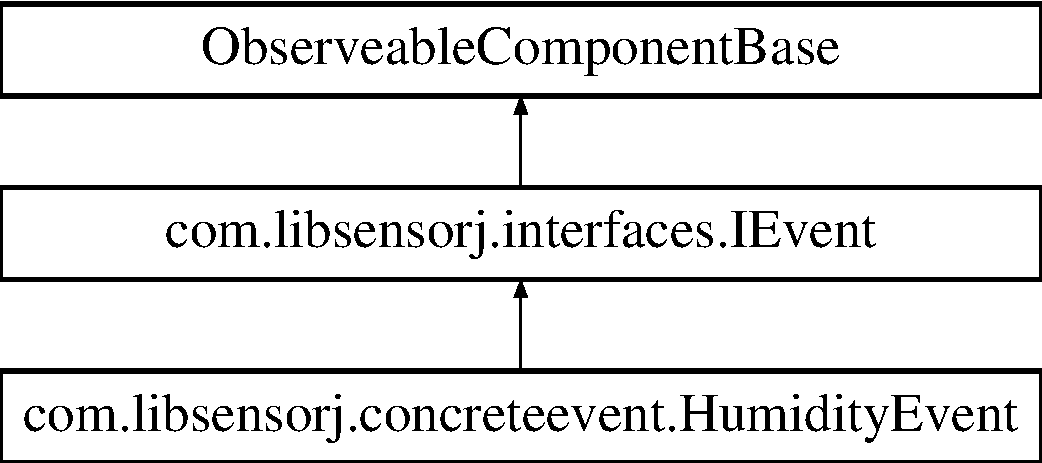
\includegraphics[height=2.000000cm]{classcom_1_1libsensorj_1_1concreteevent_1_1HumidityEvent}
\end{center}
\end{figure}
\subsection*{Public Member Functions}
\begin{DoxyCompactItemize}
\item 
void \hyperlink{classcom_1_1libsensorj_1_1concreteevent_1_1HumidityEvent_a4ea7f94d2402aeafca55dc1fb2950d00}{attach} (\hyperlink{classcom_1_1libsensorj_1_1model_1_1Observer}{Observer} obsever)
\item 
void \hyperlink{classcom_1_1libsensorj_1_1concreteevent_1_1HumidityEvent_a577a1f99a7993ccd8019fb46c1668c9b}{detach} (\hyperlink{classcom_1_1libsensorj_1_1model_1_1Observer}{Observer} obsever)
\item 
void \hyperlink{classcom_1_1libsensorj_1_1concreteevent_1_1HumidityEvent_ad3d8c57f1934c115f0c9374394d9a601}{trigger} ()
\end{DoxyCompactItemize}


\subsection{Member Function Documentation}
\hypertarget{classcom_1_1libsensorj_1_1concreteevent_1_1HumidityEvent_a4ea7f94d2402aeafca55dc1fb2950d00}{}\index{com\+::libsensorj\+::concreteevent\+::\+Humidity\+Event@{com\+::libsensorj\+::concreteevent\+::\+Humidity\+Event}!attach@{attach}}
\index{attach@{attach}!com\+::libsensorj\+::concreteevent\+::\+Humidity\+Event@{com\+::libsensorj\+::concreteevent\+::\+Humidity\+Event}}
\subsubsection[{attach}]{\setlength{\rightskip}{0pt plus 5cm}void com.\+libsensorj.\+concreteevent.\+Humidity\+Event.\+attach (
\begin{DoxyParamCaption}
\item[{{\bf Observer}}]{obsever}
\end{DoxyParamCaption}
)}\label{classcom_1_1libsensorj_1_1concreteevent_1_1HumidityEvent_a4ea7f94d2402aeafca55dc1fb2950d00}


Implements \hyperlink{interfacecom_1_1libsensorj_1_1interfaces_1_1IEvent_af5af4301ccb6670452419d68baddf372}{com.\+libsensorj.\+interfaces.\+I\+Event}.

\hypertarget{classcom_1_1libsensorj_1_1concreteevent_1_1HumidityEvent_a577a1f99a7993ccd8019fb46c1668c9b}{}\index{com\+::libsensorj\+::concreteevent\+::\+Humidity\+Event@{com\+::libsensorj\+::concreteevent\+::\+Humidity\+Event}!detach@{detach}}
\index{detach@{detach}!com\+::libsensorj\+::concreteevent\+::\+Humidity\+Event@{com\+::libsensorj\+::concreteevent\+::\+Humidity\+Event}}
\subsubsection[{detach}]{\setlength{\rightskip}{0pt plus 5cm}void com.\+libsensorj.\+concreteevent.\+Humidity\+Event.\+detach (
\begin{DoxyParamCaption}
\item[{{\bf Observer}}]{obsever}
\end{DoxyParamCaption}
)}\label{classcom_1_1libsensorj_1_1concreteevent_1_1HumidityEvent_a577a1f99a7993ccd8019fb46c1668c9b}


Implements \hyperlink{interfacecom_1_1libsensorj_1_1interfaces_1_1IEvent_a974b07df97fda9f3be8e4afcd46470b2}{com.\+libsensorj.\+interfaces.\+I\+Event}.

\hypertarget{classcom_1_1libsensorj_1_1concreteevent_1_1HumidityEvent_ad3d8c57f1934c115f0c9374394d9a601}{}\index{com\+::libsensorj\+::concreteevent\+::\+Humidity\+Event@{com\+::libsensorj\+::concreteevent\+::\+Humidity\+Event}!trigger@{trigger}}
\index{trigger@{trigger}!com\+::libsensorj\+::concreteevent\+::\+Humidity\+Event@{com\+::libsensorj\+::concreteevent\+::\+Humidity\+Event}}
\subsubsection[{trigger}]{\setlength{\rightskip}{0pt plus 5cm}void com.\+libsensorj.\+concreteevent.\+Humidity\+Event.\+trigger (
\begin{DoxyParamCaption}
{}
\end{DoxyParamCaption}
)}\label{classcom_1_1libsensorj_1_1concreteevent_1_1HumidityEvent_ad3d8c57f1934c115f0c9374394d9a601}


Implements \hyperlink{interfacecom_1_1libsensorj_1_1interfaces_1_1IEvent_a861dea0956f77dd82f95e0110b8043b2}{com.\+libsensorj.\+interfaces.\+I\+Event}.



The documentation for this class was generated from the following file\+:\begin{DoxyCompactItemize}
\item 
main/java/com/libsensorj/concreteevent/\hyperlink{HumidityEvent_8java}{Humidity\+Event.\+java}\end{DoxyCompactItemize}

\hypertarget{classcom_1_1libsensorj_1_1concretefactory_1_1HumiditySensorFactory}{}\section{com.\+libsensorj.\+concretefactory.\+Humidity\+Sensor\+Factory Class Reference}
\label{classcom_1_1libsensorj_1_1concretefactory_1_1HumiditySensorFactory}\index{com.\+libsensorj.\+concretefactory.\+Humidity\+Sensor\+Factory@{com.\+libsensorj.\+concretefactory.\+Humidity\+Sensor\+Factory}}
Inheritance diagram for com.\+libsensorj.\+concretefactory.\+Humidity\+Sensor\+Factory\+:\begin{figure}[H]
\begin{center}
\leavevmode
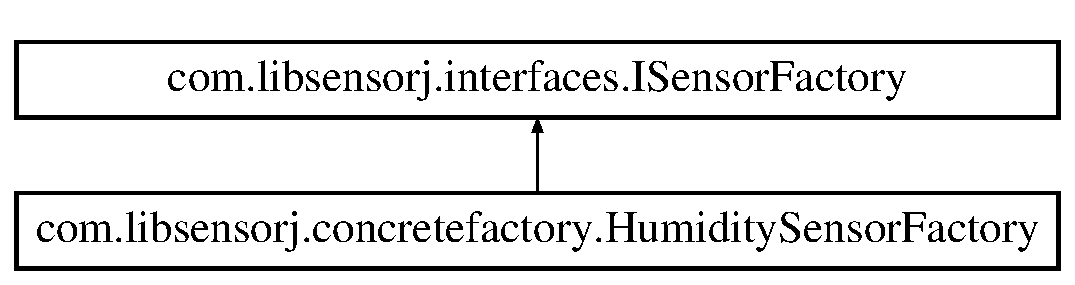
\includegraphics[height=2.000000cm]{classcom_1_1libsensorj_1_1concretefactory_1_1HumiditySensorFactory}
\end{center}
\end{figure}
\subsection*{Public Member Functions}
\begin{DoxyCompactItemize}
\item 
\hyperlink{interfacecom_1_1libsensorj_1_1interfaces_1_1ISensor}{I\+Sensor} \hyperlink{classcom_1_1libsensorj_1_1concretefactory_1_1HumiditySensorFactory_aec6f80bd08e69d69ea6187067d11d28c}{create\+Sensor} ()
\item 
\hyperlink{classcom_1_1libsensorj_1_1interfaces_1_1IEvent}{I\+Event} \hyperlink{classcom_1_1libsensorj_1_1concretefactory_1_1HumiditySensorFactory_a43835bfa4c60faf39dfe64f67322b9e4}{create\+Event} ()
\end{DoxyCompactItemize}


\subsection{Detailed Description}
A factory for creating Humidity\+Sensor objects. 

\subsection{Member Function Documentation}
\hypertarget{classcom_1_1libsensorj_1_1concretefactory_1_1HumiditySensorFactory_a43835bfa4c60faf39dfe64f67322b9e4}{}\index{com\+::libsensorj\+::concretefactory\+::\+Humidity\+Sensor\+Factory@{com\+::libsensorj\+::concretefactory\+::\+Humidity\+Sensor\+Factory}!create\+Event@{create\+Event}}
\index{create\+Event@{create\+Event}!com\+::libsensorj\+::concretefactory\+::\+Humidity\+Sensor\+Factory@{com\+::libsensorj\+::concretefactory\+::\+Humidity\+Sensor\+Factory}}
\subsubsection[{create\+Event}]{\setlength{\rightskip}{0pt plus 5cm}{\bf I\+Event} com.\+libsensorj.\+concretefactory.\+Humidity\+Sensor\+Factory.\+create\+Event (
\begin{DoxyParamCaption}
{}
\end{DoxyParamCaption}
)}\label{classcom_1_1libsensorj_1_1concretefactory_1_1HumiditySensorFactory_a43835bfa4c60faf39dfe64f67322b9e4}
Creates a new I\+Event object.

\begin{DoxyReturn}{Returns}
the I\+Event 
\end{DoxyReturn}


Implements \hyperlink{interfacecom_1_1libsensorj_1_1interfaces_1_1ISensorFactory_a2b074d01287a4e64677097255ba9e768}{com.\+libsensorj.\+interfaces.\+I\+Sensor\+Factory}.

\hypertarget{classcom_1_1libsensorj_1_1concretefactory_1_1HumiditySensorFactory_aec6f80bd08e69d69ea6187067d11d28c}{}\index{com\+::libsensorj\+::concretefactory\+::\+Humidity\+Sensor\+Factory@{com\+::libsensorj\+::concretefactory\+::\+Humidity\+Sensor\+Factory}!create\+Sensor@{create\+Sensor}}
\index{create\+Sensor@{create\+Sensor}!com\+::libsensorj\+::concretefactory\+::\+Humidity\+Sensor\+Factory@{com\+::libsensorj\+::concretefactory\+::\+Humidity\+Sensor\+Factory}}
\subsubsection[{create\+Sensor}]{\setlength{\rightskip}{0pt plus 5cm}{\bf I\+Sensor} com.\+libsensorj.\+concretefactory.\+Humidity\+Sensor\+Factory.\+create\+Sensor (
\begin{DoxyParamCaption}
{}
\end{DoxyParamCaption}
)}\label{classcom_1_1libsensorj_1_1concretefactory_1_1HumiditySensorFactory_aec6f80bd08e69d69ea6187067d11d28c}
Creates a new I\+Sensor object.

\begin{DoxyReturn}{Returns}
the I\+Sensor 
\end{DoxyReturn}


Implements \hyperlink{interfacecom_1_1libsensorj_1_1interfaces_1_1ISensorFactory_ac14c6d566c37c6a79c6db1e85634f25d}{com.\+libsensorj.\+interfaces.\+I\+Sensor\+Factory}.



The documentation for this class was generated from the following file\+:\begin{DoxyCompactItemize}
\item 
main/java/com/libsensorj/concretefactory/\hyperlink{HumiditySensorFactory_8java}{Humidity\+Sensor\+Factory.\+java}\end{DoxyCompactItemize}

\hypertarget{classcom_1_1libsensorj_1_1interfaces_1_1IEvent}{}\section{com.\+libsensorj.\+interfaces.\+I\+Event Class Reference}
\label{classcom_1_1libsensorj_1_1interfaces_1_1IEvent}\index{com.\+libsensorj.\+interfaces.\+I\+Event@{com.\+libsensorj.\+interfaces.\+I\+Event}}
Inheritance diagram for com.\+libsensorj.\+interfaces.\+I\+Event\+:\begin{figure}[H]
\begin{center}
\leavevmode
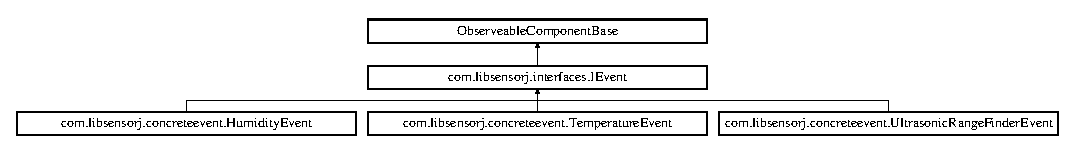
\includegraphics[height=1.595442cm]{classcom_1_1libsensorj_1_1interfaces_1_1IEvent}
\end{center}
\end{figure}
\subsection*{Public Member Functions}
\begin{DoxyCompactItemize}
\item 
abstract void \hyperlink{classcom_1_1libsensorj_1_1interfaces_1_1IEvent_a7e3cbdca3cceb9345483cf019760b113}{attach} (\hyperlink{classcom_1_1libsensorj_1_1model_1_1Observer}{Observer} obsever)
\item 
abstract void \hyperlink{classcom_1_1libsensorj_1_1interfaces_1_1IEvent_aae7d245feed8380465149bfa36724244}{detach} (\hyperlink{classcom_1_1libsensorj_1_1model_1_1Observer}{Observer} obsever)
\item 
abstract void \hyperlink{classcom_1_1libsensorj_1_1interfaces_1_1IEvent_aa12268158f158fbb805b558efeb1bb67}{trigger} ()
\end{DoxyCompactItemize}


\subsection{Detailed Description}
The Class \hyperlink{classcom_1_1libsensorj_1_1interfaces_1_1IEvent}{I\+Event}. 

\subsection{Member Function Documentation}
\hypertarget{classcom_1_1libsensorj_1_1interfaces_1_1IEvent_a7e3cbdca3cceb9345483cf019760b113}{}\index{com\+::libsensorj\+::interfaces\+::\+I\+Event@{com\+::libsensorj\+::interfaces\+::\+I\+Event}!attach@{attach}}
\index{attach@{attach}!com\+::libsensorj\+::interfaces\+::\+I\+Event@{com\+::libsensorj\+::interfaces\+::\+I\+Event}}
\subsubsection[{attach}]{\setlength{\rightskip}{0pt plus 5cm}abstract void com.\+libsensorj.\+interfaces.\+I\+Event.\+attach (
\begin{DoxyParamCaption}
\item[{{\bf Observer}}]{obsever}
\end{DoxyParamCaption}
)\hspace{0.3cm}{\ttfamily [abstract]}}\label{classcom_1_1libsensorj_1_1interfaces_1_1IEvent_a7e3cbdca3cceb9345483cf019760b113}
Attach.


\begin{DoxyParams}{Parameters}
{\em obsever} & the obsever \\
\hline
\end{DoxyParams}
\hypertarget{classcom_1_1libsensorj_1_1interfaces_1_1IEvent_aae7d245feed8380465149bfa36724244}{}\index{com\+::libsensorj\+::interfaces\+::\+I\+Event@{com\+::libsensorj\+::interfaces\+::\+I\+Event}!detach@{detach}}
\index{detach@{detach}!com\+::libsensorj\+::interfaces\+::\+I\+Event@{com\+::libsensorj\+::interfaces\+::\+I\+Event}}
\subsubsection[{detach}]{\setlength{\rightskip}{0pt plus 5cm}abstract void com.\+libsensorj.\+interfaces.\+I\+Event.\+detach (
\begin{DoxyParamCaption}
\item[{{\bf Observer}}]{obsever}
\end{DoxyParamCaption}
)\hspace{0.3cm}{\ttfamily [abstract]}}\label{classcom_1_1libsensorj_1_1interfaces_1_1IEvent_aae7d245feed8380465149bfa36724244}
Detach.


\begin{DoxyParams}{Parameters}
{\em obsever} & the obsever \\
\hline
\end{DoxyParams}
\hypertarget{classcom_1_1libsensorj_1_1interfaces_1_1IEvent_aa12268158f158fbb805b558efeb1bb67}{}\index{com\+::libsensorj\+::interfaces\+::\+I\+Event@{com\+::libsensorj\+::interfaces\+::\+I\+Event}!trigger@{trigger}}
\index{trigger@{trigger}!com\+::libsensorj\+::interfaces\+::\+I\+Event@{com\+::libsensorj\+::interfaces\+::\+I\+Event}}
\subsubsection[{trigger}]{\setlength{\rightskip}{0pt plus 5cm}abstract void com.\+libsensorj.\+interfaces.\+I\+Event.\+trigger (
\begin{DoxyParamCaption}
{}
\end{DoxyParamCaption}
)\hspace{0.3cm}{\ttfamily [abstract]}}\label{classcom_1_1libsensorj_1_1interfaces_1_1IEvent_aa12268158f158fbb805b558efeb1bb67}
Trigger. 

The documentation for this class was generated from the following file\+:\begin{DoxyCompactItemize}
\item 
main/java/com/libsensorj/interfaces/\hyperlink{IEvent_8java}{I\+Event.\+java}\end{DoxyCompactItemize}

\hypertarget{interfacecom_1_1libsensorj_1_1interfaces_1_1ISensor}{}\section{com.\+libsensorj.\+interfaces.\+I\+Sensor Interface Reference}
\label{interfacecom_1_1libsensorj_1_1interfaces_1_1ISensor}\index{com.\+libsensorj.\+interfaces.\+I\+Sensor@{com.\+libsensorj.\+interfaces.\+I\+Sensor}}
Inheritance diagram for com.\+libsensorj.\+interfaces.\+I\+Sensor\+:\begin{figure}[H]
\begin{center}
\leavevmode
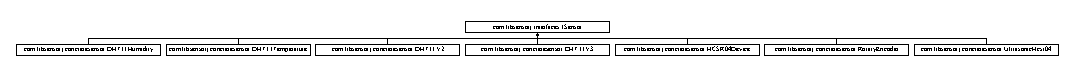
\includegraphics[height=1.216069cm]{interfacecom_1_1libsensorj_1_1interfaces_1_1ISensor}
\end{center}
\end{figure}
\subsection*{Public Member Functions}
\begin{DoxyCompactItemize}
\item 
void \hyperlink{interfacecom_1_1libsensorj_1_1interfaces_1_1ISensor_a3c3db93a33adecde81a528651790f75e}{get\+Instance} ()
\end{DoxyCompactItemize}


\subsection{Member Function Documentation}
\hypertarget{interfacecom_1_1libsensorj_1_1interfaces_1_1ISensor_a3c3db93a33adecde81a528651790f75e}{}\index{com\+::libsensorj\+::interfaces\+::\+I\+Sensor@{com\+::libsensorj\+::interfaces\+::\+I\+Sensor}!get\+Instance@{get\+Instance}}
\index{get\+Instance@{get\+Instance}!com\+::libsensorj\+::interfaces\+::\+I\+Sensor@{com\+::libsensorj\+::interfaces\+::\+I\+Sensor}}
\subsubsection[{get\+Instance}]{\setlength{\rightskip}{0pt plus 5cm}void com.\+libsensorj.\+interfaces.\+I\+Sensor.\+get\+Instance (
\begin{DoxyParamCaption}
{}
\end{DoxyParamCaption}
)}\label{interfacecom_1_1libsensorj_1_1interfaces_1_1ISensor_a3c3db93a33adecde81a528651790f75e}


Implemented in \hyperlink{classcom_1_1libsensorj_1_1concretesensor_1_1DHT11Temperature_a599358623598fb0076dc0a2e07978f0b}{com.\+libsensorj.\+concretesensor.\+D\+H\+T11\+Temperature}, \hyperlink{classcom_1_1libsensorj_1_1concretesensor_1_1UltrasonicHcsr04_a170167614b330d79518647a9a9722b62}{com.\+libsensorj.\+concretesensor.\+Ultrasonic\+Hcsr04}, and \hyperlink{classcom_1_1libsensorj_1_1concretesensor_1_1DHT11Humidity_a2355dc003abad8d519440e9f6871c422}{com.\+libsensorj.\+concretesensor.\+D\+H\+T11\+Humidity}.



The documentation for this interface was generated from the following file\+:\begin{DoxyCompactItemize}
\item 
main/java/com/libsensorj/interfaces/\hyperlink{ISensor_8java}{I\+Sensor.\+java}\end{DoxyCompactItemize}

\hypertarget{interfacecom_1_1libsensorj_1_1interfaces_1_1ISensorFactory}{}\section{com.\+libsensorj.\+interfaces.\+I\+Sensor\+Factory Interface Reference}
\label{interfacecom_1_1libsensorj_1_1interfaces_1_1ISensorFactory}\index{com.\+libsensorj.\+interfaces.\+I\+Sensor\+Factory@{com.\+libsensorj.\+interfaces.\+I\+Sensor\+Factory}}
Inheritance diagram for com.\+libsensorj.\+interfaces.\+I\+Sensor\+Factory\+:\begin{figure}[H]
\begin{center}
\leavevmode
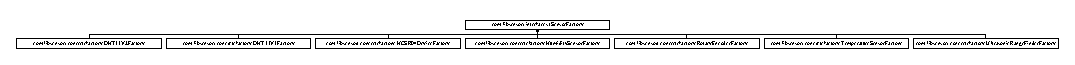
\includegraphics[height=0.430108cm]{interfacecom_1_1libsensorj_1_1interfaces_1_1ISensorFactory}
\end{center}
\end{figure}
\subsection*{Public Member Functions}
\begin{DoxyCompactItemize}
\item 
\hyperlink{interfacecom_1_1libsensorj_1_1interfaces_1_1ISensor}{I\+Sensor} \hyperlink{interfacecom_1_1libsensorj_1_1interfaces_1_1ISensorFactory_ac14c6d566c37c6a79c6db1e85634f25d}{create\+Sensor} ()
\item 
\hyperlink{classcom_1_1libsensorj_1_1interfaces_1_1IEvent}{I\+Event} \hyperlink{interfacecom_1_1libsensorj_1_1interfaces_1_1ISensorFactory_a2b074d01287a4e64677097255ba9e768}{create\+Event} ()
\end{DoxyCompactItemize}


\subsection{Detailed Description}
A factory for creating \hyperlink{interfacecom_1_1libsensorj_1_1interfaces_1_1ISensor}{I\+Sensor} objects. 

\subsection{Member Function Documentation}
\hypertarget{interfacecom_1_1libsensorj_1_1interfaces_1_1ISensorFactory_a2b074d01287a4e64677097255ba9e768}{}\index{com\+::libsensorj\+::interfaces\+::\+I\+Sensor\+Factory@{com\+::libsensorj\+::interfaces\+::\+I\+Sensor\+Factory}!create\+Event@{create\+Event}}
\index{create\+Event@{create\+Event}!com\+::libsensorj\+::interfaces\+::\+I\+Sensor\+Factory@{com\+::libsensorj\+::interfaces\+::\+I\+Sensor\+Factory}}
\subsubsection[{create\+Event}]{\setlength{\rightskip}{0pt plus 5cm}{\bf I\+Event} com.\+libsensorj.\+interfaces.\+I\+Sensor\+Factory.\+create\+Event (
\begin{DoxyParamCaption}
{}
\end{DoxyParamCaption}
)}\label{interfacecom_1_1libsensorj_1_1interfaces_1_1ISensorFactory_a2b074d01287a4e64677097255ba9e768}
Creates a new \hyperlink{classcom_1_1libsensorj_1_1interfaces_1_1IEvent}{I\+Event} object.

\begin{DoxyReturn}{Returns}
the \hyperlink{classcom_1_1libsensorj_1_1interfaces_1_1IEvent}{I\+Event} 
\end{DoxyReturn}


Implemented in \hyperlink{classcom_1_1libsensorj_1_1concretefactory_1_1DHT11V2Factory_a0eb0b480f4133c3eeb2728bd0fa45c58}{com.\+libsensorj.\+concretefactory.\+D\+H\+T11\+V2\+Factory}, \hyperlink{classcom_1_1libsensorj_1_1concretefactory_1_1TemperatureSensorFactory_adb3d5716b5e55f4fc037c0a95ec99688}{com.\+libsensorj.\+concretefactory.\+Temperature\+Sensor\+Factory}, \hyperlink{classcom_1_1libsensorj_1_1concretefactory_1_1HumiditySensorFactory_a43835bfa4c60faf39dfe64f67322b9e4}{com.\+libsensorj.\+concretefactory.\+Humidity\+Sensor\+Factory}, \hyperlink{classcom_1_1libsensorj_1_1concretefactory_1_1DHT11V3Factory_a7621f6dc5c877e6dfb160f68e50fd319}{com.\+libsensorj.\+concretefactory.\+D\+H\+T11\+V3\+Factory}, \hyperlink{classcom_1_1libsensorj_1_1concretefactory_1_1HCSR04DeviceFactory_aea88b0202d3021c4e55bd9cbf64da906}{com.\+libsensorj.\+concretefactory.\+H\+C\+S\+R04\+Device\+Factory}, \hyperlink{classcom_1_1libsensorj_1_1concretefactory_1_1UltrasonicRangeFinderFactory_a8a7d0c55346f1ab5630a878f6a3175fd}{com.\+libsensorj.\+concretefactory.\+Ultrasonic\+Range\+Finder\+Factory}, and \hyperlink{classcom_1_1libsensorj_1_1concretefactory_1_1RotaryEncoderFactory_a8f36c2cbdddcd1c71d438efafc73ffc2}{com.\+libsensorj.\+concretefactory.\+Rotary\+Encoder\+Factory}.

\hypertarget{interfacecom_1_1libsensorj_1_1interfaces_1_1ISensorFactory_ac14c6d566c37c6a79c6db1e85634f25d}{}\index{com\+::libsensorj\+::interfaces\+::\+I\+Sensor\+Factory@{com\+::libsensorj\+::interfaces\+::\+I\+Sensor\+Factory}!create\+Sensor@{create\+Sensor}}
\index{create\+Sensor@{create\+Sensor}!com\+::libsensorj\+::interfaces\+::\+I\+Sensor\+Factory@{com\+::libsensorj\+::interfaces\+::\+I\+Sensor\+Factory}}
\subsubsection[{create\+Sensor}]{\setlength{\rightskip}{0pt plus 5cm}{\bf I\+Sensor} com.\+libsensorj.\+interfaces.\+I\+Sensor\+Factory.\+create\+Sensor (
\begin{DoxyParamCaption}
{}
\end{DoxyParamCaption}
)}\label{interfacecom_1_1libsensorj_1_1interfaces_1_1ISensorFactory_ac14c6d566c37c6a79c6db1e85634f25d}
Creates a new \hyperlink{interfacecom_1_1libsensorj_1_1interfaces_1_1ISensor}{I\+Sensor} object.

\begin{DoxyReturn}{Returns}
the \hyperlink{interfacecom_1_1libsensorj_1_1interfaces_1_1ISensor}{I\+Sensor} 
\end{DoxyReturn}


Implemented in \hyperlink{classcom_1_1libsensorj_1_1concretefactory_1_1DHT11V2Factory_ac04eaebc748d420eb035439dfc1d2202}{com.\+libsensorj.\+concretefactory.\+D\+H\+T11\+V2\+Factory}, \hyperlink{classcom_1_1libsensorj_1_1concretefactory_1_1DHT11V3Factory_ad89c967025d654490729d2f69438805e}{com.\+libsensorj.\+concretefactory.\+D\+H\+T11\+V3\+Factory}, \hyperlink{classcom_1_1libsensorj_1_1concretefactory_1_1HCSR04DeviceFactory_a3d5c07b9ce458a3f56cfe5e7470b51df}{com.\+libsensorj.\+concretefactory.\+H\+C\+S\+R04\+Device\+Factory}, \hyperlink{classcom_1_1libsensorj_1_1concretefactory_1_1HumiditySensorFactory_aec6f80bd08e69d69ea6187067d11d28c}{com.\+libsensorj.\+concretefactory.\+Humidity\+Sensor\+Factory}, \hyperlink{classcom_1_1libsensorj_1_1concretefactory_1_1TemperatureSensorFactory_aeba8598ebe5c182154f63e0c94abdd70}{com.\+libsensorj.\+concretefactory.\+Temperature\+Sensor\+Factory}, \hyperlink{classcom_1_1libsensorj_1_1concretefactory_1_1UltrasonicRangeFinderFactory_a3aa6e46ef47bf97355df4d5cfb1b1e01}{com.\+libsensorj.\+concretefactory.\+Ultrasonic\+Range\+Finder\+Factory}, and \hyperlink{classcom_1_1libsensorj_1_1concretefactory_1_1RotaryEncoderFactory_a5f9c404d9b61d8aaf63cad82b87becd7}{com.\+libsensorj.\+concretefactory.\+Rotary\+Encoder\+Factory}.



The documentation for this interface was generated from the following file\+:\begin{DoxyCompactItemize}
\item 
main/java/com/libsensorj/interfaces/\hyperlink{ISensorFactory_8java}{I\+Sensor\+Factory.\+java}\end{DoxyCompactItemize}

\hypertarget{classcom_1_1libsensorj_1_1utils_1_1LibPins}{}\section{com.\+libsensorj.\+utils.\+Lib\+Pins Class Reference}
\label{classcom_1_1libsensorj_1_1utils_1_1LibPins}\index{com.\+libsensorj.\+utils.\+Lib\+Pins@{com.\+libsensorj.\+utils.\+Lib\+Pins}}
\subsection*{Static Public Member Functions}
\begin{DoxyCompactItemize}
\item 
static Pin \hyperlink{classcom_1_1libsensorj_1_1utils_1_1LibPins_ad30688404fa1f82b0ef038bc967255c3}{get\+Pin} (int pin\+Number)
\end{DoxyCompactItemize}
\subsection*{Static Package Functions}
\begin{DoxyCompactItemize}
\item 
\hyperlink{classcom_1_1libsensorj_1_1utils_1_1LibPins_a219d56076453e22e5971cfaaf50c70b1}{\mbox{[}static initializer\mbox{]}}
\end{DoxyCompactItemize}
\subsection*{Static Private Attributes}
\begin{DoxyCompactItemize}
\item 
static Map$<$ Integer, Pin $>$ \hyperlink{classcom_1_1libsensorj_1_1utils_1_1LibPins_a46bbd1e6636d9dc4f95d65a38ef33d5d}{gpio\+Pins}
\end{DoxyCompactItemize}


\subsection{Detailed Description}
The Class \hyperlink{classcom_1_1libsensorj_1_1utils_1_1LibPins}{Lib\+Pins}. 

\subsection{Member Function Documentation}
\hypertarget{classcom_1_1libsensorj_1_1utils_1_1LibPins_a219d56076453e22e5971cfaaf50c70b1}{}\index{com\+::libsensorj\+::utils\+::\+Lib\+Pins@{com\+::libsensorj\+::utils\+::\+Lib\+Pins}!\mbox{[}static initializer\mbox{]}@{[static initializer]}}
\index{\mbox{[}static initializer\mbox{]}@{[static initializer]}!com\+::libsensorj\+::utils\+::\+Lib\+Pins@{com\+::libsensorj\+::utils\+::\+Lib\+Pins}}
\subsubsection[{[static initializer]}]{\setlength{\rightskip}{0pt plus 5cm}com.\+libsensorj.\+utils.\+Lib\+Pins.\mbox{[}static initializer\mbox{]} (
\begin{DoxyParamCaption}
{}
\end{DoxyParamCaption}
)\hspace{0.3cm}{\ttfamily [static]}, {\ttfamily [package]}}\label{classcom_1_1libsensorj_1_1utils_1_1LibPins_a219d56076453e22e5971cfaaf50c70b1}
\hypertarget{classcom_1_1libsensorj_1_1utils_1_1LibPins_ad30688404fa1f82b0ef038bc967255c3}{}\index{com\+::libsensorj\+::utils\+::\+Lib\+Pins@{com\+::libsensorj\+::utils\+::\+Lib\+Pins}!get\+Pin@{get\+Pin}}
\index{get\+Pin@{get\+Pin}!com\+::libsensorj\+::utils\+::\+Lib\+Pins@{com\+::libsensorj\+::utils\+::\+Lib\+Pins}}
\subsubsection[{get\+Pin}]{\setlength{\rightskip}{0pt plus 5cm}static Pin com.\+libsensorj.\+utils.\+Lib\+Pins.\+get\+Pin (
\begin{DoxyParamCaption}
\item[{int}]{pin\+Number}
\end{DoxyParamCaption}
)\hspace{0.3cm}{\ttfamily [static]}}\label{classcom_1_1libsensorj_1_1utils_1_1LibPins_ad30688404fa1f82b0ef038bc967255c3}
Gets the pin.


\begin{DoxyParams}{Parameters}
{\em pin\+Number} & the pin number \\
\hline
\end{DoxyParams}
\begin{DoxyReturn}{Returns}
the pin 
\end{DoxyReturn}


\subsection{Member Data Documentation}
\hypertarget{classcom_1_1libsensorj_1_1utils_1_1LibPins_a46bbd1e6636d9dc4f95d65a38ef33d5d}{}\index{com\+::libsensorj\+::utils\+::\+Lib\+Pins@{com\+::libsensorj\+::utils\+::\+Lib\+Pins}!gpio\+Pins@{gpio\+Pins}}
\index{gpio\+Pins@{gpio\+Pins}!com\+::libsensorj\+::utils\+::\+Lib\+Pins@{com\+::libsensorj\+::utils\+::\+Lib\+Pins}}
\subsubsection[{gpio\+Pins}]{\setlength{\rightskip}{0pt plus 5cm}Map$<$Integer, Pin$>$ com.\+libsensorj.\+utils.\+Lib\+Pins.\+gpio\+Pins\hspace{0.3cm}{\ttfamily [static]}, {\ttfamily [private]}}\label{classcom_1_1libsensorj_1_1utils_1_1LibPins_a46bbd1e6636d9dc4f95d65a38ef33d5d}
The gpio pins. 

The documentation for this class was generated from the following file\+:\begin{DoxyCompactItemize}
\item 
main/java/com/libsensorj/utils/\hyperlink{LibPins_8java}{Lib\+Pins.\+java}\end{DoxyCompactItemize}

\hypertarget{classcom_1_1pi4j_1_1examples_1_1MyExample}{}\section{com.\+pi4j.\+examples.\+My\+Example Class Reference}
\label{classcom_1_1pi4j_1_1examples_1_1MyExample}\index{com.\+pi4j.\+examples.\+My\+Example@{com.\+pi4j.\+examples.\+My\+Example}}
\subsection*{Static Public Member Functions}
\begin{DoxyCompactItemize}
\item 
static void \hyperlink{classcom_1_1pi4j_1_1examples_1_1MyExample_a535756901ce4a1b547faf38117a3ec6f}{main} (String\mbox{[}$\,$\mbox{]} args)
\end{DoxyCompactItemize}


\subsection{Detailed Description}
The Class \hyperlink{classcom_1_1pi4j_1_1examples_1_1MyExample}{My\+Example}. 

\subsection{Member Function Documentation}
\hypertarget{classcom_1_1pi4j_1_1examples_1_1MyExample_a535756901ce4a1b547faf38117a3ec6f}{}\index{com\+::pi4j\+::examples\+::\+My\+Example@{com\+::pi4j\+::examples\+::\+My\+Example}!main@{main}}
\index{main@{main}!com\+::pi4j\+::examples\+::\+My\+Example@{com\+::pi4j\+::examples\+::\+My\+Example}}
\subsubsection[{main}]{\setlength{\rightskip}{0pt plus 5cm}static void com.\+pi4j.\+examples.\+My\+Example.\+main (
\begin{DoxyParamCaption}
\item[{String\mbox{[}$\,$\mbox{]}}]{args}
\end{DoxyParamCaption}
)\hspace{0.3cm}{\ttfamily [static]}}\label{classcom_1_1pi4j_1_1examples_1_1MyExample_a535756901ce4a1b547faf38117a3ec6f}
The main method.


\begin{DoxyParams}{Parameters}
{\em args} & the arguments \\
\hline
\end{DoxyParams}


The documentation for this class was generated from the following file\+:\begin{DoxyCompactItemize}
\item 
main/java/com/pi4j/examples/\hyperlink{MyExample_8java}{My\+Example.\+java}\end{DoxyCompactItemize}

\hypertarget{classcom_1_1libsensorj_1_1model_1_1Observer}{}\section{com.\+libsensorj.\+model.\+Observer Class Reference}
\label{classcom_1_1libsensorj_1_1model_1_1Observer}\index{com.\+libsensorj.\+model.\+Observer@{com.\+libsensorj.\+model.\+Observer}}
\subsection*{Public Member Functions}
\begin{DoxyCompactItemize}
\item 
\hyperlink{classcom_1_1libsensorj_1_1model_1_1Observer_a477725e32a58d3a8762d404799ec0161}{Observer} ()
\item 
\hyperlink{classcom_1_1libsensorj_1_1model_1_1Observer_a4933adee4c8da771eaa94415f6f840a7}{Observer} (String \hyperlink{classcom_1_1libsensorj_1_1model_1_1Observer_aa1f9da7634c35f34d5f20d5bc1562428}{observer\+Name})
\item 
String \hyperlink{classcom_1_1libsensorj_1_1model_1_1Observer_a8b873b9c90ad7f1ed055ea6713e0062a}{get\+Observer\+Name} ()
\item 
void \hyperlink{classcom_1_1libsensorj_1_1model_1_1Observer_a42628ca2b4d99e0df9fe1d70fec811b2}{set\+Observer\+Name} (String \hyperlink{classcom_1_1libsensorj_1_1model_1_1Observer_aa1f9da7634c35f34d5f20d5bc1562428}{observer\+Name})
\end{DoxyCompactItemize}
\subsection*{Private Attributes}
\begin{DoxyCompactItemize}
\item 
String \hyperlink{classcom_1_1libsensorj_1_1model_1_1Observer_aa1f9da7634c35f34d5f20d5bc1562428}{observer\+Name}
\end{DoxyCompactItemize}


\subsection{Detailed Description}
The Class \hyperlink{classcom_1_1libsensorj_1_1model_1_1Observer}{Observer}. 

\subsection{Constructor \& Destructor Documentation}
\hypertarget{classcom_1_1libsensorj_1_1model_1_1Observer_a477725e32a58d3a8762d404799ec0161}{}\index{com\+::libsensorj\+::model\+::\+Observer@{com\+::libsensorj\+::model\+::\+Observer}!Observer@{Observer}}
\index{Observer@{Observer}!com\+::libsensorj\+::model\+::\+Observer@{com\+::libsensorj\+::model\+::\+Observer}}
\subsubsection[{Observer}]{\setlength{\rightskip}{0pt plus 5cm}com.\+libsensorj.\+model.\+Observer.\+Observer (
\begin{DoxyParamCaption}
{}
\end{DoxyParamCaption}
)}\label{classcom_1_1libsensorj_1_1model_1_1Observer_a477725e32a58d3a8762d404799ec0161}
Instantiates a new observer. \hypertarget{classcom_1_1libsensorj_1_1model_1_1Observer_a4933adee4c8da771eaa94415f6f840a7}{}\index{com\+::libsensorj\+::model\+::\+Observer@{com\+::libsensorj\+::model\+::\+Observer}!Observer@{Observer}}
\index{Observer@{Observer}!com\+::libsensorj\+::model\+::\+Observer@{com\+::libsensorj\+::model\+::\+Observer}}
\subsubsection[{Observer}]{\setlength{\rightskip}{0pt plus 5cm}com.\+libsensorj.\+model.\+Observer.\+Observer (
\begin{DoxyParamCaption}
\item[{String}]{observer\+Name}
\end{DoxyParamCaption}
)}\label{classcom_1_1libsensorj_1_1model_1_1Observer_a4933adee4c8da771eaa94415f6f840a7}
Instantiates a new observer.


\begin{DoxyParams}{Parameters}
{\em observer\+Name} & the observer name \\
\hline
\end{DoxyParams}


\subsection{Member Function Documentation}
\hypertarget{classcom_1_1libsensorj_1_1model_1_1Observer_a8b873b9c90ad7f1ed055ea6713e0062a}{}\index{com\+::libsensorj\+::model\+::\+Observer@{com\+::libsensorj\+::model\+::\+Observer}!get\+Observer\+Name@{get\+Observer\+Name}}
\index{get\+Observer\+Name@{get\+Observer\+Name}!com\+::libsensorj\+::model\+::\+Observer@{com\+::libsensorj\+::model\+::\+Observer}}
\subsubsection[{get\+Observer\+Name}]{\setlength{\rightskip}{0pt plus 5cm}String com.\+libsensorj.\+model.\+Observer.\+get\+Observer\+Name (
\begin{DoxyParamCaption}
{}
\end{DoxyParamCaption}
)}\label{classcom_1_1libsensorj_1_1model_1_1Observer_a8b873b9c90ad7f1ed055ea6713e0062a}
Gets the observer name.

\begin{DoxyReturn}{Returns}
the observer name 
\end{DoxyReturn}
\hypertarget{classcom_1_1libsensorj_1_1model_1_1Observer_a42628ca2b4d99e0df9fe1d70fec811b2}{}\index{com\+::libsensorj\+::model\+::\+Observer@{com\+::libsensorj\+::model\+::\+Observer}!set\+Observer\+Name@{set\+Observer\+Name}}
\index{set\+Observer\+Name@{set\+Observer\+Name}!com\+::libsensorj\+::model\+::\+Observer@{com\+::libsensorj\+::model\+::\+Observer}}
\subsubsection[{set\+Observer\+Name}]{\setlength{\rightskip}{0pt plus 5cm}void com.\+libsensorj.\+model.\+Observer.\+set\+Observer\+Name (
\begin{DoxyParamCaption}
\item[{String}]{observer\+Name}
\end{DoxyParamCaption}
)}\label{classcom_1_1libsensorj_1_1model_1_1Observer_a42628ca2b4d99e0df9fe1d70fec811b2}
Sets the observer name.


\begin{DoxyParams}{Parameters}
{\em observer\+Name} & the new observer name \\
\hline
\end{DoxyParams}


\subsection{Member Data Documentation}
\hypertarget{classcom_1_1libsensorj_1_1model_1_1Observer_aa1f9da7634c35f34d5f20d5bc1562428}{}\index{com\+::libsensorj\+::model\+::\+Observer@{com\+::libsensorj\+::model\+::\+Observer}!observer\+Name@{observer\+Name}}
\index{observer\+Name@{observer\+Name}!com\+::libsensorj\+::model\+::\+Observer@{com\+::libsensorj\+::model\+::\+Observer}}
\subsubsection[{observer\+Name}]{\setlength{\rightskip}{0pt plus 5cm}String com.\+libsensorj.\+model.\+Observer.\+observer\+Name\hspace{0.3cm}{\ttfamily [private]}}\label{classcom_1_1libsensorj_1_1model_1_1Observer_aa1f9da7634c35f34d5f20d5bc1562428}
The observer name. 

The documentation for this class was generated from the following file\+:\begin{DoxyCompactItemize}
\item 
main/java/com/libsensorj/model/\hyperlink{Observer_8java}{Observer.\+java}\end{DoxyCompactItemize}

\hypertarget{enumcom_1_1libsensorj_1_1utils_1_1PinNumbers}{}\section{com.\+libsensorj.\+utils.\+Pin\+Numbers Enum Reference}
\label{enumcom_1_1libsensorj_1_1utils_1_1PinNumbers}\index{com.\+libsensorj.\+utils.\+Pin\+Numbers@{com.\+libsensorj.\+utils.\+Pin\+Numbers}}
\subsection*{Public Member Functions}
\begin{DoxyCompactItemize}
\item 
\hyperlink{enumcom_1_1libsensorj_1_1utils_1_1PinNumbers_a968a61df9cb0d58d376afe58c0e819a1}{Pin\+Numbers} (Pin pin)
\end{DoxyCompactItemize}
\subsection*{Public Attributes}
\begin{DoxyCompactItemize}
\item 
\hyperlink{enumcom_1_1libsensorj_1_1utils_1_1PinNumbers_a3ef0e0eade17450513e7722a45850223}{P\+I\+N\+\_\+00} =(Raspi\+Pin.\+G\+P\+I\+O\+\_\+00)
\item 
\hyperlink{enumcom_1_1libsensorj_1_1utils_1_1PinNumbers_a685c54b4b889232a644256053628b751}{P\+I\+N\+\_\+01} =(Raspi\+Pin.\+G\+P\+I\+O\+\_\+01)
\item 
\hyperlink{enumcom_1_1libsensorj_1_1utils_1_1PinNumbers_afb610737394f458dff87b1df785b75ea}{P\+I\+N\+\_\+02} =(Raspi\+Pin.\+G\+P\+I\+O\+\_\+02)
\item 
\hyperlink{enumcom_1_1libsensorj_1_1utils_1_1PinNumbers_a1bc2b6b45afefca090b810e9f8acbb27}{P\+I\+N\+\_\+03} =(Raspi\+Pin.\+G\+P\+I\+O\+\_\+03)
\item 
\hyperlink{enumcom_1_1libsensorj_1_1utils_1_1PinNumbers_a93afd56e9549da0c1d58a541be66bd3e}{P\+I\+N\+\_\+04} =(Raspi\+Pin.\+G\+P\+I\+O\+\_\+04)
\item 
\hyperlink{enumcom_1_1libsensorj_1_1utils_1_1PinNumbers_ae8da4fe40f2c19e201f9bfc201144c5a}{P\+I\+N\+\_\+05} =(Raspi\+Pin.\+G\+P\+I\+O\+\_\+05)
\item 
\hyperlink{enumcom_1_1libsensorj_1_1utils_1_1PinNumbers_a04c882940fbe6fa70f06f533f0693e5d}{P\+I\+N\+\_\+06} =(Raspi\+Pin.\+G\+P\+I\+O\+\_\+06)
\item 
\hyperlink{enumcom_1_1libsensorj_1_1utils_1_1PinNumbers_ab8b7352afed72c8b1ea2c55d9050b99b}{P\+I\+N\+\_\+07} =(Raspi\+Pin.\+G\+P\+I\+O\+\_\+07)
\item 
\hyperlink{enumcom_1_1libsensorj_1_1utils_1_1PinNumbers_a9d3ead7c0ee9cc96ab2b4f2519c3e4e4}{P\+I\+N\+\_\+08} =(Raspi\+Pin.\+G\+P\+I\+O\+\_\+08)
\item 
\hyperlink{enumcom_1_1libsensorj_1_1utils_1_1PinNumbers_a054eb5753d44984377ca36b6bd790543}{P\+I\+N\+\_\+09} =(Raspi\+Pin.\+G\+P\+I\+O\+\_\+09)
\item 
\hyperlink{enumcom_1_1libsensorj_1_1utils_1_1PinNumbers_a239afb6f67b7e2515ba8cba38c139f25}{P\+I\+N\+\_\+10} =(Raspi\+Pin.\+G\+P\+I\+O\+\_\+10)
\item 
\hyperlink{enumcom_1_1libsensorj_1_1utils_1_1PinNumbers_a5ee3dd0f90eb66a8594ad89a2a0470eb}{P\+I\+N\+\_\+11} =(Raspi\+Pin.\+G\+P\+I\+O\+\_\+11)
\item 
\hyperlink{enumcom_1_1libsensorj_1_1utils_1_1PinNumbers_ae19026133ddb5e75c9778599fcb803fe}{P\+I\+N\+\_\+12} =(Raspi\+Pin.\+G\+P\+I\+O\+\_\+12)
\item 
\hyperlink{enumcom_1_1libsensorj_1_1utils_1_1PinNumbers_a5e893c4d5093998d44431b35b7b9ba7c}{P\+I\+N\+\_\+13} =(Raspi\+Pin.\+G\+P\+I\+O\+\_\+13)
\item 
\hyperlink{enumcom_1_1libsensorj_1_1utils_1_1PinNumbers_ac1c99a7202d314de7d9f4a772c55a0ca}{P\+I\+N\+\_\+14} =(Raspi\+Pin.\+G\+P\+I\+O\+\_\+14)
\item 
\hyperlink{enumcom_1_1libsensorj_1_1utils_1_1PinNumbers_a1e89f76fc2c08c4929b36ab869e4c879}{P\+I\+N\+\_\+15} =(Raspi\+Pin.\+G\+P\+I\+O\+\_\+15)
\item 
\hyperlink{enumcom_1_1libsensorj_1_1utils_1_1PinNumbers_a1ffacc29c4eda74be0327a9acd772a1a}{P\+I\+N\+\_\+16} =(Raspi\+Pin.\+G\+P\+I\+O\+\_\+16)
\item 
\hyperlink{enumcom_1_1libsensorj_1_1utils_1_1PinNumbers_a6d060a58a23f8f9ab2af2b3787919db5}{P\+I\+N\+\_\+17} =(Raspi\+Pin.\+G\+P\+I\+O\+\_\+17)
\item 
\hyperlink{enumcom_1_1libsensorj_1_1utils_1_1PinNumbers_ac6d1e80afe2e16591fa1de746930670a}{P\+I\+N\+\_\+18} =(Raspi\+Pin.\+G\+P\+I\+O\+\_\+18)
\item 
\hyperlink{enumcom_1_1libsensorj_1_1utils_1_1PinNumbers_a4443c323b9599c9f323734c354bf4b03}{P\+I\+N\+\_\+19} =(Raspi\+Pin.\+G\+P\+I\+O\+\_\+19)
\item 
\hyperlink{enumcom_1_1libsensorj_1_1utils_1_1PinNumbers_a7382cd6abefb7891a990e1e4919923da}{P\+I\+N\+\_\+20} =(Raspi\+Pin.\+G\+P\+I\+O\+\_\+20)
\item 
\hyperlink{enumcom_1_1libsensorj_1_1utils_1_1PinNumbers_a53700cbc79faf1650f0f46862458a524}{P\+I\+N\+\_\+21} =(Raspi\+Pin.\+G\+P\+I\+O\+\_\+21)
\item 
\hyperlink{enumcom_1_1libsensorj_1_1utils_1_1PinNumbers_a136ce66a6474359af2728ac7bf4b81db}{P\+I\+N\+\_\+22} =(Raspi\+Pin.\+G\+P\+I\+O\+\_\+22)
\item 
\hyperlink{enumcom_1_1libsensorj_1_1utils_1_1PinNumbers_a5c12880fb3fca2bfede5782df98de3bb}{P\+I\+N\+\_\+23} =(Raspi\+Pin.\+G\+P\+I\+O\+\_\+23)
\item 
\hyperlink{enumcom_1_1libsensorj_1_1utils_1_1PinNumbers_a8d54d3af55e1b5460f88d7faa218e545}{P\+I\+N\+\_\+24} =(Raspi\+Pin.\+G\+P\+I\+O\+\_\+24)
\item 
\hyperlink{enumcom_1_1libsensorj_1_1utils_1_1PinNumbers_a64907a187e76e03b5071d26b42bc8ff7}{P\+I\+N\+\_\+25} =(Raspi\+Pin.\+G\+P\+I\+O\+\_\+25)
\item 
\hyperlink{enumcom_1_1libsensorj_1_1utils_1_1PinNumbers_a66592f4af694df2ec1605d26f3b9f458}{P\+I\+N\+\_\+26} =(Raspi\+Pin.\+G\+P\+I\+O\+\_\+26)
\item 
\hyperlink{enumcom_1_1libsensorj_1_1utils_1_1PinNumbers_ac5368fe64b7b6003c89065bea9e7ca49}{P\+I\+N\+\_\+27} =(Raspi\+Pin.\+G\+P\+I\+O\+\_\+27)
\item 
\hyperlink{enumcom_1_1libsensorj_1_1utils_1_1PinNumbers_af7bec7611fed7e9b64e25485f2378f81}{P\+I\+N\+\_\+28} =(Raspi\+Pin.\+G\+P\+I\+O\+\_\+28)
\item 
\hyperlink{enumcom_1_1libsensorj_1_1utils_1_1PinNumbers_a78cc24e6c72e7dceb4a9a152cc9da41f}{P\+I\+N\+\_\+29} =(Raspi\+Pin.\+G\+P\+I\+O\+\_\+29)
\item 
Pin \hyperlink{enumcom_1_1libsensorj_1_1utils_1_1PinNumbers_a82cad4bc9bde38b8b6e9f33f5ce8bf3d}{pin\+Number}
\end{DoxyCompactItemize}


\subsection{Detailed Description}
The Enum \hyperlink{enumcom_1_1libsensorj_1_1utils_1_1PinNumbers}{Pin\+Numbers}. 

\subsection{Constructor \& Destructor Documentation}
\hypertarget{enumcom_1_1libsensorj_1_1utils_1_1PinNumbers_a968a61df9cb0d58d376afe58c0e819a1}{}\index{com\+::libsensorj\+::utils\+::\+Pin\+Numbers@{com\+::libsensorj\+::utils\+::\+Pin\+Numbers}!Pin\+Numbers@{Pin\+Numbers}}
\index{Pin\+Numbers@{Pin\+Numbers}!com\+::libsensorj\+::utils\+::\+Pin\+Numbers@{com\+::libsensorj\+::utils\+::\+Pin\+Numbers}}
\subsubsection[{Pin\+Numbers}]{\setlength{\rightskip}{0pt plus 5cm}com.\+libsensorj.\+utils.\+Pin\+Numbers.\+Pin\+Numbers (
\begin{DoxyParamCaption}
\item[{Pin}]{pin}
\end{DoxyParamCaption}
)}\label{enumcom_1_1libsensorj_1_1utils_1_1PinNumbers_a968a61df9cb0d58d376afe58c0e819a1}
Instantiates new pin numbers.


\begin{DoxyParams}{Parameters}
{\em pin} & the pin \\
\hline
\end{DoxyParams}


\subsection{Member Data Documentation}
\hypertarget{enumcom_1_1libsensorj_1_1utils_1_1PinNumbers_a3ef0e0eade17450513e7722a45850223}{}\index{com\+::libsensorj\+::utils\+::\+Pin\+Numbers@{com\+::libsensorj\+::utils\+::\+Pin\+Numbers}!P\+I\+N\+\_\+00@{P\+I\+N\+\_\+00}}
\index{P\+I\+N\+\_\+00@{P\+I\+N\+\_\+00}!com\+::libsensorj\+::utils\+::\+Pin\+Numbers@{com\+::libsensorj\+::utils\+::\+Pin\+Numbers}}
\subsubsection[{P\+I\+N\+\_\+00}]{\setlength{\rightskip}{0pt plus 5cm}com.\+libsensorj.\+utils.\+Pin\+Numbers.\+P\+I\+N\+\_\+00 =(Raspi\+Pin.\+G\+P\+I\+O\+\_\+00)}\label{enumcom_1_1libsensorj_1_1utils_1_1PinNumbers_a3ef0e0eade17450513e7722a45850223}
The P\+I n\+\_\+00. \hypertarget{enumcom_1_1libsensorj_1_1utils_1_1PinNumbers_a685c54b4b889232a644256053628b751}{}\index{com\+::libsensorj\+::utils\+::\+Pin\+Numbers@{com\+::libsensorj\+::utils\+::\+Pin\+Numbers}!P\+I\+N\+\_\+01@{P\+I\+N\+\_\+01}}
\index{P\+I\+N\+\_\+01@{P\+I\+N\+\_\+01}!com\+::libsensorj\+::utils\+::\+Pin\+Numbers@{com\+::libsensorj\+::utils\+::\+Pin\+Numbers}}
\subsubsection[{P\+I\+N\+\_\+01}]{\setlength{\rightskip}{0pt plus 5cm}com.\+libsensorj.\+utils.\+Pin\+Numbers.\+P\+I\+N\+\_\+01 =(Raspi\+Pin.\+G\+P\+I\+O\+\_\+01)}\label{enumcom_1_1libsensorj_1_1utils_1_1PinNumbers_a685c54b4b889232a644256053628b751}
The P\+I n\+\_\+01. \hypertarget{enumcom_1_1libsensorj_1_1utils_1_1PinNumbers_afb610737394f458dff87b1df785b75ea}{}\index{com\+::libsensorj\+::utils\+::\+Pin\+Numbers@{com\+::libsensorj\+::utils\+::\+Pin\+Numbers}!P\+I\+N\+\_\+02@{P\+I\+N\+\_\+02}}
\index{P\+I\+N\+\_\+02@{P\+I\+N\+\_\+02}!com\+::libsensorj\+::utils\+::\+Pin\+Numbers@{com\+::libsensorj\+::utils\+::\+Pin\+Numbers}}
\subsubsection[{P\+I\+N\+\_\+02}]{\setlength{\rightskip}{0pt plus 5cm}com.\+libsensorj.\+utils.\+Pin\+Numbers.\+P\+I\+N\+\_\+02 =(Raspi\+Pin.\+G\+P\+I\+O\+\_\+02)}\label{enumcom_1_1libsensorj_1_1utils_1_1PinNumbers_afb610737394f458dff87b1df785b75ea}
The P\+I n\+\_\+02. \hypertarget{enumcom_1_1libsensorj_1_1utils_1_1PinNumbers_a1bc2b6b45afefca090b810e9f8acbb27}{}\index{com\+::libsensorj\+::utils\+::\+Pin\+Numbers@{com\+::libsensorj\+::utils\+::\+Pin\+Numbers}!P\+I\+N\+\_\+03@{P\+I\+N\+\_\+03}}
\index{P\+I\+N\+\_\+03@{P\+I\+N\+\_\+03}!com\+::libsensorj\+::utils\+::\+Pin\+Numbers@{com\+::libsensorj\+::utils\+::\+Pin\+Numbers}}
\subsubsection[{P\+I\+N\+\_\+03}]{\setlength{\rightskip}{0pt plus 5cm}com.\+libsensorj.\+utils.\+Pin\+Numbers.\+P\+I\+N\+\_\+03 =(Raspi\+Pin.\+G\+P\+I\+O\+\_\+03)}\label{enumcom_1_1libsensorj_1_1utils_1_1PinNumbers_a1bc2b6b45afefca090b810e9f8acbb27}
The P\+I n\+\_\+03. \hypertarget{enumcom_1_1libsensorj_1_1utils_1_1PinNumbers_a93afd56e9549da0c1d58a541be66bd3e}{}\index{com\+::libsensorj\+::utils\+::\+Pin\+Numbers@{com\+::libsensorj\+::utils\+::\+Pin\+Numbers}!P\+I\+N\+\_\+04@{P\+I\+N\+\_\+04}}
\index{P\+I\+N\+\_\+04@{P\+I\+N\+\_\+04}!com\+::libsensorj\+::utils\+::\+Pin\+Numbers@{com\+::libsensorj\+::utils\+::\+Pin\+Numbers}}
\subsubsection[{P\+I\+N\+\_\+04}]{\setlength{\rightskip}{0pt plus 5cm}com.\+libsensorj.\+utils.\+Pin\+Numbers.\+P\+I\+N\+\_\+04 =(Raspi\+Pin.\+G\+P\+I\+O\+\_\+04)}\label{enumcom_1_1libsensorj_1_1utils_1_1PinNumbers_a93afd56e9549da0c1d58a541be66bd3e}
The P\+I n\+\_\+04. \hypertarget{enumcom_1_1libsensorj_1_1utils_1_1PinNumbers_ae8da4fe40f2c19e201f9bfc201144c5a}{}\index{com\+::libsensorj\+::utils\+::\+Pin\+Numbers@{com\+::libsensorj\+::utils\+::\+Pin\+Numbers}!P\+I\+N\+\_\+05@{P\+I\+N\+\_\+05}}
\index{P\+I\+N\+\_\+05@{P\+I\+N\+\_\+05}!com\+::libsensorj\+::utils\+::\+Pin\+Numbers@{com\+::libsensorj\+::utils\+::\+Pin\+Numbers}}
\subsubsection[{P\+I\+N\+\_\+05}]{\setlength{\rightskip}{0pt plus 5cm}com.\+libsensorj.\+utils.\+Pin\+Numbers.\+P\+I\+N\+\_\+05 =(Raspi\+Pin.\+G\+P\+I\+O\+\_\+05)}\label{enumcom_1_1libsensorj_1_1utils_1_1PinNumbers_ae8da4fe40f2c19e201f9bfc201144c5a}
The P\+I n\+\_\+05. \hypertarget{enumcom_1_1libsensorj_1_1utils_1_1PinNumbers_a04c882940fbe6fa70f06f533f0693e5d}{}\index{com\+::libsensorj\+::utils\+::\+Pin\+Numbers@{com\+::libsensorj\+::utils\+::\+Pin\+Numbers}!P\+I\+N\+\_\+06@{P\+I\+N\+\_\+06}}
\index{P\+I\+N\+\_\+06@{P\+I\+N\+\_\+06}!com\+::libsensorj\+::utils\+::\+Pin\+Numbers@{com\+::libsensorj\+::utils\+::\+Pin\+Numbers}}
\subsubsection[{P\+I\+N\+\_\+06}]{\setlength{\rightskip}{0pt plus 5cm}com.\+libsensorj.\+utils.\+Pin\+Numbers.\+P\+I\+N\+\_\+06 =(Raspi\+Pin.\+G\+P\+I\+O\+\_\+06)}\label{enumcom_1_1libsensorj_1_1utils_1_1PinNumbers_a04c882940fbe6fa70f06f533f0693e5d}
The P\+I n\+\_\+06. \hypertarget{enumcom_1_1libsensorj_1_1utils_1_1PinNumbers_ab8b7352afed72c8b1ea2c55d9050b99b}{}\index{com\+::libsensorj\+::utils\+::\+Pin\+Numbers@{com\+::libsensorj\+::utils\+::\+Pin\+Numbers}!P\+I\+N\+\_\+07@{P\+I\+N\+\_\+07}}
\index{P\+I\+N\+\_\+07@{P\+I\+N\+\_\+07}!com\+::libsensorj\+::utils\+::\+Pin\+Numbers@{com\+::libsensorj\+::utils\+::\+Pin\+Numbers}}
\subsubsection[{P\+I\+N\+\_\+07}]{\setlength{\rightskip}{0pt plus 5cm}com.\+libsensorj.\+utils.\+Pin\+Numbers.\+P\+I\+N\+\_\+07 =(Raspi\+Pin.\+G\+P\+I\+O\+\_\+07)}\label{enumcom_1_1libsensorj_1_1utils_1_1PinNumbers_ab8b7352afed72c8b1ea2c55d9050b99b}
The P\+I n\+\_\+07. \hypertarget{enumcom_1_1libsensorj_1_1utils_1_1PinNumbers_a9d3ead7c0ee9cc96ab2b4f2519c3e4e4}{}\index{com\+::libsensorj\+::utils\+::\+Pin\+Numbers@{com\+::libsensorj\+::utils\+::\+Pin\+Numbers}!P\+I\+N\+\_\+08@{P\+I\+N\+\_\+08}}
\index{P\+I\+N\+\_\+08@{P\+I\+N\+\_\+08}!com\+::libsensorj\+::utils\+::\+Pin\+Numbers@{com\+::libsensorj\+::utils\+::\+Pin\+Numbers}}
\subsubsection[{P\+I\+N\+\_\+08}]{\setlength{\rightskip}{0pt plus 5cm}com.\+libsensorj.\+utils.\+Pin\+Numbers.\+P\+I\+N\+\_\+08 =(Raspi\+Pin.\+G\+P\+I\+O\+\_\+08)}\label{enumcom_1_1libsensorj_1_1utils_1_1PinNumbers_a9d3ead7c0ee9cc96ab2b4f2519c3e4e4}
The P\+I n\+\_\+08. \hypertarget{enumcom_1_1libsensorj_1_1utils_1_1PinNumbers_a054eb5753d44984377ca36b6bd790543}{}\index{com\+::libsensorj\+::utils\+::\+Pin\+Numbers@{com\+::libsensorj\+::utils\+::\+Pin\+Numbers}!P\+I\+N\+\_\+09@{P\+I\+N\+\_\+09}}
\index{P\+I\+N\+\_\+09@{P\+I\+N\+\_\+09}!com\+::libsensorj\+::utils\+::\+Pin\+Numbers@{com\+::libsensorj\+::utils\+::\+Pin\+Numbers}}
\subsubsection[{P\+I\+N\+\_\+09}]{\setlength{\rightskip}{0pt plus 5cm}com.\+libsensorj.\+utils.\+Pin\+Numbers.\+P\+I\+N\+\_\+09 =(Raspi\+Pin.\+G\+P\+I\+O\+\_\+09)}\label{enumcom_1_1libsensorj_1_1utils_1_1PinNumbers_a054eb5753d44984377ca36b6bd790543}
The P\+I n\+\_\+09. \hypertarget{enumcom_1_1libsensorj_1_1utils_1_1PinNumbers_a239afb6f67b7e2515ba8cba38c139f25}{}\index{com\+::libsensorj\+::utils\+::\+Pin\+Numbers@{com\+::libsensorj\+::utils\+::\+Pin\+Numbers}!P\+I\+N\+\_\+10@{P\+I\+N\+\_\+10}}
\index{P\+I\+N\+\_\+10@{P\+I\+N\+\_\+10}!com\+::libsensorj\+::utils\+::\+Pin\+Numbers@{com\+::libsensorj\+::utils\+::\+Pin\+Numbers}}
\subsubsection[{P\+I\+N\+\_\+10}]{\setlength{\rightskip}{0pt plus 5cm}com.\+libsensorj.\+utils.\+Pin\+Numbers.\+P\+I\+N\+\_\+10 =(Raspi\+Pin.\+G\+P\+I\+O\+\_\+10)}\label{enumcom_1_1libsensorj_1_1utils_1_1PinNumbers_a239afb6f67b7e2515ba8cba38c139f25}
The P\+I n\+\_\+10. \hypertarget{enumcom_1_1libsensorj_1_1utils_1_1PinNumbers_a5ee3dd0f90eb66a8594ad89a2a0470eb}{}\index{com\+::libsensorj\+::utils\+::\+Pin\+Numbers@{com\+::libsensorj\+::utils\+::\+Pin\+Numbers}!P\+I\+N\+\_\+11@{P\+I\+N\+\_\+11}}
\index{P\+I\+N\+\_\+11@{P\+I\+N\+\_\+11}!com\+::libsensorj\+::utils\+::\+Pin\+Numbers@{com\+::libsensorj\+::utils\+::\+Pin\+Numbers}}
\subsubsection[{P\+I\+N\+\_\+11}]{\setlength{\rightskip}{0pt plus 5cm}com.\+libsensorj.\+utils.\+Pin\+Numbers.\+P\+I\+N\+\_\+11 =(Raspi\+Pin.\+G\+P\+I\+O\+\_\+11)}\label{enumcom_1_1libsensorj_1_1utils_1_1PinNumbers_a5ee3dd0f90eb66a8594ad89a2a0470eb}
The P\+I n\+\_\+11. \hypertarget{enumcom_1_1libsensorj_1_1utils_1_1PinNumbers_ae19026133ddb5e75c9778599fcb803fe}{}\index{com\+::libsensorj\+::utils\+::\+Pin\+Numbers@{com\+::libsensorj\+::utils\+::\+Pin\+Numbers}!P\+I\+N\+\_\+12@{P\+I\+N\+\_\+12}}
\index{P\+I\+N\+\_\+12@{P\+I\+N\+\_\+12}!com\+::libsensorj\+::utils\+::\+Pin\+Numbers@{com\+::libsensorj\+::utils\+::\+Pin\+Numbers}}
\subsubsection[{P\+I\+N\+\_\+12}]{\setlength{\rightskip}{0pt plus 5cm}com.\+libsensorj.\+utils.\+Pin\+Numbers.\+P\+I\+N\+\_\+12 =(Raspi\+Pin.\+G\+P\+I\+O\+\_\+12)}\label{enumcom_1_1libsensorj_1_1utils_1_1PinNumbers_ae19026133ddb5e75c9778599fcb803fe}
The P\+I n\+\_\+12. \hypertarget{enumcom_1_1libsensorj_1_1utils_1_1PinNumbers_a5e893c4d5093998d44431b35b7b9ba7c}{}\index{com\+::libsensorj\+::utils\+::\+Pin\+Numbers@{com\+::libsensorj\+::utils\+::\+Pin\+Numbers}!P\+I\+N\+\_\+13@{P\+I\+N\+\_\+13}}
\index{P\+I\+N\+\_\+13@{P\+I\+N\+\_\+13}!com\+::libsensorj\+::utils\+::\+Pin\+Numbers@{com\+::libsensorj\+::utils\+::\+Pin\+Numbers}}
\subsubsection[{P\+I\+N\+\_\+13}]{\setlength{\rightskip}{0pt plus 5cm}com.\+libsensorj.\+utils.\+Pin\+Numbers.\+P\+I\+N\+\_\+13 =(Raspi\+Pin.\+G\+P\+I\+O\+\_\+13)}\label{enumcom_1_1libsensorj_1_1utils_1_1PinNumbers_a5e893c4d5093998d44431b35b7b9ba7c}
The P\+I n\+\_\+13. \hypertarget{enumcom_1_1libsensorj_1_1utils_1_1PinNumbers_ac1c99a7202d314de7d9f4a772c55a0ca}{}\index{com\+::libsensorj\+::utils\+::\+Pin\+Numbers@{com\+::libsensorj\+::utils\+::\+Pin\+Numbers}!P\+I\+N\+\_\+14@{P\+I\+N\+\_\+14}}
\index{P\+I\+N\+\_\+14@{P\+I\+N\+\_\+14}!com\+::libsensorj\+::utils\+::\+Pin\+Numbers@{com\+::libsensorj\+::utils\+::\+Pin\+Numbers}}
\subsubsection[{P\+I\+N\+\_\+14}]{\setlength{\rightskip}{0pt plus 5cm}com.\+libsensorj.\+utils.\+Pin\+Numbers.\+P\+I\+N\+\_\+14 =(Raspi\+Pin.\+G\+P\+I\+O\+\_\+14)}\label{enumcom_1_1libsensorj_1_1utils_1_1PinNumbers_ac1c99a7202d314de7d9f4a772c55a0ca}
The P\+I n\+\_\+14. \hypertarget{enumcom_1_1libsensorj_1_1utils_1_1PinNumbers_a1e89f76fc2c08c4929b36ab869e4c879}{}\index{com\+::libsensorj\+::utils\+::\+Pin\+Numbers@{com\+::libsensorj\+::utils\+::\+Pin\+Numbers}!P\+I\+N\+\_\+15@{P\+I\+N\+\_\+15}}
\index{P\+I\+N\+\_\+15@{P\+I\+N\+\_\+15}!com\+::libsensorj\+::utils\+::\+Pin\+Numbers@{com\+::libsensorj\+::utils\+::\+Pin\+Numbers}}
\subsubsection[{P\+I\+N\+\_\+15}]{\setlength{\rightskip}{0pt plus 5cm}com.\+libsensorj.\+utils.\+Pin\+Numbers.\+P\+I\+N\+\_\+15 =(Raspi\+Pin.\+G\+P\+I\+O\+\_\+15)}\label{enumcom_1_1libsensorj_1_1utils_1_1PinNumbers_a1e89f76fc2c08c4929b36ab869e4c879}
The P\+I n\+\_\+15. \hypertarget{enumcom_1_1libsensorj_1_1utils_1_1PinNumbers_a1ffacc29c4eda74be0327a9acd772a1a}{}\index{com\+::libsensorj\+::utils\+::\+Pin\+Numbers@{com\+::libsensorj\+::utils\+::\+Pin\+Numbers}!P\+I\+N\+\_\+16@{P\+I\+N\+\_\+16}}
\index{P\+I\+N\+\_\+16@{P\+I\+N\+\_\+16}!com\+::libsensorj\+::utils\+::\+Pin\+Numbers@{com\+::libsensorj\+::utils\+::\+Pin\+Numbers}}
\subsubsection[{P\+I\+N\+\_\+16}]{\setlength{\rightskip}{0pt plus 5cm}com.\+libsensorj.\+utils.\+Pin\+Numbers.\+P\+I\+N\+\_\+16 =(Raspi\+Pin.\+G\+P\+I\+O\+\_\+16)}\label{enumcom_1_1libsensorj_1_1utils_1_1PinNumbers_a1ffacc29c4eda74be0327a9acd772a1a}
The P\+I n\+\_\+16. \hypertarget{enumcom_1_1libsensorj_1_1utils_1_1PinNumbers_a6d060a58a23f8f9ab2af2b3787919db5}{}\index{com\+::libsensorj\+::utils\+::\+Pin\+Numbers@{com\+::libsensorj\+::utils\+::\+Pin\+Numbers}!P\+I\+N\+\_\+17@{P\+I\+N\+\_\+17}}
\index{P\+I\+N\+\_\+17@{P\+I\+N\+\_\+17}!com\+::libsensorj\+::utils\+::\+Pin\+Numbers@{com\+::libsensorj\+::utils\+::\+Pin\+Numbers}}
\subsubsection[{P\+I\+N\+\_\+17}]{\setlength{\rightskip}{0pt plus 5cm}com.\+libsensorj.\+utils.\+Pin\+Numbers.\+P\+I\+N\+\_\+17 =(Raspi\+Pin.\+G\+P\+I\+O\+\_\+17)}\label{enumcom_1_1libsensorj_1_1utils_1_1PinNumbers_a6d060a58a23f8f9ab2af2b3787919db5}
The P\+I n\+\_\+17. \hypertarget{enumcom_1_1libsensorj_1_1utils_1_1PinNumbers_ac6d1e80afe2e16591fa1de746930670a}{}\index{com\+::libsensorj\+::utils\+::\+Pin\+Numbers@{com\+::libsensorj\+::utils\+::\+Pin\+Numbers}!P\+I\+N\+\_\+18@{P\+I\+N\+\_\+18}}
\index{P\+I\+N\+\_\+18@{P\+I\+N\+\_\+18}!com\+::libsensorj\+::utils\+::\+Pin\+Numbers@{com\+::libsensorj\+::utils\+::\+Pin\+Numbers}}
\subsubsection[{P\+I\+N\+\_\+18}]{\setlength{\rightskip}{0pt plus 5cm}com.\+libsensorj.\+utils.\+Pin\+Numbers.\+P\+I\+N\+\_\+18 =(Raspi\+Pin.\+G\+P\+I\+O\+\_\+18)}\label{enumcom_1_1libsensorj_1_1utils_1_1PinNumbers_ac6d1e80afe2e16591fa1de746930670a}
The P\+I n\+\_\+18. \hypertarget{enumcom_1_1libsensorj_1_1utils_1_1PinNumbers_a4443c323b9599c9f323734c354bf4b03}{}\index{com\+::libsensorj\+::utils\+::\+Pin\+Numbers@{com\+::libsensorj\+::utils\+::\+Pin\+Numbers}!P\+I\+N\+\_\+19@{P\+I\+N\+\_\+19}}
\index{P\+I\+N\+\_\+19@{P\+I\+N\+\_\+19}!com\+::libsensorj\+::utils\+::\+Pin\+Numbers@{com\+::libsensorj\+::utils\+::\+Pin\+Numbers}}
\subsubsection[{P\+I\+N\+\_\+19}]{\setlength{\rightskip}{0pt plus 5cm}com.\+libsensorj.\+utils.\+Pin\+Numbers.\+P\+I\+N\+\_\+19 =(Raspi\+Pin.\+G\+P\+I\+O\+\_\+19)}\label{enumcom_1_1libsensorj_1_1utils_1_1PinNumbers_a4443c323b9599c9f323734c354bf4b03}
The P\+I n\+\_\+19. \hypertarget{enumcom_1_1libsensorj_1_1utils_1_1PinNumbers_a7382cd6abefb7891a990e1e4919923da}{}\index{com\+::libsensorj\+::utils\+::\+Pin\+Numbers@{com\+::libsensorj\+::utils\+::\+Pin\+Numbers}!P\+I\+N\+\_\+20@{P\+I\+N\+\_\+20}}
\index{P\+I\+N\+\_\+20@{P\+I\+N\+\_\+20}!com\+::libsensorj\+::utils\+::\+Pin\+Numbers@{com\+::libsensorj\+::utils\+::\+Pin\+Numbers}}
\subsubsection[{P\+I\+N\+\_\+20}]{\setlength{\rightskip}{0pt plus 5cm}com.\+libsensorj.\+utils.\+Pin\+Numbers.\+P\+I\+N\+\_\+20 =(Raspi\+Pin.\+G\+P\+I\+O\+\_\+20)}\label{enumcom_1_1libsensorj_1_1utils_1_1PinNumbers_a7382cd6abefb7891a990e1e4919923da}
The P\+I n\+\_\+20. \hypertarget{enumcom_1_1libsensorj_1_1utils_1_1PinNumbers_a53700cbc79faf1650f0f46862458a524}{}\index{com\+::libsensorj\+::utils\+::\+Pin\+Numbers@{com\+::libsensorj\+::utils\+::\+Pin\+Numbers}!P\+I\+N\+\_\+21@{P\+I\+N\+\_\+21}}
\index{P\+I\+N\+\_\+21@{P\+I\+N\+\_\+21}!com\+::libsensorj\+::utils\+::\+Pin\+Numbers@{com\+::libsensorj\+::utils\+::\+Pin\+Numbers}}
\subsubsection[{P\+I\+N\+\_\+21}]{\setlength{\rightskip}{0pt plus 5cm}com.\+libsensorj.\+utils.\+Pin\+Numbers.\+P\+I\+N\+\_\+21 =(Raspi\+Pin.\+G\+P\+I\+O\+\_\+21)}\label{enumcom_1_1libsensorj_1_1utils_1_1PinNumbers_a53700cbc79faf1650f0f46862458a524}
The P\+I n\+\_\+21. \hypertarget{enumcom_1_1libsensorj_1_1utils_1_1PinNumbers_a136ce66a6474359af2728ac7bf4b81db}{}\index{com\+::libsensorj\+::utils\+::\+Pin\+Numbers@{com\+::libsensorj\+::utils\+::\+Pin\+Numbers}!P\+I\+N\+\_\+22@{P\+I\+N\+\_\+22}}
\index{P\+I\+N\+\_\+22@{P\+I\+N\+\_\+22}!com\+::libsensorj\+::utils\+::\+Pin\+Numbers@{com\+::libsensorj\+::utils\+::\+Pin\+Numbers}}
\subsubsection[{P\+I\+N\+\_\+22}]{\setlength{\rightskip}{0pt plus 5cm}com.\+libsensorj.\+utils.\+Pin\+Numbers.\+P\+I\+N\+\_\+22 =(Raspi\+Pin.\+G\+P\+I\+O\+\_\+22)}\label{enumcom_1_1libsensorj_1_1utils_1_1PinNumbers_a136ce66a6474359af2728ac7bf4b81db}
The P\+I n\+\_\+22. \hypertarget{enumcom_1_1libsensorj_1_1utils_1_1PinNumbers_a5c12880fb3fca2bfede5782df98de3bb}{}\index{com\+::libsensorj\+::utils\+::\+Pin\+Numbers@{com\+::libsensorj\+::utils\+::\+Pin\+Numbers}!P\+I\+N\+\_\+23@{P\+I\+N\+\_\+23}}
\index{P\+I\+N\+\_\+23@{P\+I\+N\+\_\+23}!com\+::libsensorj\+::utils\+::\+Pin\+Numbers@{com\+::libsensorj\+::utils\+::\+Pin\+Numbers}}
\subsubsection[{P\+I\+N\+\_\+23}]{\setlength{\rightskip}{0pt plus 5cm}com.\+libsensorj.\+utils.\+Pin\+Numbers.\+P\+I\+N\+\_\+23 =(Raspi\+Pin.\+G\+P\+I\+O\+\_\+23)}\label{enumcom_1_1libsensorj_1_1utils_1_1PinNumbers_a5c12880fb3fca2bfede5782df98de3bb}
The P\+I n\+\_\+23. \hypertarget{enumcom_1_1libsensorj_1_1utils_1_1PinNumbers_a8d54d3af55e1b5460f88d7faa218e545}{}\index{com\+::libsensorj\+::utils\+::\+Pin\+Numbers@{com\+::libsensorj\+::utils\+::\+Pin\+Numbers}!P\+I\+N\+\_\+24@{P\+I\+N\+\_\+24}}
\index{P\+I\+N\+\_\+24@{P\+I\+N\+\_\+24}!com\+::libsensorj\+::utils\+::\+Pin\+Numbers@{com\+::libsensorj\+::utils\+::\+Pin\+Numbers}}
\subsubsection[{P\+I\+N\+\_\+24}]{\setlength{\rightskip}{0pt plus 5cm}com.\+libsensorj.\+utils.\+Pin\+Numbers.\+P\+I\+N\+\_\+24 =(Raspi\+Pin.\+G\+P\+I\+O\+\_\+24)}\label{enumcom_1_1libsensorj_1_1utils_1_1PinNumbers_a8d54d3af55e1b5460f88d7faa218e545}
The P\+I n\+\_\+24. \hypertarget{enumcom_1_1libsensorj_1_1utils_1_1PinNumbers_a64907a187e76e03b5071d26b42bc8ff7}{}\index{com\+::libsensorj\+::utils\+::\+Pin\+Numbers@{com\+::libsensorj\+::utils\+::\+Pin\+Numbers}!P\+I\+N\+\_\+25@{P\+I\+N\+\_\+25}}
\index{P\+I\+N\+\_\+25@{P\+I\+N\+\_\+25}!com\+::libsensorj\+::utils\+::\+Pin\+Numbers@{com\+::libsensorj\+::utils\+::\+Pin\+Numbers}}
\subsubsection[{P\+I\+N\+\_\+25}]{\setlength{\rightskip}{0pt plus 5cm}com.\+libsensorj.\+utils.\+Pin\+Numbers.\+P\+I\+N\+\_\+25 =(Raspi\+Pin.\+G\+P\+I\+O\+\_\+25)}\label{enumcom_1_1libsensorj_1_1utils_1_1PinNumbers_a64907a187e76e03b5071d26b42bc8ff7}
The P\+I n\+\_\+25. \hypertarget{enumcom_1_1libsensorj_1_1utils_1_1PinNumbers_a66592f4af694df2ec1605d26f3b9f458}{}\index{com\+::libsensorj\+::utils\+::\+Pin\+Numbers@{com\+::libsensorj\+::utils\+::\+Pin\+Numbers}!P\+I\+N\+\_\+26@{P\+I\+N\+\_\+26}}
\index{P\+I\+N\+\_\+26@{P\+I\+N\+\_\+26}!com\+::libsensorj\+::utils\+::\+Pin\+Numbers@{com\+::libsensorj\+::utils\+::\+Pin\+Numbers}}
\subsubsection[{P\+I\+N\+\_\+26}]{\setlength{\rightskip}{0pt plus 5cm}com.\+libsensorj.\+utils.\+Pin\+Numbers.\+P\+I\+N\+\_\+26 =(Raspi\+Pin.\+G\+P\+I\+O\+\_\+26)}\label{enumcom_1_1libsensorj_1_1utils_1_1PinNumbers_a66592f4af694df2ec1605d26f3b9f458}
The P\+I n\+\_\+26. \hypertarget{enumcom_1_1libsensorj_1_1utils_1_1PinNumbers_ac5368fe64b7b6003c89065bea9e7ca49}{}\index{com\+::libsensorj\+::utils\+::\+Pin\+Numbers@{com\+::libsensorj\+::utils\+::\+Pin\+Numbers}!P\+I\+N\+\_\+27@{P\+I\+N\+\_\+27}}
\index{P\+I\+N\+\_\+27@{P\+I\+N\+\_\+27}!com\+::libsensorj\+::utils\+::\+Pin\+Numbers@{com\+::libsensorj\+::utils\+::\+Pin\+Numbers}}
\subsubsection[{P\+I\+N\+\_\+27}]{\setlength{\rightskip}{0pt plus 5cm}com.\+libsensorj.\+utils.\+Pin\+Numbers.\+P\+I\+N\+\_\+27 =(Raspi\+Pin.\+G\+P\+I\+O\+\_\+27)}\label{enumcom_1_1libsensorj_1_1utils_1_1PinNumbers_ac5368fe64b7b6003c89065bea9e7ca49}
The P\+I n\+\_\+27. \hypertarget{enumcom_1_1libsensorj_1_1utils_1_1PinNumbers_af7bec7611fed7e9b64e25485f2378f81}{}\index{com\+::libsensorj\+::utils\+::\+Pin\+Numbers@{com\+::libsensorj\+::utils\+::\+Pin\+Numbers}!P\+I\+N\+\_\+28@{P\+I\+N\+\_\+28}}
\index{P\+I\+N\+\_\+28@{P\+I\+N\+\_\+28}!com\+::libsensorj\+::utils\+::\+Pin\+Numbers@{com\+::libsensorj\+::utils\+::\+Pin\+Numbers}}
\subsubsection[{P\+I\+N\+\_\+28}]{\setlength{\rightskip}{0pt plus 5cm}com.\+libsensorj.\+utils.\+Pin\+Numbers.\+P\+I\+N\+\_\+28 =(Raspi\+Pin.\+G\+P\+I\+O\+\_\+28)}\label{enumcom_1_1libsensorj_1_1utils_1_1PinNumbers_af7bec7611fed7e9b64e25485f2378f81}
The P\+I n\+\_\+28. \hypertarget{enumcom_1_1libsensorj_1_1utils_1_1PinNumbers_a78cc24e6c72e7dceb4a9a152cc9da41f}{}\index{com\+::libsensorj\+::utils\+::\+Pin\+Numbers@{com\+::libsensorj\+::utils\+::\+Pin\+Numbers}!P\+I\+N\+\_\+29@{P\+I\+N\+\_\+29}}
\index{P\+I\+N\+\_\+29@{P\+I\+N\+\_\+29}!com\+::libsensorj\+::utils\+::\+Pin\+Numbers@{com\+::libsensorj\+::utils\+::\+Pin\+Numbers}}
\subsubsection[{P\+I\+N\+\_\+29}]{\setlength{\rightskip}{0pt plus 5cm}com.\+libsensorj.\+utils.\+Pin\+Numbers.\+P\+I\+N\+\_\+29 =(Raspi\+Pin.\+G\+P\+I\+O\+\_\+29)}\label{enumcom_1_1libsensorj_1_1utils_1_1PinNumbers_a78cc24e6c72e7dceb4a9a152cc9da41f}
The P\+I n\+\_\+29. \hypertarget{enumcom_1_1libsensorj_1_1utils_1_1PinNumbers_a82cad4bc9bde38b8b6e9f33f5ce8bf3d}{}\index{com\+::libsensorj\+::utils\+::\+Pin\+Numbers@{com\+::libsensorj\+::utils\+::\+Pin\+Numbers}!pin\+Number@{pin\+Number}}
\index{pin\+Number@{pin\+Number}!com\+::libsensorj\+::utils\+::\+Pin\+Numbers@{com\+::libsensorj\+::utils\+::\+Pin\+Numbers}}
\subsubsection[{pin\+Number}]{\setlength{\rightskip}{0pt plus 5cm}Pin com.\+libsensorj.\+utils.\+Pin\+Numbers.\+pin\+Number}\label{enumcom_1_1libsensorj_1_1utils_1_1PinNumbers_a82cad4bc9bde38b8b6e9f33f5ce8bf3d}
The pin number. 

The documentation for this enum was generated from the following file\+:\begin{DoxyCompactItemize}
\item 
main/java/com/libsensorj/utils/\hyperlink{PinNumbers_8java}{Pin\+Numbers.\+java}\end{DoxyCompactItemize}

\hypertarget{classcom_1_1libsensorj_1_1concreteevent_1_1TemperatureEvent}{}\section{com.\+libsensorj.\+concreteevent.\+Temperature\+Event Class Reference}
\label{classcom_1_1libsensorj_1_1concreteevent_1_1TemperatureEvent}\index{com.\+libsensorj.\+concreteevent.\+Temperature\+Event@{com.\+libsensorj.\+concreteevent.\+Temperature\+Event}}
Inheritance diagram for com.\+libsensorj.\+concreteevent.\+Temperature\+Event\+:\begin{figure}[H]
\begin{center}
\leavevmode
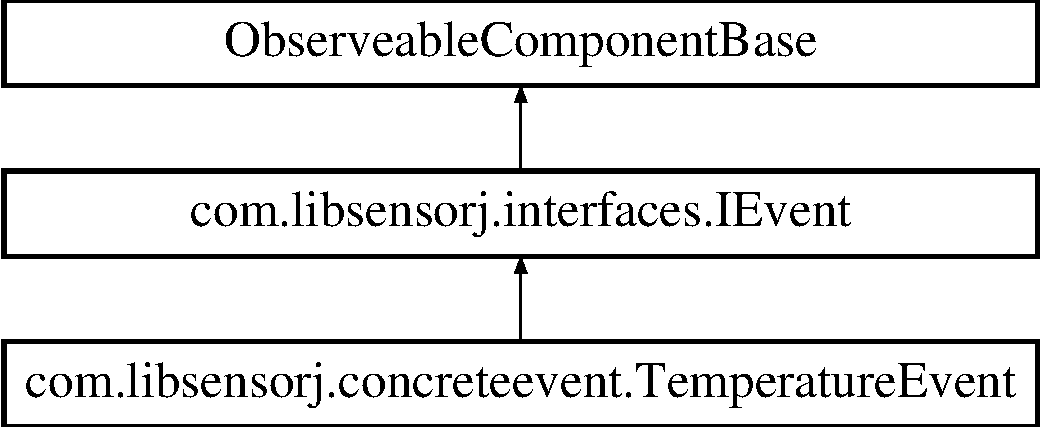
\includegraphics[height=3.000000cm]{classcom_1_1libsensorj_1_1concreteevent_1_1TemperatureEvent}
\end{center}
\end{figure}
\subsection*{Public Member Functions}
\begin{DoxyCompactItemize}
\item 
void \hyperlink{classcom_1_1libsensorj_1_1concreteevent_1_1TemperatureEvent_ad3499315aef403dfde60cf7d9a42c8cf}{attach} (\hyperlink{classcom_1_1libsensorj_1_1model_1_1Observer}{Observer} obsever)
\item 
void \hyperlink{classcom_1_1libsensorj_1_1concreteevent_1_1TemperatureEvent_a7332f144af23c349f39dd714de9c07b9}{detach} (\hyperlink{classcom_1_1libsensorj_1_1model_1_1Observer}{Observer} obsever)
\item 
void \hyperlink{classcom_1_1libsensorj_1_1concreteevent_1_1TemperatureEvent_ac0fe5a9964739808ece4fc9f2562dca5}{trigger} ()
\end{DoxyCompactItemize}


\subsection{Detailed Description}
The Class \hyperlink{classcom_1_1libsensorj_1_1concreteevent_1_1TemperatureEvent}{Temperature\+Event}. 

\subsection{Member Function Documentation}
\hypertarget{classcom_1_1libsensorj_1_1concreteevent_1_1TemperatureEvent_ad3499315aef403dfde60cf7d9a42c8cf}{}\index{com\+::libsensorj\+::concreteevent\+::\+Temperature\+Event@{com\+::libsensorj\+::concreteevent\+::\+Temperature\+Event}!attach@{attach}}
\index{attach@{attach}!com\+::libsensorj\+::concreteevent\+::\+Temperature\+Event@{com\+::libsensorj\+::concreteevent\+::\+Temperature\+Event}}
\subsubsection[{attach}]{\setlength{\rightskip}{0pt plus 5cm}void com.\+libsensorj.\+concreteevent.\+Temperature\+Event.\+attach (
\begin{DoxyParamCaption}
\item[{{\bf Observer}}]{obsever}
\end{DoxyParamCaption}
)}\label{classcom_1_1libsensorj_1_1concreteevent_1_1TemperatureEvent_ad3499315aef403dfde60cf7d9a42c8cf}
\hypertarget{classcom_1_1libsensorj_1_1concreteevent_1_1TemperatureEvent_a7332f144af23c349f39dd714de9c07b9}{}\index{com\+::libsensorj\+::concreteevent\+::\+Temperature\+Event@{com\+::libsensorj\+::concreteevent\+::\+Temperature\+Event}!detach@{detach}}
\index{detach@{detach}!com\+::libsensorj\+::concreteevent\+::\+Temperature\+Event@{com\+::libsensorj\+::concreteevent\+::\+Temperature\+Event}}
\subsubsection[{detach}]{\setlength{\rightskip}{0pt plus 5cm}void com.\+libsensorj.\+concreteevent.\+Temperature\+Event.\+detach (
\begin{DoxyParamCaption}
\item[{{\bf Observer}}]{obsever}
\end{DoxyParamCaption}
)}\label{classcom_1_1libsensorj_1_1concreteevent_1_1TemperatureEvent_a7332f144af23c349f39dd714de9c07b9}
\hypertarget{classcom_1_1libsensorj_1_1concreteevent_1_1TemperatureEvent_ac0fe5a9964739808ece4fc9f2562dca5}{}\index{com\+::libsensorj\+::concreteevent\+::\+Temperature\+Event@{com\+::libsensorj\+::concreteevent\+::\+Temperature\+Event}!trigger@{trigger}}
\index{trigger@{trigger}!com\+::libsensorj\+::concreteevent\+::\+Temperature\+Event@{com\+::libsensorj\+::concreteevent\+::\+Temperature\+Event}}
\subsubsection[{trigger}]{\setlength{\rightskip}{0pt plus 5cm}void com.\+libsensorj.\+concreteevent.\+Temperature\+Event.\+trigger (
\begin{DoxyParamCaption}
{}
\end{DoxyParamCaption}
)}\label{classcom_1_1libsensorj_1_1concreteevent_1_1TemperatureEvent_ac0fe5a9964739808ece4fc9f2562dca5}


The documentation for this class was generated from the following file\+:\begin{DoxyCompactItemize}
\item 
main/java/com/libsensorj/concreteevent/\hyperlink{TemperatureEvent_8java}{Temperature\+Event.\+java}\end{DoxyCompactItemize}

\hypertarget{classcom_1_1libsensorj_1_1concretefactory_1_1TemperatureSensorFactory}{}\section{com.\+libsensorj.\+concretefactory.\+Temperature\+Sensor\+Factory Class Reference}
\label{classcom_1_1libsensorj_1_1concretefactory_1_1TemperatureSensorFactory}\index{com.\+libsensorj.\+concretefactory.\+Temperature\+Sensor\+Factory@{com.\+libsensorj.\+concretefactory.\+Temperature\+Sensor\+Factory}}
Inheritance diagram for com.\+libsensorj.\+concretefactory.\+Temperature\+Sensor\+Factory\+:\begin{figure}[H]
\begin{center}
\leavevmode
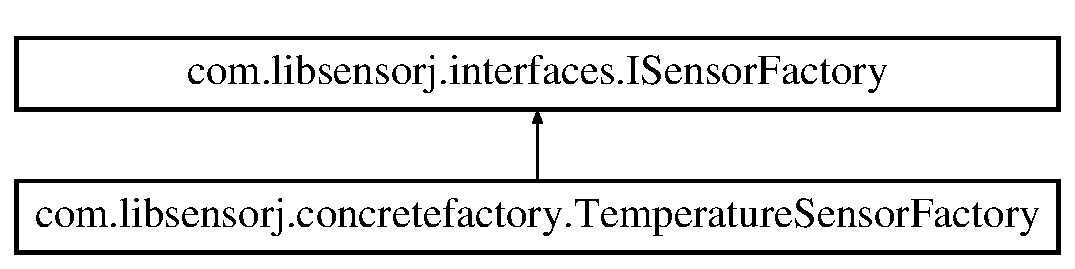
\includegraphics[height=2.000000cm]{classcom_1_1libsensorj_1_1concretefactory_1_1TemperatureSensorFactory}
\end{center}
\end{figure}
\subsection*{Public Member Functions}
\begin{DoxyCompactItemize}
\item 
\hyperlink{interfacecom_1_1libsensorj_1_1interfaces_1_1ISensor}{I\+Sensor} \hyperlink{classcom_1_1libsensorj_1_1concretefactory_1_1TemperatureSensorFactory_aeba8598ebe5c182154f63e0c94abdd70}{create\+Sensor} ()
\item 
\hyperlink{interfacecom_1_1libsensorj_1_1interfaces_1_1IEvent}{I\+Event} \hyperlink{classcom_1_1libsensorj_1_1concretefactory_1_1TemperatureSensorFactory_adb3d5716b5e55f4fc037c0a95ec99688}{create\+Event} ()
\end{DoxyCompactItemize}


\subsection{Member Function Documentation}
\hypertarget{classcom_1_1libsensorj_1_1concretefactory_1_1TemperatureSensorFactory_adb3d5716b5e55f4fc037c0a95ec99688}{}\index{com\+::libsensorj\+::concretefactory\+::\+Temperature\+Sensor\+Factory@{com\+::libsensorj\+::concretefactory\+::\+Temperature\+Sensor\+Factory}!create\+Event@{create\+Event}}
\index{create\+Event@{create\+Event}!com\+::libsensorj\+::concretefactory\+::\+Temperature\+Sensor\+Factory@{com\+::libsensorj\+::concretefactory\+::\+Temperature\+Sensor\+Factory}}
\subsubsection[{create\+Event}]{\setlength{\rightskip}{0pt plus 5cm}{\bf I\+Event} com.\+libsensorj.\+concretefactory.\+Temperature\+Sensor\+Factory.\+create\+Event (
\begin{DoxyParamCaption}
{}
\end{DoxyParamCaption}
)}\label{classcom_1_1libsensorj_1_1concretefactory_1_1TemperatureSensorFactory_adb3d5716b5e55f4fc037c0a95ec99688}


Implements \hyperlink{interfacecom_1_1libsensorj_1_1interfaces_1_1ISensorFactory_a2b074d01287a4e64677097255ba9e768}{com.\+libsensorj.\+interfaces.\+I\+Sensor\+Factory}.

\hypertarget{classcom_1_1libsensorj_1_1concretefactory_1_1TemperatureSensorFactory_aeba8598ebe5c182154f63e0c94abdd70}{}\index{com\+::libsensorj\+::concretefactory\+::\+Temperature\+Sensor\+Factory@{com\+::libsensorj\+::concretefactory\+::\+Temperature\+Sensor\+Factory}!create\+Sensor@{create\+Sensor}}
\index{create\+Sensor@{create\+Sensor}!com\+::libsensorj\+::concretefactory\+::\+Temperature\+Sensor\+Factory@{com\+::libsensorj\+::concretefactory\+::\+Temperature\+Sensor\+Factory}}
\subsubsection[{create\+Sensor}]{\setlength{\rightskip}{0pt plus 5cm}{\bf I\+Sensor} com.\+libsensorj.\+concretefactory.\+Temperature\+Sensor\+Factory.\+create\+Sensor (
\begin{DoxyParamCaption}
{}
\end{DoxyParamCaption}
)}\label{classcom_1_1libsensorj_1_1concretefactory_1_1TemperatureSensorFactory_aeba8598ebe5c182154f63e0c94abdd70}


Implements \hyperlink{interfacecom_1_1libsensorj_1_1interfaces_1_1ISensorFactory_ac14c6d566c37c6a79c6db1e85634f25d}{com.\+libsensorj.\+interfaces.\+I\+Sensor\+Factory}.



The documentation for this class was generated from the following file\+:\begin{DoxyCompactItemize}
\item 
main/java/com/libsensorj/concretefactory/\hyperlink{TemperatureSensorFactory_8java}{Temperature\+Sensor\+Factory.\+java}\end{DoxyCompactItemize}

\hypertarget{classcom_1_1libsensorj_1_1concretesensor_1_1UltrasonicHcsr04}{}\section{com.\+libsensorj.\+concretesensor.\+Ultrasonic\+Hcsr04 Class Reference}
\label{classcom_1_1libsensorj_1_1concretesensor_1_1UltrasonicHcsr04}\index{com.\+libsensorj.\+concretesensor.\+Ultrasonic\+Hcsr04@{com.\+libsensorj.\+concretesensor.\+Ultrasonic\+Hcsr04}}
Inheritance diagram for com.\+libsensorj.\+concretesensor.\+Ultrasonic\+Hcsr04\+:\begin{figure}[H]
\begin{center}
\leavevmode
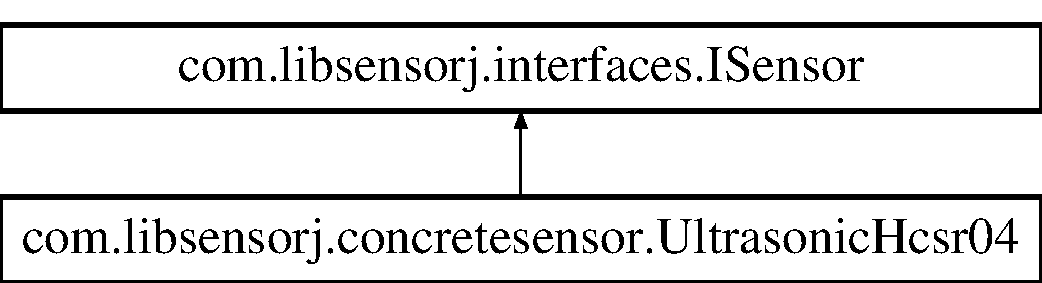
\includegraphics[height=2.000000cm]{classcom_1_1libsensorj_1_1concretesensor_1_1UltrasonicHcsr04}
\end{center}
\end{figure}
\subsection*{Public Member Functions}
\begin{DoxyCompactItemize}
\item 
\hyperlink{classcom_1_1libsensorj_1_1concretesensor_1_1UltrasonicHcsr04_a7e02068d9acb1b3cf1d15d45afbf377b}{Ultrasonic\+Hcsr04} ()
\item 
\hyperlink{classcom_1_1libsensorj_1_1concretesensor_1_1UltrasonicHcsr04_a14e708bf4eb89a2ceb0037fcb837522c}{Ultrasonic\+Hcsr04} (int \hyperlink{classcom_1_1libsensorj_1_1concretesensor_1_1UltrasonicHcsr04_a13705a8251de22d0f52caa3e17d23376}{trigger}, int \hyperlink{classcom_1_1libsensorj_1_1concretesensor_1_1UltrasonicHcsr04_a3695a560e3157a5e6f7896532d717456}{echo})
\item 
\hyperlink{classcom_1_1libsensorj_1_1concretesensor_1_1UltrasonicHcsr04_ae00a91eaf7e5c08695c50a670698ed5f}{Ultrasonic\+Hcsr04} (Pin \hyperlink{classcom_1_1libsensorj_1_1concretesensor_1_1UltrasonicHcsr04_a13705a8251de22d0f52caa3e17d23376}{trigger}, Pin \hyperlink{classcom_1_1libsensorj_1_1concretesensor_1_1UltrasonicHcsr04_a3695a560e3157a5e6f7896532d717456}{echo})
\item 
void \hyperlink{classcom_1_1libsensorj_1_1concretesensor_1_1UltrasonicHcsr04_a170167614b330d79518647a9a9722b62}{get\+Instance} ()
\item 
double \hyperlink{classcom_1_1libsensorj_1_1concretesensor_1_1UltrasonicHcsr04_aec68f4aadd8faa618025dfa37c89c696}{get\+Range} ()
\end{DoxyCompactItemize}
\subsection*{Private Attributes}
\begin{DoxyCompactItemize}
\item 
double \hyperlink{classcom_1_1libsensorj_1_1concretesensor_1_1UltrasonicHcsr04_aad32f417f9106fa8f3f2e2a7416f033b}{result} = 0
\item 
Gpio\+Pin\+Digital\+Output \hyperlink{classcom_1_1libsensorj_1_1concretesensor_1_1UltrasonicHcsr04_a13705a8251de22d0f52caa3e17d23376}{trigger}
\item 
Gpio\+Pin\+Digital\+Input \hyperlink{classcom_1_1libsensorj_1_1concretesensor_1_1UltrasonicHcsr04_a3695a560e3157a5e6f7896532d717456}{echo}
\end{DoxyCompactItemize}
\subsection*{Static Private Attributes}
\begin{DoxyCompactItemize}
\item 
static final int \hyperlink{classcom_1_1libsensorj_1_1concretesensor_1_1UltrasonicHcsr04_aa04a319fc4ef2ccf8de8a70bf27da2da}{T\+W\+E\+N\+T\+Y} = 20
\item 
static final int \hyperlink{classcom_1_1libsensorj_1_1concretesensor_1_1UltrasonicHcsr04_a7106eaa9f89d876a4749d502232964df}{F\+O\+R\+T\+Y} = 40
\item 
static final int \hyperlink{classcom_1_1libsensorj_1_1concretesensor_1_1UltrasonicHcsr04_a25452283296d3780a7fefbfa20e40a93}{T\+H\+I\+R\+T\+Y\+\_\+\+E\+I\+G\+H\+T} = 38
\item 
static final double \hyperlink{classcom_1_1libsensorj_1_1concretesensor_1_1UltrasonicHcsr04_a0483c4e470b1ab9e1a437fbeec6595e9}{D\+I\+S\+T\+A\+N\+C\+E\+\_\+\+F\+A\+C\+T\+O\+R} = 165.\+7
\item 
static final Logger \hyperlink{classcom_1_1libsensorj_1_1concretesensor_1_1UltrasonicHcsr04_a9a3534d952f2668b69b0888b9e929abb}{L\+O\+G\+G\+E\+R}
\end{DoxyCompactItemize}


\subsection{Detailed Description}
The Class \hyperlink{classcom_1_1libsensorj_1_1concretesensor_1_1UltrasonicHcsr04}{Ultrasonic\+Hcsr04}. 

\subsection{Constructor \& Destructor Documentation}
\hypertarget{classcom_1_1libsensorj_1_1concretesensor_1_1UltrasonicHcsr04_a7e02068d9acb1b3cf1d15d45afbf377b}{}\index{com\+::libsensorj\+::concretesensor\+::\+Ultrasonic\+Hcsr04@{com\+::libsensorj\+::concretesensor\+::\+Ultrasonic\+Hcsr04}!Ultrasonic\+Hcsr04@{Ultrasonic\+Hcsr04}}
\index{Ultrasonic\+Hcsr04@{Ultrasonic\+Hcsr04}!com\+::libsensorj\+::concretesensor\+::\+Ultrasonic\+Hcsr04@{com\+::libsensorj\+::concretesensor\+::\+Ultrasonic\+Hcsr04}}
\subsubsection[{Ultrasonic\+Hcsr04}]{\setlength{\rightskip}{0pt plus 5cm}com.\+libsensorj.\+concretesensor.\+Ultrasonic\+Hcsr04.\+Ultrasonic\+Hcsr04 (
\begin{DoxyParamCaption}
{}
\end{DoxyParamCaption}
)}\label{classcom_1_1libsensorj_1_1concretesensor_1_1UltrasonicHcsr04_a7e02068d9acb1b3cf1d15d45afbf377b}
Instantiates a new ultrasonic hcsr04. \hypertarget{classcom_1_1libsensorj_1_1concretesensor_1_1UltrasonicHcsr04_a14e708bf4eb89a2ceb0037fcb837522c}{}\index{com\+::libsensorj\+::concretesensor\+::\+Ultrasonic\+Hcsr04@{com\+::libsensorj\+::concretesensor\+::\+Ultrasonic\+Hcsr04}!Ultrasonic\+Hcsr04@{Ultrasonic\+Hcsr04}}
\index{Ultrasonic\+Hcsr04@{Ultrasonic\+Hcsr04}!com\+::libsensorj\+::concretesensor\+::\+Ultrasonic\+Hcsr04@{com\+::libsensorj\+::concretesensor\+::\+Ultrasonic\+Hcsr04}}
\subsubsection[{Ultrasonic\+Hcsr04}]{\setlength{\rightskip}{0pt plus 5cm}com.\+libsensorj.\+concretesensor.\+Ultrasonic\+Hcsr04.\+Ultrasonic\+Hcsr04 (
\begin{DoxyParamCaption}
\item[{int}]{trigger, }
\item[{int}]{echo}
\end{DoxyParamCaption}
)}\label{classcom_1_1libsensorj_1_1concretesensor_1_1UltrasonicHcsr04_a14e708bf4eb89a2ceb0037fcb837522c}
Instantiates a new ultrasonic hcsr04.


\begin{DoxyParams}{Parameters}
{\em trigger} & the trigger pin \\
\hline
{\em echo} & the echo pin \\
\hline
\end{DoxyParams}
\hypertarget{classcom_1_1libsensorj_1_1concretesensor_1_1UltrasonicHcsr04_ae00a91eaf7e5c08695c50a670698ed5f}{}\index{com\+::libsensorj\+::concretesensor\+::\+Ultrasonic\+Hcsr04@{com\+::libsensorj\+::concretesensor\+::\+Ultrasonic\+Hcsr04}!Ultrasonic\+Hcsr04@{Ultrasonic\+Hcsr04}}
\index{Ultrasonic\+Hcsr04@{Ultrasonic\+Hcsr04}!com\+::libsensorj\+::concretesensor\+::\+Ultrasonic\+Hcsr04@{com\+::libsensorj\+::concretesensor\+::\+Ultrasonic\+Hcsr04}}
\subsubsection[{Ultrasonic\+Hcsr04}]{\setlength{\rightskip}{0pt plus 5cm}com.\+libsensorj.\+concretesensor.\+Ultrasonic\+Hcsr04.\+Ultrasonic\+Hcsr04 (
\begin{DoxyParamCaption}
\item[{Pin}]{trigger, }
\item[{Pin}]{echo}
\end{DoxyParamCaption}
)}\label{classcom_1_1libsensorj_1_1concretesensor_1_1UltrasonicHcsr04_ae00a91eaf7e5c08695c50a670698ed5f}
Instantiates a new ultrasonic hcsr04.


\begin{DoxyParams}{Parameters}
{\em \+\_\+trigger} & the trigger pin \\
\hline
{\em \+\_\+echo} & the echo pin \\
\hline
\end{DoxyParams}


\subsection{Member Function Documentation}
\hypertarget{classcom_1_1libsensorj_1_1concretesensor_1_1UltrasonicHcsr04_a170167614b330d79518647a9a9722b62}{}\index{com\+::libsensorj\+::concretesensor\+::\+Ultrasonic\+Hcsr04@{com\+::libsensorj\+::concretesensor\+::\+Ultrasonic\+Hcsr04}!get\+Instance@{get\+Instance}}
\index{get\+Instance@{get\+Instance}!com\+::libsensorj\+::concretesensor\+::\+Ultrasonic\+Hcsr04@{com\+::libsensorj\+::concretesensor\+::\+Ultrasonic\+Hcsr04}}
\subsubsection[{get\+Instance}]{\setlength{\rightskip}{0pt plus 5cm}void com.\+libsensorj.\+concretesensor.\+Ultrasonic\+Hcsr04.\+get\+Instance (
\begin{DoxyParamCaption}
{}
\end{DoxyParamCaption}
)}\label{classcom_1_1libsensorj_1_1concretesensor_1_1UltrasonicHcsr04_a170167614b330d79518647a9a9722b62}
Gets the single instance of I\+Sensor.

\begin{DoxyReturn}{Returns}
single instance of I\+Sensor 
\end{DoxyReturn}


Implements \hyperlink{interfacecom_1_1libsensorj_1_1interfaces_1_1ISensor_a3c3db93a33adecde81a528651790f75e}{com.\+libsensorj.\+interfaces.\+I\+Sensor}.

\hypertarget{classcom_1_1libsensorj_1_1concretesensor_1_1UltrasonicHcsr04_aec68f4aadd8faa618025dfa37c89c696}{}\index{com\+::libsensorj\+::concretesensor\+::\+Ultrasonic\+Hcsr04@{com\+::libsensorj\+::concretesensor\+::\+Ultrasonic\+Hcsr04}!get\+Range@{get\+Range}}
\index{get\+Range@{get\+Range}!com\+::libsensorj\+::concretesensor\+::\+Ultrasonic\+Hcsr04@{com\+::libsensorj\+::concretesensor\+::\+Ultrasonic\+Hcsr04}}
\subsubsection[{get\+Range}]{\setlength{\rightskip}{0pt plus 5cm}double com.\+libsensorj.\+concretesensor.\+Ultrasonic\+Hcsr04.\+get\+Range (
\begin{DoxyParamCaption}
{}
\end{DoxyParamCaption}
)}\label{classcom_1_1libsensorj_1_1concretesensor_1_1UltrasonicHcsr04_aec68f4aadd8faa618025dfa37c89c696}
Gets the range.

\begin{DoxyReturn}{Returns}
the range 
\end{DoxyReturn}


\subsection{Member Data Documentation}
\hypertarget{classcom_1_1libsensorj_1_1concretesensor_1_1UltrasonicHcsr04_a0483c4e470b1ab9e1a437fbeec6595e9}{}\index{com\+::libsensorj\+::concretesensor\+::\+Ultrasonic\+Hcsr04@{com\+::libsensorj\+::concretesensor\+::\+Ultrasonic\+Hcsr04}!D\+I\+S\+T\+A\+N\+C\+E\+\_\+\+F\+A\+C\+T\+O\+R@{D\+I\+S\+T\+A\+N\+C\+E\+\_\+\+F\+A\+C\+T\+O\+R}}
\index{D\+I\+S\+T\+A\+N\+C\+E\+\_\+\+F\+A\+C\+T\+O\+R@{D\+I\+S\+T\+A\+N\+C\+E\+\_\+\+F\+A\+C\+T\+O\+R}!com\+::libsensorj\+::concretesensor\+::\+Ultrasonic\+Hcsr04@{com\+::libsensorj\+::concretesensor\+::\+Ultrasonic\+Hcsr04}}
\subsubsection[{D\+I\+S\+T\+A\+N\+C\+E\+\_\+\+F\+A\+C\+T\+O\+R}]{\setlength{\rightskip}{0pt plus 5cm}final double com.\+libsensorj.\+concretesensor.\+Ultrasonic\+Hcsr04.\+D\+I\+S\+T\+A\+N\+C\+E\+\_\+\+F\+A\+C\+T\+O\+R = 165.\+7\hspace{0.3cm}{\ttfamily [static]}, {\ttfamily [private]}}\label{classcom_1_1libsensorj_1_1concretesensor_1_1UltrasonicHcsr04_a0483c4e470b1ab9e1a437fbeec6595e9}
The Constant D\+I\+S\+T\+A\+N\+C\+E\+\_\+\+F\+A\+C\+T\+O\+R. \hypertarget{classcom_1_1libsensorj_1_1concretesensor_1_1UltrasonicHcsr04_a3695a560e3157a5e6f7896532d717456}{}\index{com\+::libsensorj\+::concretesensor\+::\+Ultrasonic\+Hcsr04@{com\+::libsensorj\+::concretesensor\+::\+Ultrasonic\+Hcsr04}!echo@{echo}}
\index{echo@{echo}!com\+::libsensorj\+::concretesensor\+::\+Ultrasonic\+Hcsr04@{com\+::libsensorj\+::concretesensor\+::\+Ultrasonic\+Hcsr04}}
\subsubsection[{echo}]{\setlength{\rightskip}{0pt plus 5cm}Gpio\+Pin\+Digital\+Input com.\+libsensorj.\+concretesensor.\+Ultrasonic\+Hcsr04.\+echo\hspace{0.3cm}{\ttfamily [private]}}\label{classcom_1_1libsensorj_1_1concretesensor_1_1UltrasonicHcsr04_a3695a560e3157a5e6f7896532d717456}
The echo. \hypertarget{classcom_1_1libsensorj_1_1concretesensor_1_1UltrasonicHcsr04_a7106eaa9f89d876a4749d502232964df}{}\index{com\+::libsensorj\+::concretesensor\+::\+Ultrasonic\+Hcsr04@{com\+::libsensorj\+::concretesensor\+::\+Ultrasonic\+Hcsr04}!F\+O\+R\+T\+Y@{F\+O\+R\+T\+Y}}
\index{F\+O\+R\+T\+Y@{F\+O\+R\+T\+Y}!com\+::libsensorj\+::concretesensor\+::\+Ultrasonic\+Hcsr04@{com\+::libsensorj\+::concretesensor\+::\+Ultrasonic\+Hcsr04}}
\subsubsection[{F\+O\+R\+T\+Y}]{\setlength{\rightskip}{0pt plus 5cm}final int com.\+libsensorj.\+concretesensor.\+Ultrasonic\+Hcsr04.\+F\+O\+R\+T\+Y = 40\hspace{0.3cm}{\ttfamily [static]}, {\ttfamily [private]}}\label{classcom_1_1libsensorj_1_1concretesensor_1_1UltrasonicHcsr04_a7106eaa9f89d876a4749d502232964df}
The Constant F\+O\+R\+T\+Y. \hypertarget{classcom_1_1libsensorj_1_1concretesensor_1_1UltrasonicHcsr04_a9a3534d952f2668b69b0888b9e929abb}{}\index{com\+::libsensorj\+::concretesensor\+::\+Ultrasonic\+Hcsr04@{com\+::libsensorj\+::concretesensor\+::\+Ultrasonic\+Hcsr04}!L\+O\+G\+G\+E\+R@{L\+O\+G\+G\+E\+R}}
\index{L\+O\+G\+G\+E\+R@{L\+O\+G\+G\+E\+R}!com\+::libsensorj\+::concretesensor\+::\+Ultrasonic\+Hcsr04@{com\+::libsensorj\+::concretesensor\+::\+Ultrasonic\+Hcsr04}}
\subsubsection[{L\+O\+G\+G\+E\+R}]{\setlength{\rightskip}{0pt plus 5cm}final Logger com.\+libsensorj.\+concretesensor.\+Ultrasonic\+Hcsr04.\+L\+O\+G\+G\+E\+R\hspace{0.3cm}{\ttfamily [static]}, {\ttfamily [private]}}\label{classcom_1_1libsensorj_1_1concretesensor_1_1UltrasonicHcsr04_a9a3534d952f2668b69b0888b9e929abb}
{\bfseries Initial value\+:}
\begin{DoxyCode}
= LogManager
            .getLogger(\hyperlink{classcom_1_1libsensorj_1_1concretesensor_1_1UltrasonicHcsr04_a7e02068d9acb1b3cf1d15d45afbf377b}{UltrasonicHcsr04}.class.getName())
\end{DoxyCode}
The Constant L\+O\+G\+G\+E\+R. \hypertarget{classcom_1_1libsensorj_1_1concretesensor_1_1UltrasonicHcsr04_aad32f417f9106fa8f3f2e2a7416f033b}{}\index{com\+::libsensorj\+::concretesensor\+::\+Ultrasonic\+Hcsr04@{com\+::libsensorj\+::concretesensor\+::\+Ultrasonic\+Hcsr04}!result@{result}}
\index{result@{result}!com\+::libsensorj\+::concretesensor\+::\+Ultrasonic\+Hcsr04@{com\+::libsensorj\+::concretesensor\+::\+Ultrasonic\+Hcsr04}}
\subsubsection[{result}]{\setlength{\rightskip}{0pt plus 5cm}double com.\+libsensorj.\+concretesensor.\+Ultrasonic\+Hcsr04.\+result = 0\hspace{0.3cm}{\ttfamily [private]}}\label{classcom_1_1libsensorj_1_1concretesensor_1_1UltrasonicHcsr04_aad32f417f9106fa8f3f2e2a7416f033b}
The result. \hypertarget{classcom_1_1libsensorj_1_1concretesensor_1_1UltrasonicHcsr04_a25452283296d3780a7fefbfa20e40a93}{}\index{com\+::libsensorj\+::concretesensor\+::\+Ultrasonic\+Hcsr04@{com\+::libsensorj\+::concretesensor\+::\+Ultrasonic\+Hcsr04}!T\+H\+I\+R\+T\+Y\+\_\+\+E\+I\+G\+H\+T@{T\+H\+I\+R\+T\+Y\+\_\+\+E\+I\+G\+H\+T}}
\index{T\+H\+I\+R\+T\+Y\+\_\+\+E\+I\+G\+H\+T@{T\+H\+I\+R\+T\+Y\+\_\+\+E\+I\+G\+H\+T}!com\+::libsensorj\+::concretesensor\+::\+Ultrasonic\+Hcsr04@{com\+::libsensorj\+::concretesensor\+::\+Ultrasonic\+Hcsr04}}
\subsubsection[{T\+H\+I\+R\+T\+Y\+\_\+\+E\+I\+G\+H\+T}]{\setlength{\rightskip}{0pt plus 5cm}final int com.\+libsensorj.\+concretesensor.\+Ultrasonic\+Hcsr04.\+T\+H\+I\+R\+T\+Y\+\_\+\+E\+I\+G\+H\+T = 38\hspace{0.3cm}{\ttfamily [static]}, {\ttfamily [private]}}\label{classcom_1_1libsensorj_1_1concretesensor_1_1UltrasonicHcsr04_a25452283296d3780a7fefbfa20e40a93}
The Constant T\+H\+I\+R\+T\+Y\+\_\+\+E\+I\+G\+H\+T. \hypertarget{classcom_1_1libsensorj_1_1concretesensor_1_1UltrasonicHcsr04_a13705a8251de22d0f52caa3e17d23376}{}\index{com\+::libsensorj\+::concretesensor\+::\+Ultrasonic\+Hcsr04@{com\+::libsensorj\+::concretesensor\+::\+Ultrasonic\+Hcsr04}!trigger@{trigger}}
\index{trigger@{trigger}!com\+::libsensorj\+::concretesensor\+::\+Ultrasonic\+Hcsr04@{com\+::libsensorj\+::concretesensor\+::\+Ultrasonic\+Hcsr04}}
\subsubsection[{trigger}]{\setlength{\rightskip}{0pt plus 5cm}Gpio\+Pin\+Digital\+Output com.\+libsensorj.\+concretesensor.\+Ultrasonic\+Hcsr04.\+trigger\hspace{0.3cm}{\ttfamily [private]}}\label{classcom_1_1libsensorj_1_1concretesensor_1_1UltrasonicHcsr04_a13705a8251de22d0f52caa3e17d23376}
The trigger. \hypertarget{classcom_1_1libsensorj_1_1concretesensor_1_1UltrasonicHcsr04_aa04a319fc4ef2ccf8de8a70bf27da2da}{}\index{com\+::libsensorj\+::concretesensor\+::\+Ultrasonic\+Hcsr04@{com\+::libsensorj\+::concretesensor\+::\+Ultrasonic\+Hcsr04}!T\+W\+E\+N\+T\+Y@{T\+W\+E\+N\+T\+Y}}
\index{T\+W\+E\+N\+T\+Y@{T\+W\+E\+N\+T\+Y}!com\+::libsensorj\+::concretesensor\+::\+Ultrasonic\+Hcsr04@{com\+::libsensorj\+::concretesensor\+::\+Ultrasonic\+Hcsr04}}
\subsubsection[{T\+W\+E\+N\+T\+Y}]{\setlength{\rightskip}{0pt plus 5cm}final int com.\+libsensorj.\+concretesensor.\+Ultrasonic\+Hcsr04.\+T\+W\+E\+N\+T\+Y = 20\hspace{0.3cm}{\ttfamily [static]}, {\ttfamily [private]}}\label{classcom_1_1libsensorj_1_1concretesensor_1_1UltrasonicHcsr04_aa04a319fc4ef2ccf8de8a70bf27da2da}
The Constant T\+W\+E\+N\+T\+Y. 

The documentation for this class was generated from the following file\+:\begin{DoxyCompactItemize}
\item 
main/java/com/libsensorj/concretesensor/\hyperlink{UltrasonicHcsr04_8java}{Ultrasonic\+Hcsr04.\+java}\end{DoxyCompactItemize}

\hypertarget{classcom_1_1libsensorj_1_1concreteevent_1_1UltrasonicRangeFinderEvent}{}\section{com.\+libsensorj.\+concreteevent.\+Ultrasonic\+Range\+Finder\+Event Class Reference}
\label{classcom_1_1libsensorj_1_1concreteevent_1_1UltrasonicRangeFinderEvent}\index{com.\+libsensorj.\+concreteevent.\+Ultrasonic\+Range\+Finder\+Event@{com.\+libsensorj.\+concreteevent.\+Ultrasonic\+Range\+Finder\+Event}}
Inheritance diagram for com.\+libsensorj.\+concreteevent.\+Ultrasonic\+Range\+Finder\+Event\+:\begin{figure}[H]
\begin{center}
\leavevmode
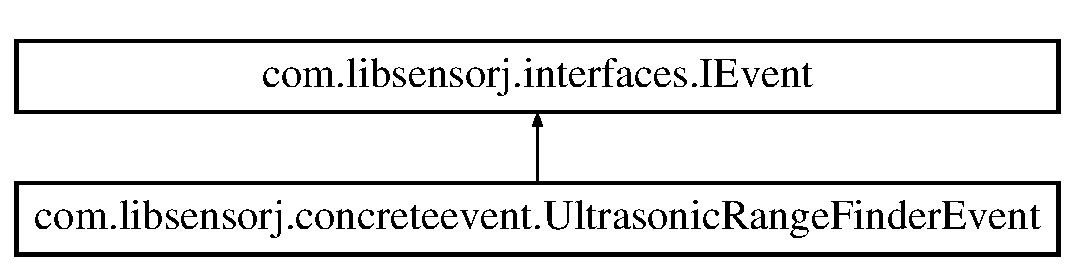
\includegraphics[height=2.000000cm]{classcom_1_1libsensorj_1_1concreteevent_1_1UltrasonicRangeFinderEvent}
\end{center}
\end{figure}
\subsection*{Public Member Functions}
\begin{DoxyCompactItemize}
\item 
void \hyperlink{classcom_1_1libsensorj_1_1concreteevent_1_1UltrasonicRangeFinderEvent_a0b32d3efeb55247269b4f43e4e34fe8e}{attach} (\hyperlink{classcom_1_1libsensorj_1_1model_1_1Observer}{Observer} obsever)
\item 
void \hyperlink{classcom_1_1libsensorj_1_1concreteevent_1_1UltrasonicRangeFinderEvent_ab0647f65e87ff07f61b3e4fe7e1daa19}{detach} (\hyperlink{classcom_1_1libsensorj_1_1model_1_1Observer}{Observer} obsever)
\item 
void \hyperlink{classcom_1_1libsensorj_1_1concreteevent_1_1UltrasonicRangeFinderEvent_a4d1ba316d1d324c4fb6e321e4c7a7b6e}{trigger} ()
\end{DoxyCompactItemize}


\subsection{Member Function Documentation}
\hypertarget{classcom_1_1libsensorj_1_1concreteevent_1_1UltrasonicRangeFinderEvent_a0b32d3efeb55247269b4f43e4e34fe8e}{}\index{com\+::libsensorj\+::concreteevent\+::\+Ultrasonic\+Range\+Finder\+Event@{com\+::libsensorj\+::concreteevent\+::\+Ultrasonic\+Range\+Finder\+Event}!attach@{attach}}
\index{attach@{attach}!com\+::libsensorj\+::concreteevent\+::\+Ultrasonic\+Range\+Finder\+Event@{com\+::libsensorj\+::concreteevent\+::\+Ultrasonic\+Range\+Finder\+Event}}
\subsubsection[{attach}]{\setlength{\rightskip}{0pt plus 5cm}void com.\+libsensorj.\+concreteevent.\+Ultrasonic\+Range\+Finder\+Event.\+attach (
\begin{DoxyParamCaption}
\item[{{\bf Observer}}]{obsever}
\end{DoxyParamCaption}
)}\label{classcom_1_1libsensorj_1_1concreteevent_1_1UltrasonicRangeFinderEvent_a0b32d3efeb55247269b4f43e4e34fe8e}


Implements \hyperlink{interfacecom_1_1libsensorj_1_1interfaces_1_1IEvent_af5af4301ccb6670452419d68baddf372}{com.\+libsensorj.\+interfaces.\+I\+Event}.

\hypertarget{classcom_1_1libsensorj_1_1concreteevent_1_1UltrasonicRangeFinderEvent_ab0647f65e87ff07f61b3e4fe7e1daa19}{}\index{com\+::libsensorj\+::concreteevent\+::\+Ultrasonic\+Range\+Finder\+Event@{com\+::libsensorj\+::concreteevent\+::\+Ultrasonic\+Range\+Finder\+Event}!detach@{detach}}
\index{detach@{detach}!com\+::libsensorj\+::concreteevent\+::\+Ultrasonic\+Range\+Finder\+Event@{com\+::libsensorj\+::concreteevent\+::\+Ultrasonic\+Range\+Finder\+Event}}
\subsubsection[{detach}]{\setlength{\rightskip}{0pt plus 5cm}void com.\+libsensorj.\+concreteevent.\+Ultrasonic\+Range\+Finder\+Event.\+detach (
\begin{DoxyParamCaption}
\item[{{\bf Observer}}]{obsever}
\end{DoxyParamCaption}
)}\label{classcom_1_1libsensorj_1_1concreteevent_1_1UltrasonicRangeFinderEvent_ab0647f65e87ff07f61b3e4fe7e1daa19}


Implements \hyperlink{interfacecom_1_1libsensorj_1_1interfaces_1_1IEvent_a974b07df97fda9f3be8e4afcd46470b2}{com.\+libsensorj.\+interfaces.\+I\+Event}.

\hypertarget{classcom_1_1libsensorj_1_1concreteevent_1_1UltrasonicRangeFinderEvent_a4d1ba316d1d324c4fb6e321e4c7a7b6e}{}\index{com\+::libsensorj\+::concreteevent\+::\+Ultrasonic\+Range\+Finder\+Event@{com\+::libsensorj\+::concreteevent\+::\+Ultrasonic\+Range\+Finder\+Event}!trigger@{trigger}}
\index{trigger@{trigger}!com\+::libsensorj\+::concreteevent\+::\+Ultrasonic\+Range\+Finder\+Event@{com\+::libsensorj\+::concreteevent\+::\+Ultrasonic\+Range\+Finder\+Event}}
\subsubsection[{trigger}]{\setlength{\rightskip}{0pt plus 5cm}void com.\+libsensorj.\+concreteevent.\+Ultrasonic\+Range\+Finder\+Event.\+trigger (
\begin{DoxyParamCaption}
{}
\end{DoxyParamCaption}
)}\label{classcom_1_1libsensorj_1_1concreteevent_1_1UltrasonicRangeFinderEvent_a4d1ba316d1d324c4fb6e321e4c7a7b6e}


Implements \hyperlink{interfacecom_1_1libsensorj_1_1interfaces_1_1IEvent_a861dea0956f77dd82f95e0110b8043b2}{com.\+libsensorj.\+interfaces.\+I\+Event}.



The documentation for this class was generated from the following file\+:\begin{DoxyCompactItemize}
\item 
main/java/com/libsensorj/concreteevent/\hyperlink{UltrasonicRangeFinderEvent_8java}{Ultrasonic\+Range\+Finder\+Event.\+java}\end{DoxyCompactItemize}

\hypertarget{classcom_1_1libsensorj_1_1examples_1_1UltrasonicRangeFinderExample}{}\section{com.\+libsensorj.\+examples.\+Ultrasonic\+Range\+Finder\+Example Class Reference}
\label{classcom_1_1libsensorj_1_1examples_1_1UltrasonicRangeFinderExample}\index{com.\+libsensorj.\+examples.\+Ultrasonic\+Range\+Finder\+Example@{com.\+libsensorj.\+examples.\+Ultrasonic\+Range\+Finder\+Example}}
\subsection*{Static Public Member Functions}
\begin{DoxyCompactItemize}
\item 
static void \hyperlink{classcom_1_1libsensorj_1_1examples_1_1UltrasonicRangeFinderExample_a587a298526337ce9e0d1fbbb9f400180}{main} (String\mbox{[}$\,$\mbox{]} args)
\end{DoxyCompactItemize}
\subsection*{Static Private Attributes}
\begin{DoxyCompactItemize}
\item 
static \hyperlink{interfacecom_1_1libsensorj_1_1interfaces_1_1ISensor}{I\+Sensor} \hyperlink{classcom_1_1libsensorj_1_1examples_1_1UltrasonicRangeFinderExample_af4703590c0c8bce89386204ea46afc76}{hcsr}
\item 
static final Logger \hyperlink{classcom_1_1libsensorj_1_1examples_1_1UltrasonicRangeFinderExample_ac1d433a89455addc211f404fe522f0ec}{L\+O\+G\+G\+E\+R}
\end{DoxyCompactItemize}


\subsection{Detailed Description}
The Class \hyperlink{classcom_1_1libsensorj_1_1examples_1_1UltrasonicRangeFinderExample}{Ultrasonic\+Range\+Finder\+Example}. 

\subsection{Member Function Documentation}
\hypertarget{classcom_1_1libsensorj_1_1examples_1_1UltrasonicRangeFinderExample_a587a298526337ce9e0d1fbbb9f400180}{}\index{com\+::libsensorj\+::examples\+::\+Ultrasonic\+Range\+Finder\+Example@{com\+::libsensorj\+::examples\+::\+Ultrasonic\+Range\+Finder\+Example}!main@{main}}
\index{main@{main}!com\+::libsensorj\+::examples\+::\+Ultrasonic\+Range\+Finder\+Example@{com\+::libsensorj\+::examples\+::\+Ultrasonic\+Range\+Finder\+Example}}
\subsubsection[{main}]{\setlength{\rightskip}{0pt plus 5cm}static void com.\+libsensorj.\+examples.\+Ultrasonic\+Range\+Finder\+Example.\+main (
\begin{DoxyParamCaption}
\item[{String\mbox{[}$\,$\mbox{]}}]{args}
\end{DoxyParamCaption}
)\hspace{0.3cm}{\ttfamily [static]}}\label{classcom_1_1libsensorj_1_1examples_1_1UltrasonicRangeFinderExample_a587a298526337ce9e0d1fbbb9f400180}
The main method.


\begin{DoxyParams}{Parameters}
{\em args} & the arguments \\
\hline
\end{DoxyParams}


\subsection{Member Data Documentation}
\hypertarget{classcom_1_1libsensorj_1_1examples_1_1UltrasonicRangeFinderExample_af4703590c0c8bce89386204ea46afc76}{}\index{com\+::libsensorj\+::examples\+::\+Ultrasonic\+Range\+Finder\+Example@{com\+::libsensorj\+::examples\+::\+Ultrasonic\+Range\+Finder\+Example}!hcsr@{hcsr}}
\index{hcsr@{hcsr}!com\+::libsensorj\+::examples\+::\+Ultrasonic\+Range\+Finder\+Example@{com\+::libsensorj\+::examples\+::\+Ultrasonic\+Range\+Finder\+Example}}
\subsubsection[{hcsr}]{\setlength{\rightskip}{0pt plus 5cm}{\bf I\+Sensor} com.\+libsensorj.\+examples.\+Ultrasonic\+Range\+Finder\+Example.\+hcsr\hspace{0.3cm}{\ttfamily [static]}, {\ttfamily [private]}}\label{classcom_1_1libsensorj_1_1examples_1_1UltrasonicRangeFinderExample_af4703590c0c8bce89386204ea46afc76}
The I\+Sensor hcsr. \hypertarget{classcom_1_1libsensorj_1_1examples_1_1UltrasonicRangeFinderExample_ac1d433a89455addc211f404fe522f0ec}{}\index{com\+::libsensorj\+::examples\+::\+Ultrasonic\+Range\+Finder\+Example@{com\+::libsensorj\+::examples\+::\+Ultrasonic\+Range\+Finder\+Example}!L\+O\+G\+G\+E\+R@{L\+O\+G\+G\+E\+R}}
\index{L\+O\+G\+G\+E\+R@{L\+O\+G\+G\+E\+R}!com\+::libsensorj\+::examples\+::\+Ultrasonic\+Range\+Finder\+Example@{com\+::libsensorj\+::examples\+::\+Ultrasonic\+Range\+Finder\+Example}}
\subsubsection[{L\+O\+G\+G\+E\+R}]{\setlength{\rightskip}{0pt plus 5cm}final Logger com.\+libsensorj.\+examples.\+Ultrasonic\+Range\+Finder\+Example.\+L\+O\+G\+G\+E\+R\hspace{0.3cm}{\ttfamily [static]}, {\ttfamily [private]}}\label{classcom_1_1libsensorj_1_1examples_1_1UltrasonicRangeFinderExample_ac1d433a89455addc211f404fe522f0ec}
{\bfseries Initial value\+:}
\begin{DoxyCode}
= LogManager
            .getLogger(UltrasonicRangeFinderExample.class.getName())
\end{DoxyCode}
The Constant L\+O\+G\+G\+E\+R. 

The documentation for this class was generated from the following file\+:\begin{DoxyCompactItemize}
\item 
main/java/com/libsensorj/examples/\hyperlink{UltrasonicRangeFinderExample_8java}{Ultrasonic\+Range\+Finder\+Example.\+java}\end{DoxyCompactItemize}

\hypertarget{classcom_1_1libsensorj_1_1concretefactory_1_1UltrasonicRangeFinderFactory}{}\section{com.\+libsensorj.\+concretefactory.\+Ultrasonic\+Range\+Finder\+Factory Class Reference}
\label{classcom_1_1libsensorj_1_1concretefactory_1_1UltrasonicRangeFinderFactory}\index{com.\+libsensorj.\+concretefactory.\+Ultrasonic\+Range\+Finder\+Factory@{com.\+libsensorj.\+concretefactory.\+Ultrasonic\+Range\+Finder\+Factory}}
Inheritance diagram for com.\+libsensorj.\+concretefactory.\+Ultrasonic\+Range\+Finder\+Factory\+:\begin{figure}[H]
\begin{center}
\leavevmode
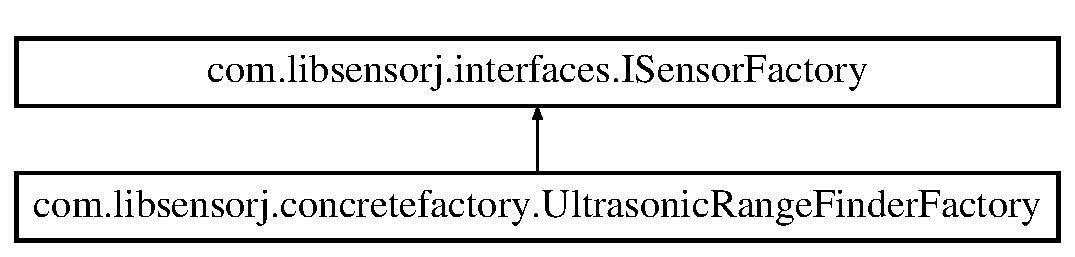
\includegraphics[height=2.000000cm]{classcom_1_1libsensorj_1_1concretefactory_1_1UltrasonicRangeFinderFactory}
\end{center}
\end{figure}
\subsection*{Public Member Functions}
\begin{DoxyCompactItemize}
\item 
\hyperlink{interfacecom_1_1libsensorj_1_1interfaces_1_1ISensor}{I\+Sensor} \hyperlink{classcom_1_1libsensorj_1_1concretefactory_1_1UltrasonicRangeFinderFactory_a3aa6e46ef47bf97355df4d5cfb1b1e01}{create\+Sensor} ()
\item 
\hyperlink{interfacecom_1_1libsensorj_1_1interfaces_1_1IEvent}{I\+Event} \hyperlink{classcom_1_1libsensorj_1_1concretefactory_1_1UltrasonicRangeFinderFactory_a8a7d0c55346f1ab5630a878f6a3175fd}{create\+Event} ()
\end{DoxyCompactItemize}


\subsection{Member Function Documentation}
\hypertarget{classcom_1_1libsensorj_1_1concretefactory_1_1UltrasonicRangeFinderFactory_a8a7d0c55346f1ab5630a878f6a3175fd}{}\index{com\+::libsensorj\+::concretefactory\+::\+Ultrasonic\+Range\+Finder\+Factory@{com\+::libsensorj\+::concretefactory\+::\+Ultrasonic\+Range\+Finder\+Factory}!create\+Event@{create\+Event}}
\index{create\+Event@{create\+Event}!com\+::libsensorj\+::concretefactory\+::\+Ultrasonic\+Range\+Finder\+Factory@{com\+::libsensorj\+::concretefactory\+::\+Ultrasonic\+Range\+Finder\+Factory}}
\subsubsection[{create\+Event}]{\setlength{\rightskip}{0pt plus 5cm}{\bf I\+Event} com.\+libsensorj.\+concretefactory.\+Ultrasonic\+Range\+Finder\+Factory.\+create\+Event (
\begin{DoxyParamCaption}
{}
\end{DoxyParamCaption}
)}\label{classcom_1_1libsensorj_1_1concretefactory_1_1UltrasonicRangeFinderFactory_a8a7d0c55346f1ab5630a878f6a3175fd}


Implements \hyperlink{interfacecom_1_1libsensorj_1_1interfaces_1_1ISensorFactory_a2b074d01287a4e64677097255ba9e768}{com.\+libsensorj.\+interfaces.\+I\+Sensor\+Factory}.

\hypertarget{classcom_1_1libsensorj_1_1concretefactory_1_1UltrasonicRangeFinderFactory_a3aa6e46ef47bf97355df4d5cfb1b1e01}{}\index{com\+::libsensorj\+::concretefactory\+::\+Ultrasonic\+Range\+Finder\+Factory@{com\+::libsensorj\+::concretefactory\+::\+Ultrasonic\+Range\+Finder\+Factory}!create\+Sensor@{create\+Sensor}}
\index{create\+Sensor@{create\+Sensor}!com\+::libsensorj\+::concretefactory\+::\+Ultrasonic\+Range\+Finder\+Factory@{com\+::libsensorj\+::concretefactory\+::\+Ultrasonic\+Range\+Finder\+Factory}}
\subsubsection[{create\+Sensor}]{\setlength{\rightskip}{0pt plus 5cm}{\bf I\+Sensor} com.\+libsensorj.\+concretefactory.\+Ultrasonic\+Range\+Finder\+Factory.\+create\+Sensor (
\begin{DoxyParamCaption}
{}
\end{DoxyParamCaption}
)}\label{classcom_1_1libsensorj_1_1concretefactory_1_1UltrasonicRangeFinderFactory_a3aa6e46ef47bf97355df4d5cfb1b1e01}


Implements \hyperlink{interfacecom_1_1libsensorj_1_1interfaces_1_1ISensorFactory_ac14c6d566c37c6a79c6db1e85634f25d}{com.\+libsensorj.\+interfaces.\+I\+Sensor\+Factory}.



The documentation for this class was generated from the following file\+:\begin{DoxyCompactItemize}
\item 
main/java/com/libsensorj/concretefactory/\hyperlink{UltrasonicRangeFinderFactory_8java}{Ultrasonic\+Range\+Finder\+Factory.\+java}\end{DoxyCompactItemize}

\chapter{File Documentation}
\hypertarget{HumidityEvent_8java}{}\section{main/java/com/libsensorj/concreteevent/\+Humidity\+Event.java File Reference}
\label{HumidityEvent_8java}\index{main/java/com/libsensorj/concreteevent/\+Humidity\+Event.\+java@{main/java/com/libsensorj/concreteevent/\+Humidity\+Event.\+java}}
\subsection*{Classes}
\begin{DoxyCompactItemize}
\item 
class \hyperlink{classcom_1_1libsensorj_1_1concreteevent_1_1HumidityEvent}{com.\+libsensorj.\+concreteevent.\+Humidity\+Event}
\end{DoxyCompactItemize}
\subsection*{Packages}
\begin{DoxyCompactItemize}
\item 
package \hyperlink{namespacecom_1_1libsensorj_1_1concreteevent}{com.\+libsensorj.\+concreteevent}
\end{DoxyCompactItemize}

\hypertarget{TemperatureEvent_8java}{}\section{main/java/com/libsensorj/concreteevent/\+Temperature\+Event.java File Reference}
\label{TemperatureEvent_8java}\index{main/java/com/libsensorj/concreteevent/\+Temperature\+Event.\+java@{main/java/com/libsensorj/concreteevent/\+Temperature\+Event.\+java}}
\subsection*{Classes}
\begin{DoxyCompactItemize}
\item 
class \hyperlink{classcom_1_1libsensorj_1_1concreteevent_1_1TemperatureEvent}{com.\+libsensorj.\+concreteevent.\+Temperature\+Event}
\end{DoxyCompactItemize}
\subsection*{Packages}
\begin{DoxyCompactItemize}
\item 
package \hyperlink{namespacecom_1_1libsensorj_1_1concreteevent}{com.\+libsensorj.\+concreteevent}
\end{DoxyCompactItemize}

\hypertarget{UltrasonicRangeFinderEvent_8java}{}\section{main/java/com/libsensorj/concreteevent/\+Ultrasonic\+Range\+Finder\+Event.java File Reference}
\label{UltrasonicRangeFinderEvent_8java}\index{main/java/com/libsensorj/concreteevent/\+Ultrasonic\+Range\+Finder\+Event.\+java@{main/java/com/libsensorj/concreteevent/\+Ultrasonic\+Range\+Finder\+Event.\+java}}
\subsection*{Classes}
\begin{DoxyCompactItemize}
\item 
class \hyperlink{classcom_1_1libsensorj_1_1concreteevent_1_1UltrasonicRangeFinderEvent}{com.\+libsensorj.\+concreteevent.\+Ultrasonic\+Range\+Finder\+Event}
\end{DoxyCompactItemize}
\subsection*{Packages}
\begin{DoxyCompactItemize}
\item 
package \hyperlink{namespacecom_1_1libsensorj_1_1concreteevent}{com.\+libsensorj.\+concreteevent}
\end{DoxyCompactItemize}

\hypertarget{DHT11V2Factory_8java}{}\section{main/java/com/libsensorj/concretefactory/\+D\+H\+T11\+V2\+Factory.java File Reference}
\label{DHT11V2Factory_8java}\index{main/java/com/libsensorj/concretefactory/\+D\+H\+T11\+V2\+Factory.\+java@{main/java/com/libsensorj/concretefactory/\+D\+H\+T11\+V2\+Factory.\+java}}
\subsection*{Classes}
\begin{DoxyCompactItemize}
\item 
class \hyperlink{classcom_1_1libsensorj_1_1concretefactory_1_1DHT11V2Factory}{com.\+libsensorj.\+concretefactory.\+D\+H\+T11\+V2\+Factory}
\end{DoxyCompactItemize}
\subsection*{Packages}
\begin{DoxyCompactItemize}
\item 
package \hyperlink{namespacecom_1_1libsensorj_1_1concretefactory}{com.\+libsensorj.\+concretefactory}
\end{DoxyCompactItemize}

\hypertarget{DHT11V3Factory_8java}{}\section{main/java/com/libsensorj/concretefactory/\+D\+H\+T11\+V3\+Factory.java File Reference}
\label{DHT11V3Factory_8java}\index{main/java/com/libsensorj/concretefactory/\+D\+H\+T11\+V3\+Factory.\+java@{main/java/com/libsensorj/concretefactory/\+D\+H\+T11\+V3\+Factory.\+java}}
\subsection*{Classes}
\begin{DoxyCompactItemize}
\item 
class \hyperlink{classcom_1_1libsensorj_1_1concretefactory_1_1DHT11V3Factory}{com.\+libsensorj.\+concretefactory.\+D\+H\+T11\+V3\+Factory}
\end{DoxyCompactItemize}
\subsection*{Packages}
\begin{DoxyCompactItemize}
\item 
package \hyperlink{namespacecom_1_1libsensorj_1_1concretefactory}{com.\+libsensorj.\+concretefactory}
\end{DoxyCompactItemize}

\hypertarget{HCSR04DeviceFactory_8java}{}\section{main/java/com/libsensorj/concretefactory/\+H\+C\+S\+R04\+Device\+Factory.java File Reference}
\label{HCSR04DeviceFactory_8java}\index{main/java/com/libsensorj/concretefactory/\+H\+C\+S\+R04\+Device\+Factory.\+java@{main/java/com/libsensorj/concretefactory/\+H\+C\+S\+R04\+Device\+Factory.\+java}}
\subsection*{Classes}
\begin{DoxyCompactItemize}
\item 
class \hyperlink{classcom_1_1libsensorj_1_1concretefactory_1_1HCSR04DeviceFactory}{com.\+libsensorj.\+concretefactory.\+H\+C\+S\+R04\+Device\+Factory}
\end{DoxyCompactItemize}
\subsection*{Packages}
\begin{DoxyCompactItemize}
\item 
package \hyperlink{namespacecom_1_1libsensorj_1_1concretefactory}{com.\+libsensorj.\+concretefactory}
\end{DoxyCompactItemize}

\hypertarget{HumiditySensorFactory_8java}{}\section{main/java/com/libsensorj/concretefactory/\+Humidity\+Sensor\+Factory.java File Reference}
\label{HumiditySensorFactory_8java}\index{main/java/com/libsensorj/concretefactory/\+Humidity\+Sensor\+Factory.\+java@{main/java/com/libsensorj/concretefactory/\+Humidity\+Sensor\+Factory.\+java}}
\subsection*{Classes}
\begin{DoxyCompactItemize}
\item 
class \hyperlink{classcom_1_1libsensorj_1_1concretefactory_1_1HumiditySensorFactory}{com.\+libsensorj.\+concretefactory.\+Humidity\+Sensor\+Factory}
\end{DoxyCompactItemize}
\subsection*{Packages}
\begin{DoxyCompactItemize}
\item 
package \hyperlink{namespacecom_1_1libsensorj_1_1concretefactory}{com.\+libsensorj.\+concretefactory}
\end{DoxyCompactItemize}

\hypertarget{TemperatureSensorFactory_8java}{}\section{main/java/com/libsensorj/concretefactory/\+Temperature\+Sensor\+Factory.java File Reference}
\label{TemperatureSensorFactory_8java}\index{main/java/com/libsensorj/concretefactory/\+Temperature\+Sensor\+Factory.\+java@{main/java/com/libsensorj/concretefactory/\+Temperature\+Sensor\+Factory.\+java}}
\subsection*{Classes}
\begin{DoxyCompactItemize}
\item 
class \hyperlink{classcom_1_1libsensorj_1_1concretefactory_1_1TemperatureSensorFactory}{com.\+libsensorj.\+concretefactory.\+Temperature\+Sensor\+Factory}
\end{DoxyCompactItemize}
\subsection*{Packages}
\begin{DoxyCompactItemize}
\item 
package \hyperlink{namespacecom_1_1libsensorj_1_1concretefactory}{com.\+libsensorj.\+concretefactory}
\end{DoxyCompactItemize}

\hypertarget{UltrasonicRangeFinderFactory_8java}{}\section{main/java/com/libsensorj/concretefactory/\+Ultrasonic\+Range\+Finder\+Factory.java File Reference}
\label{UltrasonicRangeFinderFactory_8java}\index{main/java/com/libsensorj/concretefactory/\+Ultrasonic\+Range\+Finder\+Factory.\+java@{main/java/com/libsensorj/concretefactory/\+Ultrasonic\+Range\+Finder\+Factory.\+java}}
\subsection*{Classes}
\begin{DoxyCompactItemize}
\item 
class \hyperlink{classcom_1_1libsensorj_1_1concretefactory_1_1UltrasonicRangeFinderFactory}{com.\+libsensorj.\+concretefactory.\+Ultrasonic\+Range\+Finder\+Factory}
\end{DoxyCompactItemize}
\subsection*{Packages}
\begin{DoxyCompactItemize}
\item 
package \hyperlink{namespacecom_1_1libsensorj_1_1concretefactory}{com.\+libsensorj.\+concretefactory}
\end{DoxyCompactItemize}

\hypertarget{DHT11_8java}{}\section{main/java/com/libsensorj/concretesensor/\+D\+H\+T11.java File Reference}
\label{DHT11_8java}\index{main/java/com/libsensorj/concretesensor/\+D\+H\+T11.\+java@{main/java/com/libsensorj/concretesensor/\+D\+H\+T11.\+java}}
\subsection*{Classes}
\begin{DoxyCompactItemize}
\item 
class \hyperlink{classcom_1_1libsensorj_1_1concretesensor_1_1DHT11}{com.\+libsensorj.\+concretesensor.\+D\+H\+T11}
\end{DoxyCompactItemize}
\subsection*{Packages}
\begin{DoxyCompactItemize}
\item 
package \hyperlink{namespacecom_1_1libsensorj_1_1concretesensor}{com.\+libsensorj.\+concretesensor}
\end{DoxyCompactItemize}

\hypertarget{DHT11Humidity_8java}{}\section{main/java/com/libsensorj/concretesensor/\+D\+H\+T11\+Humidity.java File Reference}
\label{DHT11Humidity_8java}\index{main/java/com/libsensorj/concretesensor/\+D\+H\+T11\+Humidity.\+java@{main/java/com/libsensorj/concretesensor/\+D\+H\+T11\+Humidity.\+java}}
\subsection*{Classes}
\begin{DoxyCompactItemize}
\item 
class \hyperlink{classcom_1_1libsensorj_1_1concretesensor_1_1DHT11Humidity}{com.\+libsensorj.\+concretesensor.\+D\+H\+T11\+Humidity}
\end{DoxyCompactItemize}
\subsection*{Packages}
\begin{DoxyCompactItemize}
\item 
package \hyperlink{namespacecom_1_1libsensorj_1_1concretesensor}{com.\+libsensorj.\+concretesensor}
\end{DoxyCompactItemize}

\hypertarget{DHT11Temperature_8java}{}\section{main/java/com/libsensorj/concretesensor/\+D\+H\+T11\+Temperature.java File Reference}
\label{DHT11Temperature_8java}\index{main/java/com/libsensorj/concretesensor/\+D\+H\+T11\+Temperature.\+java@{main/java/com/libsensorj/concretesensor/\+D\+H\+T11\+Temperature.\+java}}
\subsection*{Classes}
\begin{DoxyCompactItemize}
\item 
class \hyperlink{classcom_1_1libsensorj_1_1concretesensor_1_1DHT11Temperature}{com.\+libsensorj.\+concretesensor.\+D\+H\+T11\+Temperature}
\end{DoxyCompactItemize}
\subsection*{Packages}
\begin{DoxyCompactItemize}
\item 
package \hyperlink{namespacecom_1_1libsensorj_1_1concretesensor}{com.\+libsensorj.\+concretesensor}
\end{DoxyCompactItemize}

\hypertarget{DHT11V2_8java}{}\section{main/java/com/libsensorj/concretesensor/\+D\+H\+T11\+V2.java File Reference}
\label{DHT11V2_8java}\index{main/java/com/libsensorj/concretesensor/\+D\+H\+T11\+V2.\+java@{main/java/com/libsensorj/concretesensor/\+D\+H\+T11\+V2.\+java}}
\subsection*{Classes}
\begin{DoxyCompactItemize}
\item 
class \hyperlink{classcom_1_1libsensorj_1_1concretesensor_1_1DHT11V2}{com.\+libsensorj.\+concretesensor.\+D\+H\+T11\+V2}
\end{DoxyCompactItemize}
\subsection*{Packages}
\begin{DoxyCompactItemize}
\item 
package \hyperlink{namespacecom_1_1libsensorj_1_1concretesensor}{com.\+libsensorj.\+concretesensor}
\end{DoxyCompactItemize}

\hypertarget{DHT11V3_8java}{}\section{main/java/com/libsensorj/concretesensor/\+D\+H\+T11\+V3.java File Reference}
\label{DHT11V3_8java}\index{main/java/com/libsensorj/concretesensor/\+D\+H\+T11\+V3.\+java@{main/java/com/libsensorj/concretesensor/\+D\+H\+T11\+V3.\+java}}
\subsection*{Classes}
\begin{DoxyCompactItemize}
\item 
class \hyperlink{classcom_1_1libsensorj_1_1concretesensor_1_1DHT11V3}{com.\+libsensorj.\+concretesensor.\+D\+H\+T11\+V3}
\end{DoxyCompactItemize}
\subsection*{Packages}
\begin{DoxyCompactItemize}
\item 
package \hyperlink{namespacecom_1_1libsensorj_1_1concretesensor}{com.\+libsensorj.\+concretesensor}
\end{DoxyCompactItemize}

\hypertarget{HCSR04Device_8java}{}\section{main/java/com/libsensorj/concretesensor/\+H\+C\+S\+R04\+Device.java File Reference}
\label{HCSR04Device_8java}\index{main/java/com/libsensorj/concretesensor/\+H\+C\+S\+R04\+Device.\+java@{main/java/com/libsensorj/concretesensor/\+H\+C\+S\+R04\+Device.\+java}}
\subsection*{Classes}
\begin{DoxyCompactItemize}
\item 
class \hyperlink{classcom_1_1libsensorj_1_1concretesensor_1_1HCSR04Device}{com.\+libsensorj.\+concretesensor.\+H\+C\+S\+R04\+Device}
\end{DoxyCompactItemize}
\subsection*{Packages}
\begin{DoxyCompactItemize}
\item 
package \hyperlink{namespacecom_1_1libsensorj_1_1concretesensor}{com.\+libsensorj.\+concretesensor}
\end{DoxyCompactItemize}

\hypertarget{UltrasonicHcsr04_8java}{}\section{main/java/com/libsensorj/concretesensor/\+Ultrasonic\+Hcsr04.java File Reference}
\label{UltrasonicHcsr04_8java}\index{main/java/com/libsensorj/concretesensor/\+Ultrasonic\+Hcsr04.\+java@{main/java/com/libsensorj/concretesensor/\+Ultrasonic\+Hcsr04.\+java}}
\subsection*{Classes}
\begin{DoxyCompactItemize}
\item 
class \hyperlink{classcom_1_1libsensorj_1_1concretesensor_1_1UltrasonicHcsr04}{com.\+libsensorj.\+concretesensor.\+Ultrasonic\+Hcsr04}
\end{DoxyCompactItemize}
\subsection*{Packages}
\begin{DoxyCompactItemize}
\item 
package \hyperlink{namespacecom_1_1libsensorj_1_1concretesensor}{com.\+libsensorj.\+concretesensor}
\end{DoxyCompactItemize}

\hypertarget{DHT11TemperatureExample_8java}{}\section{main/java/com/libsensorj/examples/\+D\+H\+T11\+Temperature\+Example.java File Reference}
\label{DHT11TemperatureExample_8java}\index{main/java/com/libsensorj/examples/\+D\+H\+T11\+Temperature\+Example.\+java@{main/java/com/libsensorj/examples/\+D\+H\+T11\+Temperature\+Example.\+java}}
\subsection*{Classes}
\begin{DoxyCompactItemize}
\item 
class \hyperlink{classcom_1_1libsensorj_1_1examples_1_1DHT11TemperatureExample}{com.\+libsensorj.\+examples.\+D\+H\+T11\+Temperature\+Example}
\end{DoxyCompactItemize}
\subsection*{Packages}
\begin{DoxyCompactItemize}
\item 
package \hyperlink{namespacecom_1_1libsensorj_1_1examples}{com.\+libsensorj.\+examples}
\end{DoxyCompactItemize}

\hypertarget{DHT11V2Example_8java}{}\section{main/java/com/libsensorj/examples/\+D\+H\+T11\+V2\+Example.java File Reference}
\label{DHT11V2Example_8java}\index{main/java/com/libsensorj/examples/\+D\+H\+T11\+V2\+Example.\+java@{main/java/com/libsensorj/examples/\+D\+H\+T11\+V2\+Example.\+java}}
\subsection*{Classes}
\begin{DoxyCompactItemize}
\item 
class \hyperlink{classcom_1_1libsensorj_1_1examples_1_1DHT11V2Example}{com.\+libsensorj.\+examples.\+D\+H\+T11\+V2\+Example}
\end{DoxyCompactItemize}
\subsection*{Packages}
\begin{DoxyCompactItemize}
\item 
package \hyperlink{namespacecom_1_1libsensorj_1_1examples}{com.\+libsensorj.\+examples}
\end{DoxyCompactItemize}

\hypertarget{DHT11V3Example_8java}{}\section{main/java/com/libsensorj/examples/\+D\+H\+T11\+V3\+Example.java File Reference}
\label{DHT11V3Example_8java}\index{main/java/com/libsensorj/examples/\+D\+H\+T11\+V3\+Example.\+java@{main/java/com/libsensorj/examples/\+D\+H\+T11\+V3\+Example.\+java}}
\subsection*{Classes}
\begin{DoxyCompactItemize}
\item 
class \hyperlink{classcom_1_1libsensorj_1_1examples_1_1DHT11V3Example}{com.\+libsensorj.\+examples.\+D\+H\+T11\+V3\+Example}
\end{DoxyCompactItemize}
\subsection*{Packages}
\begin{DoxyCompactItemize}
\item 
package \hyperlink{namespacecom_1_1libsensorj_1_1examples}{com.\+libsensorj.\+examples}
\end{DoxyCompactItemize}

\hypertarget{HCSR04DeviceExample_8java}{}\section{main/java/com/libsensorj/examples/\+H\+C\+S\+R04\+Device\+Example.java File Reference}
\label{HCSR04DeviceExample_8java}\index{main/java/com/libsensorj/examples/\+H\+C\+S\+R04\+Device\+Example.\+java@{main/java/com/libsensorj/examples/\+H\+C\+S\+R04\+Device\+Example.\+java}}
\subsection*{Classes}
\begin{DoxyCompactItemize}
\item 
class \hyperlink{classcom_1_1libsensorj_1_1examples_1_1HCSR04DeviceExample}{com.\+libsensorj.\+examples.\+H\+C\+S\+R04\+Device\+Example}
\end{DoxyCompactItemize}
\subsection*{Packages}
\begin{DoxyCompactItemize}
\item 
package \hyperlink{namespacecom_1_1libsensorj_1_1examples}{com.\+libsensorj.\+examples}
\end{DoxyCompactItemize}

\hypertarget{UltrasonicRangeFinderExample_8java}{}\section{main/java/com/libsensorj/examples/\+Ultrasonic\+Range\+Finder\+Example.java File Reference}
\label{UltrasonicRangeFinderExample_8java}\index{main/java/com/libsensorj/examples/\+Ultrasonic\+Range\+Finder\+Example.\+java@{main/java/com/libsensorj/examples/\+Ultrasonic\+Range\+Finder\+Example.\+java}}
\subsection*{Classes}
\begin{DoxyCompactItemize}
\item 
class \hyperlink{classcom_1_1libsensorj_1_1examples_1_1UltrasonicRangeFinderExample}{com.\+libsensorj.\+examples.\+Ultrasonic\+Range\+Finder\+Example}
\end{DoxyCompactItemize}
\subsection*{Packages}
\begin{DoxyCompactItemize}
\item 
package \hyperlink{namespacecom_1_1libsensorj_1_1examples}{com.\+libsensorj.\+examples}
\end{DoxyCompactItemize}

\hypertarget{IEvent_8java}{}\section{main/java/com/libsensorj/interfaces/\+I\+Event.java File Reference}
\label{IEvent_8java}\index{main/java/com/libsensorj/interfaces/\+I\+Event.\+java@{main/java/com/libsensorj/interfaces/\+I\+Event.\+java}}
\subsection*{Classes}
\begin{DoxyCompactItemize}
\item 
interface \hyperlink{interfacecom_1_1libsensorj_1_1interfaces_1_1IEvent}{com.\+libsensorj.\+interfaces.\+I\+Event}
\end{DoxyCompactItemize}
\subsection*{Packages}
\begin{DoxyCompactItemize}
\item 
package \hyperlink{namespacecom_1_1libsensorj_1_1interfaces}{com.\+libsensorj.\+interfaces}
\end{DoxyCompactItemize}

\hypertarget{ISensor_8java}{}\section{main/java/com/libsensorj/interfaces/\+I\+Sensor.java File Reference}
\label{ISensor_8java}\index{main/java/com/libsensorj/interfaces/\+I\+Sensor.\+java@{main/java/com/libsensorj/interfaces/\+I\+Sensor.\+java}}
\subsection*{Classes}
\begin{DoxyCompactItemize}
\item 
interface \hyperlink{interfacecom_1_1libsensorj_1_1interfaces_1_1ISensor}{com.\+libsensorj.\+interfaces.\+I\+Sensor}
\end{DoxyCompactItemize}
\subsection*{Packages}
\begin{DoxyCompactItemize}
\item 
package \hyperlink{namespacecom_1_1libsensorj_1_1interfaces}{com.\+libsensorj.\+interfaces}
\end{DoxyCompactItemize}

\hypertarget{ISensorFactory_8java}{}\section{main/java/com/libsensorj/interfaces/\+I\+Sensor\+Factory.java File Reference}
\label{ISensorFactory_8java}\index{main/java/com/libsensorj/interfaces/\+I\+Sensor\+Factory.\+java@{main/java/com/libsensorj/interfaces/\+I\+Sensor\+Factory.\+java}}
\subsection*{Classes}
\begin{DoxyCompactItemize}
\item 
interface \hyperlink{interfacecom_1_1libsensorj_1_1interfaces_1_1ISensorFactory}{com.\+libsensorj.\+interfaces.\+I\+Sensor\+Factory}
\end{DoxyCompactItemize}
\subsection*{Packages}
\begin{DoxyCompactItemize}
\item 
package \hyperlink{namespacecom_1_1libsensorj_1_1interfaces}{com.\+libsensorj.\+interfaces}
\end{DoxyCompactItemize}

\hypertarget{Observer_8java}{}\section{main/java/com/libsensorj/model/\+Observer.java File Reference}
\label{Observer_8java}\index{main/java/com/libsensorj/model/\+Observer.\+java@{main/java/com/libsensorj/model/\+Observer.\+java}}
\subsection*{Classes}
\begin{DoxyCompactItemize}
\item 
class \hyperlink{classcom_1_1libsensorj_1_1model_1_1Observer}{com.\+libsensorj.\+model.\+Observer}
\end{DoxyCompactItemize}
\subsection*{Packages}
\begin{DoxyCompactItemize}
\item 
package \hyperlink{namespacecom_1_1libsensorj_1_1model}{com.\+libsensorj.\+model}
\end{DoxyCompactItemize}

\hypertarget{LibPins_8java}{}\section{main/java/com/libsensorj/utils/\+Lib\+Pins.java File Reference}
\label{LibPins_8java}\index{main/java/com/libsensorj/utils/\+Lib\+Pins.\+java@{main/java/com/libsensorj/utils/\+Lib\+Pins.\+java}}
\subsection*{Classes}
\begin{DoxyCompactItemize}
\item 
class \hyperlink{classcom_1_1libsensorj_1_1utils_1_1LibPins}{com.\+libsensorj.\+utils.\+Lib\+Pins}
\end{DoxyCompactItemize}
\subsection*{Packages}
\begin{DoxyCompactItemize}
\item 
package \hyperlink{namespacecom_1_1libsensorj_1_1utils}{com.\+libsensorj.\+utils}
\end{DoxyCompactItemize}

\hypertarget{PinNumbers_8java}{}\section{main/java/com/libsensorj/utils/\+Pin\+Numbers.java File Reference}
\label{PinNumbers_8java}\index{main/java/com/libsensorj/utils/\+Pin\+Numbers.\+java@{main/java/com/libsensorj/utils/\+Pin\+Numbers.\+java}}
\subsection*{Classes}
\begin{DoxyCompactItemize}
\item 
enum \hyperlink{enumcom_1_1libsensorj_1_1utils_1_1PinNumbers}{com.\+libsensorj.\+utils.\+Pin\+Numbers}
\end{DoxyCompactItemize}
\subsection*{Packages}
\begin{DoxyCompactItemize}
\item 
package \hyperlink{namespacecom_1_1libsensorj_1_1utils}{com.\+libsensorj.\+utils}
\end{DoxyCompactItemize}

\hypertarget{MyExample_8java}{}\section{main/java/com/pi4j/examples/\+My\+Example.java File Reference}
\label{MyExample_8java}\index{main/java/com/pi4j/examples/\+My\+Example.\+java@{main/java/com/pi4j/examples/\+My\+Example.\+java}}
\subsection*{Classes}
\begin{DoxyCompactItemize}
\item 
class \hyperlink{classcom_1_1pi4j_1_1examples_1_1MyExample}{com.\+pi4j.\+examples.\+My\+Example}
\end{DoxyCompactItemize}
\subsection*{Packages}
\begin{DoxyCompactItemize}
\item 
package \hyperlink{namespacecom_1_1pi4j_1_1examples}{com.\+pi4j.\+examples}
\end{DoxyCompactItemize}

%--- End generated contents ---

% Index
\backmatter
\newpage
\phantomsection
\clearemptydoublepage
\addcontentsline{toc}{chapter}{Index}
\printindex

\end{document}
